\chapter{Kernel Methods for Persistence Diagrams}
\label{chap:LearningPDs}

%We have seen in the previous chapters that Mappers are 
%stable (Chapter~\ref{chap:MapperStability}), 
%and that they are optimal estimators of the Reeb graph (Chapter~\ref{chap:MapperStatistic}),
%once they are equipped with the bottleneck distance, which is a true distance locally (Chapter~\ref{chap:backgroundTelescopesReeb}.
%In this chapter, we investigate the possibility to apply Machine Learning techniques on a set of Mappers, which,
%since they are compared via their persistence diagrams, amounts to apply Machine Learning on persistence diagrams.

%oreover, we have seen in Chapter~\ref{chap: that, even though the bottleneck distance is only a pseudometric,
%it is locally a true distance.
%or, equivalently, with their bag-of-features type signatures persistence diagrams,
%can be compared with persistence diagrams.
%Moreover, we showed in Chapter~\ref{chap:MapperStatistic} that the Mapper is an optimal estimator of the Reeb graph with the bottleneck distance 
%In this chapter, we aim at using Machine Learning on topological signatures.
%In particular, since Mappers can be represented as persistence diagrams (with the representation being
%locally complete---see Chapter~\ref{chap:backgroundTelescopesReeb}), we focus on 
%Machine Learning for persistence diagrams.



We have seen in Chapter~\ref{chap:MapperStability} that the Mappers are stable constructions, 
and we presented a way in Chapter~\ref{chap:MapperStatistic} to tune the parameters and build confidence sets. 
This is useful when the Mapper is used as a clustering method.
However, Mappers can also be seen as descriptors of the data.
In the context of Machine Learning, one may ask for a way to plug these descriptors in 
standard algorithms so as to be able to use the topological information encoded in 
Mappers to improve e.g. supervised learning tasks. We showed in Chapter~\ref{chap:backgroundTelescopesReeb}
that the functional distortion distance and the bottleneck distance are locally equivalent.
Hence, it makes sense to restrict the focus on the signatures, i.e. the persistence diagrams, instead of the Mappers themselves.
%since comparing persistence diagrams is locally equivalent to comparing the corresponding Mappers. 

We recall that deriving ways to use persistence diagrams in Machine Learning is an interesting problem in its own right
%Indeed, Topological Data Analysis, whose methods heavily rely on the use of persistence diagrams, is an emerging trend in data
%science%, grounded on topological methods to design descriptors for complex data
%---see e.g.~\cite{Carlsson09b} for an introduction to
%the subject.  TDA can be used in various contexts,
%in particular statistical learning and geometric inference, where the persistence diagrams
%provide useful insight into the structure of data.  Applications
%of TDA can be found in a number of scientific areas, including
%computer vision~\cite{Li14}, materials science~\cite{Hiraoka16}, and
%brain science~\cite{Singh08}, to name a few.
%The main strength of persistence diagrams is their stability with respect to perturbations
%of the data---see Chapter~\ref{chap:backgroundHomologyPersistence}.
%On the downside, 
since their use in learning tasks is not straightforward.
Indeed, a large class of learning methods, such as SVM or PCA, requires
a Hilbert structure on the descriptor space, which is not the case
for the space of persistence diagrams. For instance, many simple operators of $\R^D$, such
as addition, average or scalar product, have no analogues in that
space. Mapping persistence diagrams to vectors in $\R^D$ or in some infinite-dimensional Hilbert space 
is one possible approach to facilitate their use in discriminative settings, and is often referred to as
{\em kernel methods}, such a mapping being called a kernel. 

The main contribution of this chapter is to provide two ways to embed persistence diagrams into Hilbert spaces.  
More precisely, we define two different kernels for
persistence diagrams. 

The first one, called the {\em Sliced Wasserstein kernel} $\kSW$, is very similar to the usual Gaussian kernel, and %for points in $\R^D$,
is based on a relaxation of the 1-Wasserstein distance $\distw{1}$ between persistence diagrams called the {\em Sliced Wasserstein distance} $\SW$.
An important result about $\SW$ is that it is {\em equivalent} to $\distw{1}$:

$$C(N)\distw{1}(\dg,\dg') \leq \SW(\dg,\dg') \leq 2\sqrt{2}\distw{1}(\dg,\dg'),$$

where $C(N)$ is a constant depending on the number of points $N$ in $\dg$ and $\dg'$, and such that $C(N)\rightarrow 0$ as $N\rightarrow+\infty$.
We prove this result in Theorem~\ref{th:discr}.

The second one, called the {\em topological vector} $\Phi$ sends the persistence diagrams to a
{\em finite} dimensional Euclidean space in a {\em stable} way: we show in Theorem~\ref{sign} that
$$\|\Phi(\dg)-\Phi(\dg')\|_\infty\leq 2\distb(\dg,\dg').$$

\paragraph*{Plan of the Chapter.} In Section~\ref{sec:learning}, we review the basics
of supervised Machine Learning and kernel methods. We then present our Gaussian-like Sliced Wasserstein kernel in Section~\ref{sec:GaussianPDs}. 
Finally, we present our finite dimensional
embedding in Section~\ref{sec:VectorPDs}.

%\paragraph*{Publications.} Section~\ref{sec:VectorPDs} corresponds to~\cite{Carriere15a} and Section~\ref{sec:GaussianPDs} corresponds to~\cite{Carriere17e}.

\paragraph*{Notation.}
We let $\SpfD$ be the space of finite persistence diagrams,
$\SpfbD$ be the space of finite and bounded persistence diagrams,
and $\SpND$ be the space of bounded persistence diagrams with less than $N$ points.
We also assume to work with usual persistence diagrams, even though all definitions in this 
chapter hold for extended persistence diagrams by treating points type by type.

\begin{comment}
\section{Support Vector Machine and Kernel Methods}
\label{sec:KernelMethods}

{\em Support Vector Machines} (SVM) is a very popular technique in Machine Learning, where it is  mainly used
to produce classifiers from training data.
We first introduce the SVM method in Section~\ref{sec:SVM}. Then, we present a relaxed version, the $C$-SVM, in Section~\ref{sec:CSVM} 
and we finally explain the {\em kernel trick} in Section~\ref{sec:kerneltrick}, which allows to use SVM in nonlinear cases.

\subsection{The Support Vector Machine}\label{sec:SVM}

\paragraph*{Best separating hyperplanes.} Support Vector Machine is a technique used to compute a classifier from a set of training points.
Assume we have access to $\{(x_i,y_i)\}_{1\leq i\leq n}$, where the $x_i\in\R^D$ are the points and the $y_i\in{\rm Lab}$
are their corresponding labels. Assume we do binary classification, i.e. ${\rm Lab} = \{-1,+1\}$. 
The aim of SVM is to produce a classifier $c:\R^D\rightarrow{\rm Lab}$ from the input data. 
%SVM was originally designed for binary classification (the labels $y_{i}$ can only be -1 or 1). 
The idea of the SVM technique is to find the best separating hyperplane 
(a hyperplane is defined by a normal vector $\theta$ and a scalar $b$, which is the distance of the hyperplane to 
the origin multiplied by the norm of $\theta$) by maximizing the minimal distance of the points to 
the hyperplane (also called the {\em margin}). See Figure~\ref{fig:sephyp}.

%Let $\delta_{\theta,b}(x)$ denotes the distance of $x$ to this hyperplane. 
\paragraph*{Optimization.} We want to find: 
$$\max_{\theta,b}\ \min_{1\leq i\leq n}\ %\delta_{\theta,b}(x_{i},y_{i})=
\frac{1}{\|\theta\|_2}y_{i}(\langle x_i,\theta\rangle-b)$$
or equivalently: 
$$\max_{\theta,b}\ M\text{ such that }\frac{1}{\|\theta\|_2}y_{i}(\langle x_i,\theta\rangle-b)\ge M,\text{ for all }1\leq i\leq n.$$


\begin{figure}[h]\centering
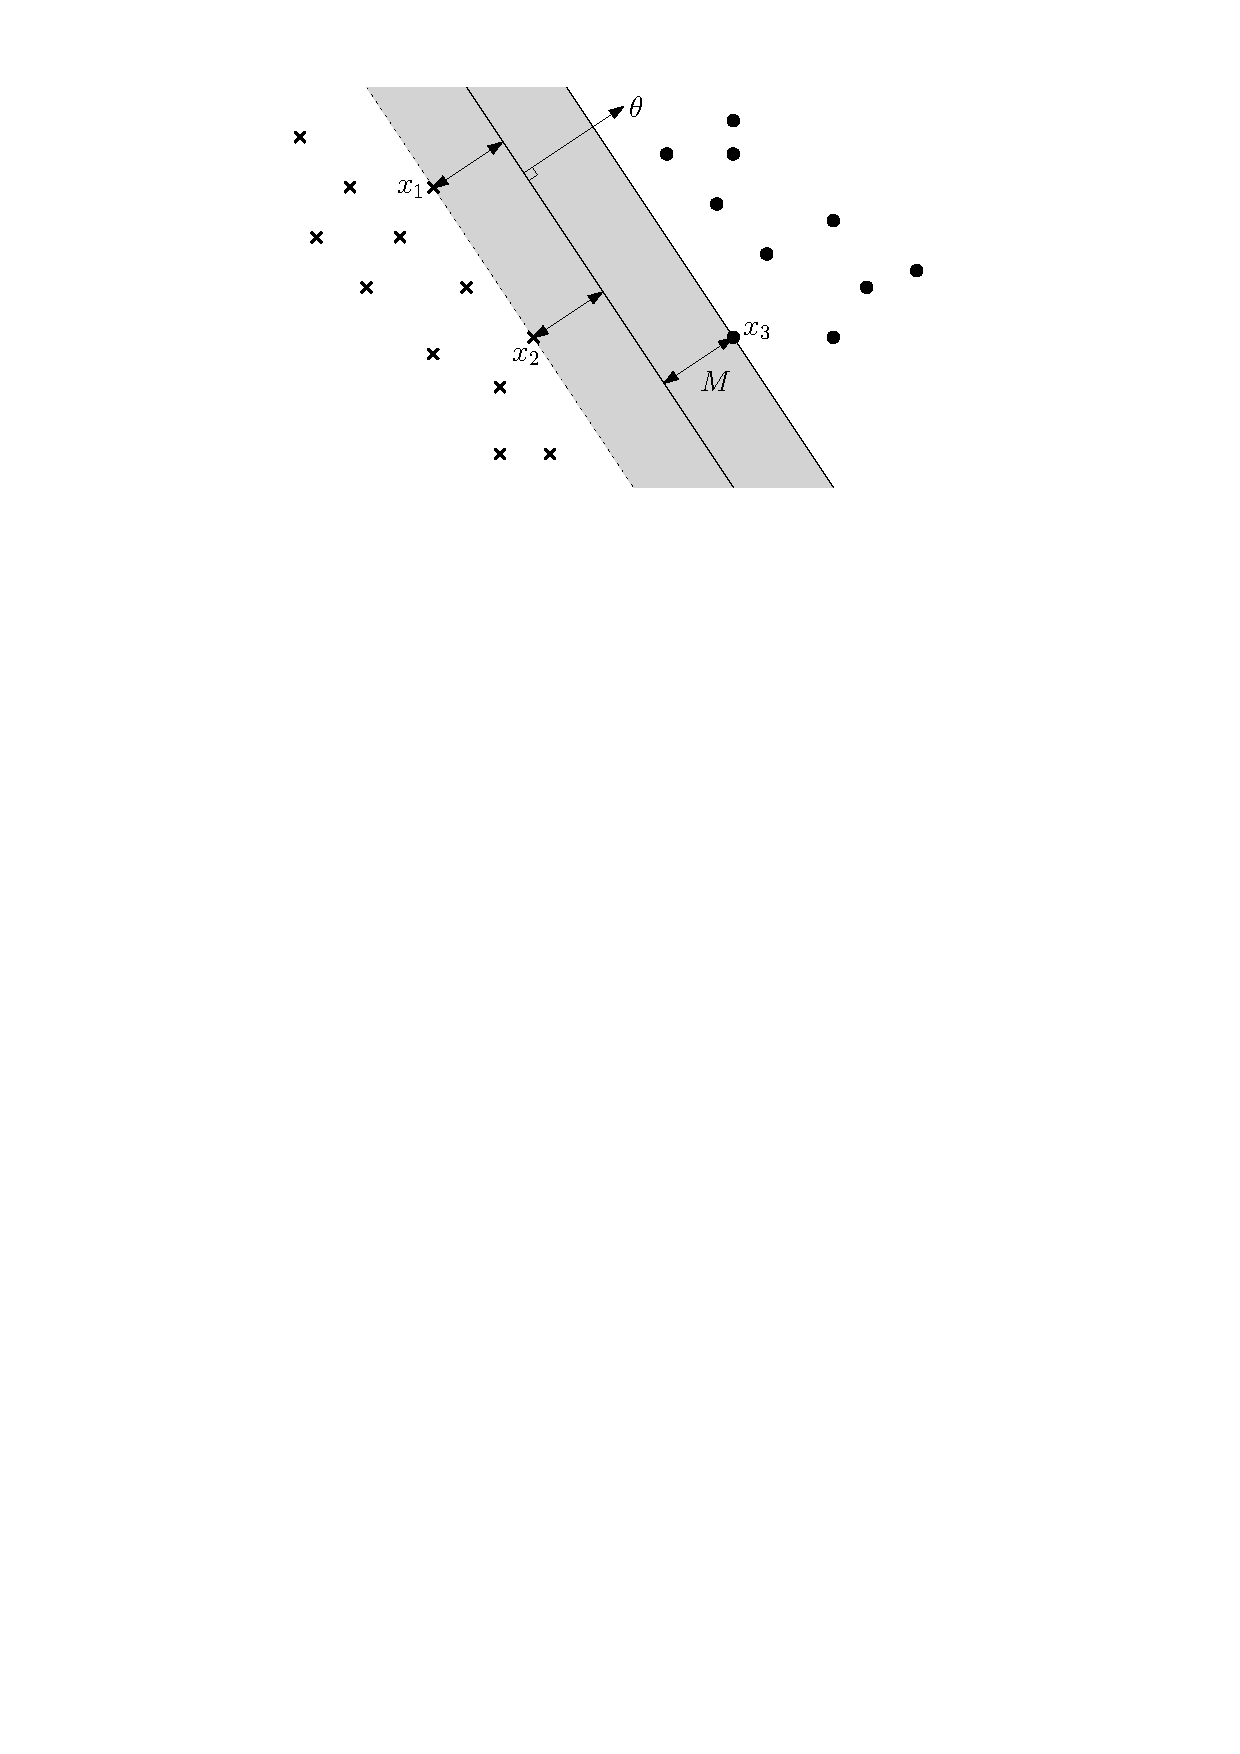
\includegraphics[width = 5cm]{figures/Margin} 
\caption{\label{fig:sephyp} Example of separating hyperplane with three support vectors.} 
\end{figure} 

Without any loss of generality, we restrict ourselves to hyperplanes for which points achieving the minimal distance 
lie on the two parallel hyperplanes $\langle x,\theta\rangle-b=1$ and 
$\langle x,\theta\rangle-b=-1$. This leads to $M\|\theta\|_2=1$ and thus $M=\|\theta\|_2^{-1}$. 
Maximizing $M$ is then minimizing $\|\theta\|_2$. Finally, to have a quadratic problem, we choose to 
minimize $\|\theta\|_2^{2}/2$ instead of $\|\theta\|_2$. %, because $\text{argmin }\|\theta\|=\text{argmin }\|\theta\|^{2}/2$. 
The problem becomes: 

$$\inf_{\theta,b}\ \frac{\|\theta\|_2^{2}}{2}\text{ subject to }y_{i}(\langle x_i,\theta\rangle-b)\ge 1,\text{ for all }1\leq i\leq n.$$ 

This is a quadratic convex optimization problem with linear constraints, hence the solution is unique. 
It can be solved by introducing a Lagrangian 
$L(\theta,b,\lambda) = \frac{\|\theta\|_2^{2}}{2}+\sum_{i=1}^{n}\lambda_{i}(1-y_{i}(\langle x_{i},\theta\rangle-b))$ 
(with $\lambda\in\mathbb{R}_+^n$) and using a strong duality between primal and dual solution, which means our solution 
is also the solution of the problem: 

$$\sup_{\lambda}\ \inf_{\theta,b}\ L(\theta,b,\lambda),$$

%or equivalently $\max_\lambda\ g(\lambda)$ (where $g(\lambda)=\text{min}_{\theta,b}\ L(\theta,b,\lambda)$)  and: 
%$\min_{\theta,b}\ \text{max}_{\lambda}\ L(\theta,b,\lambda)$ 

Let $g(\lambda)=\inf_{\theta,b}\ L(\theta,b,\lambda)$.
Let $\lambda^{*},\theta^{*},b^{*}$ be the solutions to this problem.

\begin{itemize}

\item If $\sum\lambda_{i}y_{i}\neq 0$, then $g(\lambda)=-\infty$ because of the scalar $b$. Hence $\sum\lambda^{*}_{i}y_{i}=0$.

\item The condition $\nabla_{\theta}L=0$ leads to $\theta^{*}=\sum\lambda^{*}_{i}y_{i}x_{i}$. 
Thus, if we replace $\theta^{*}$ by its expression, $\lambda^{*}$ becomes the 
unique solution of the problem: 
$$\max_\lambda\ \sum_{i}\lambda_{i}-\frac{1}{2}\sum_{i,j}\lambda_{i}\lambda_{j}y_{i}y_{j}\langle x_{i},x_{j}\rangle\text{ subject to }
\lambda_{i}\geq 0, \sum_{i}\lambda_{i}y_{i}=0,\text{ for all }1\leq i\leq n.$$ 
which can be found by quadratic programming. Thus, we can first compute $\lambda^{*}$ and then $\theta^{*}$.

\item Now, if $L(\theta^{*},b^{*},\lambda^{*})$ is equal to the solution of the original problem, 
then we necessarily have for all $i$: 
$$\lambda^{*}_{i}(1-y_{i}(\langle x_{i},\theta^{*}\rangle-b^{*}))=0.$$ 
Thus, either $\lambda^{*}_{i}=0$ or $\lambda^{*}_{i}\neq 0$ and $y_{i}(\langle x_{i},\theta^{*}\rangle-b^{*})=1$. 
Hence, first we can compute $b^{*}$ if $\lambda^{*}_{i}\neq 0$ 
for some $i$ with $b^{*}=\langle x_{i},\theta^{*}\rangle-y_{i}$, and second, if $\lambda^{*}_{i}\neq 0$, 
then $x_{i}$ is exactly at the minimal margin, it is called a {\em support vector}.
\end{itemize}

%We recall that we want to classify the $m$ variables $z_{k}\in\mathbb{R}^{D}$.
The final classifier is: $c(x)=\text{sign}\ \langle\theta^{*},x\rangle-b^{*}=\text{sign}\ \sum_{i}\lambda^{*}_{i}y_{i}\langle x_{i},x\rangle-b^{*}$, 
where $\theta^{*}$ and $b^{*}$ are set up at the learning step. This classifier takes the sign of the 
so-called {\em posterior}. It depends only on the support vectors since $\lambda_i^*=0$ for the other vectors.

%\section{Non Separable Data}

\subsection{C-SVM}\label{sec:CSVM}

\paragraph*{Slack variables.} If the $x_{i}$ are not separable, which is often the case in practice, we can change the problem a little bit by 
introducing {\em slack variables} $\xi_{i}$ that will measure the degree of non separability of 
the data. We have the following problem: 
$$\inf_{\theta,b}\ \frac{\|\theta\|_2^{2}}{2}+C\sum_{i}\xi_{i}\text{ such that }\xi_{i}\ge 0,\ \xi_{i}\ge 1-y_{i}(\langle x_{i},\theta\rangle-b)\text{ for all }1\leq i\leq n.$$ 
Thus, if $x_{i}$ has a margin greater than 1, then we can take $\xi_{i}=0$ because $1-y_{i}(\langle x_{i},\theta\rangle-b)$ is negative. 
But if $x_{i}$ has a margin less than 1, and possibly negative, then $1-y_{i}(\langle x_{i},\theta\rangle-b)$ is positive, so we want 
to minimize these above-margin points. This is called $C$-SVM. The choice of the cost $C$ can be done through several 
standard techniques, like cross validation for instance. Note that when $C\rightarrow\infty$, we go back to 
the previous problem. Finding the optimal $\theta$ and $b$ can be done essentially in the same way as before, as it is also 
a quadratic convex optimization problem. 

\paragraph*{Optimization.} We use strong duality with the Lagrangian: 

$$L(\theta,b,\xi,\lambda,\nu) = \frac{\|\theta\|_2^{2}}{2}+C\sum_{i=1}^{n}\xi_{i}-
\sum_{i=1}^{n}\lambda_{i}(y_{i}(\langle x_{i},\theta\rangle-b)-1+\xi_{i})-\sum_{i=1}^{n}\nu_{i}\xi_{i},$$

with $\lambda,\nu\in\mathbb{R}_{+}^{n}$.
Once again, $g(\lambda,\nu)=\text{min}_{\theta,b,\xi}\ L(\theta,b,\xi,\lambda,\nu)$ and 
we call $\lambda^{*},\nu^{*},\theta^{*},b^{*},\xi^{*}$ the solutions of this problem.

\begin{itemize}
\item[1.] If $\sum\lambda_{i}^{*}y_{i}\neq 0$, $g(\lambda^{*},\nu^{*})=-\infty$. Hence $\sum\lambda^{*}_{i}y_{i}=0$.
\item[2.] Setting $\nabla_{\theta}\ L=0$ gives $\theta^{*}=\sum_i\lambda^{*}_{i}y_{i}x_{i}$.
\item[3.] Setting $\nabla_{\xi}\ L=0$ gives $\lambda_{i}^{*}+\nu_{i}^{*}=C$, for all $i$.
\item[4.] If $L(\theta^{*},b^{*},\xi^{*},\lambda^{*},\nu^{*})$ is equal to the solution of the original problem, then we have necessarily for every $i$:
\begin{itemize}
\item[(i).] $\lambda^{*}_{i}(y_{i}(\langle x_{i},\theta^*\rangle-b^{*})-1+\xi^{*}_{i})=0$
\item[(ii).] $\nu^{*}_{i}\xi^{*}_{i}=0$ 
\item[(iii).] $\xi_{i}^{*}\ge 0$
\item[(iv).] $y_{i}(\langle x_{i},\theta^*\rangle-b^{*})-1+\xi^{*}_{i}\ge 0$
\end{itemize}
\end{itemize}

After replacing $\theta^{*}$ by its expression, $\lambda^{*}$ and $\nu^{*}$ becomes the solutions of 
the dual problem: 

$$\sup_{\lambda,\nu} \sum_{i}\lambda_{i}y_{i}-\frac{1}{2}\sum_{i,j}\lambda_{i}\lambda_{j}y_{i}y_{j}\langle x_{i},x_{j}\rangle\text{ subject to }
\lambda_{i}+\nu_{i}=C,\ \sum_{i}\lambda_{i}y_{i}=0,\lambda_{i}\ge 0,\nu_{i}\ge 0.$$ 

As $\nu$ only appears in the condition, we can get rid of it and we finally obtain: 
$$\sup_{\lambda} \sum_{i}\lambda_{i}y_{i}-\frac{1}{2}\sum_{i,j}\lambda_{i}\lambda_{j}y_{i}y_{j}\langle x_{i},x_{j}\rangle\text{ subject to }
0\leq\lambda_{i}\leq C,\ \sum_{i}\lambda_{i}y_{i}=0.$$

Once again, we can compute the $\lambda_{i}^{*}$ by quadratic programming. 
We can then compute $\theta^{*}=\sum\lambda^{*}_{i}y_{i}x_{i}$. If there is some $i$ such that $0<\lambda^{*}_{i}<C$, we 
can compute $b^{*}$ because we have from 3. that $0<\nu^{*}_{i}<C$, then, with 4.(ii), $\xi^{*}_{i}=0$ and finally, 
with 4.(i): $b^{*}=x_{i}^{T}\theta^{*}-y_{i}$. \\

The final classifier is again : $c(x)=\text{sign}\ \langle\theta^{*},x\rangle-b^{*}=\text{sign}\ \sum_{i}\lambda^{*}_{i}y_{i}\langle x_{i},x\rangle-b^{*}$.
There is an interesting interpretation: 

\begin{itemize}
\item If $y_{i}(\langle x_{i},\theta^{*}\rangle-b^{*})>1$, then it follows from 4.(i) that $\lambda^{*}_{i}=0$ because $\xi^{*}_{i}\ge 0$. Hence, 
well classified points with margin superior to the minimal margin have no impact.

\item If $y_{i}(\langle x_{i},\theta^{*}\rangle-b^{*})<1$, then it follows from 4.(iv) that $\xi_{i}^{*}>0$. Thus we have from 4.(ii) that 
$\nu_{i}^{*}=0$ and, from 3., $\lambda_{i}^{*}=C$. Hence, badly classified points with margin inferior to minus the minimal margin
have maximal weight.
\end{itemize}

\end{comment}


\section{Supervised Machine Learning}\label{sec:learning}

In this section, we briefly recall the basics of supervised Machine Learning and kernel methods.
We refer the interested reader to~\cite{Friedman01} and~\cite{Shawe04} for further details.

In the context of supervised Machine Learning, you are given $n$ observations 
$(x_1,y_1),\cdots,(x_n,y_n)\in X\times Y$, where $X$ is the space of data and $Y$ is the space of targets---generally, 
targets are discrete labels in classification, and continuous variables in regression for instance.
The goal is to produce a predictor $f_n:X\rightarrow Y$, which is built only from the observations: $f_n=f_n((x_1,y_1),\cdots,(x_n,y_n))$
and as accurate as possible. Accuracy is usually measured with {\em loss functions}, that we now detail.

  

\subsection{Empirical Risk Minimization}

Predictors in supervised Machine Learning are computed as the minima of the following general equation:

\begin{equation}\label{eq:ERM}
f^* = {\rm argmin}_{f\in\mathcal{F}}\ {\rm ER}_n(f) = {\rm argmin}_{f\in\mathcal{F}}\ \frac 1n \sum_{i=1}^n L(y_i,f(x_i)) + \Omega(f), 
\end{equation}

where $\mathcal F$ is a class of predictors, 
$L:Y\times Y\rightarrow \R$ is a {\em loss function} measuring the error made by $f$ on the training observations,
$\Omega(f)$ is a {\em regularization term} used to avoid overfitting and too complicated predictors,
and ${\rm ER}_n(f)$ is called the {\em empirical risk} of $f$.

\paragraph*{Loss functions.} Several different loss functions exist in the literature, each corresponding to 
a specific Machine Learning algorithm. Assuming $Y\subseteq\R$, examples of such losses include:

\begin{itemize}
\item $L(y_i,f(x_i))=\delta_{y_i=f(x_i)}$, known as the {\em zero-one loss}. Due to its non smoothness,
%solving Equation~\ref{eq:ERM} 
minimizing the empirical risk with this loss may become NP-hard, even for simple classes of predictors.
\item $L(y_i,f(x_i))=\max\{0, 1-y_if(x_i)\}$, known as the {\em hinge loss}. It is used in Support Vector Machine prediction.
Even though it is not smooth, %Equation~\ref{eq:ERM} 
the empirical risk can be minimized efficiently with it.
\item $L(y_i,f(x_i))={\rm log}(1+{\rm exp}(-y_if(x_i)))$, known as the {\em log loss}. It is used in Logistic regression.
\item $L(y_i,f(x_i))={\rm exp}(-y_if(x_i))$, known as the {\em exponential loss}. It is used in Adaboost prediction.
\item $L(y_i,f(x_i))=(y_i - f(x_i))^2$, known as the {\em squared loss}. It is used in least square regression.
\end{itemize}

\paragraph*{Regularization term.}  Regularization terms are often used when the class $\mathcal F$
 is parametrized by vectors of Euclidean space $\mathcal F=\{f_w\,:\,w\in\R^D\}$. In this
case, the most common regularizes are:

\begin{itemize}
\item $\Omega(f_w)=\langle w,w\rangle=\|w\|_2^2$, known as {\em $\ell_2$ regularization}. It is strictly convex and differentiable,
hence the empirical risk %Equation~\ref{eq:ERM} 
can be optimized efficiently. However, the solution $w^*$ may be {\em dense}, i.e. with many nonzero coordinates.
\item $\Omega(f_w)=\|w\|_1$, known as {\em $\ell_1$ regularization}. It is convex and not differentiable at $0$, but the
solution  $w^*$ is in general {\em sparse}, i.e. with just a few nonzero coordinates.
\item $\Omega(f_w)=\alpha\|w\|_1 + (1-\alpha)\|w\|_2^2$, where $0\leq \alpha < 1$, known as {\em elastic net regularization}.
\item $\Omega(f_w)=\|w\|_p$, where $0<p\leq 1$, known as {\em $\ell_p$ regularization}.
\end{itemize}

The difficulty of minimizing the empirical risk
%Equation~\ref{eq:ERM} 
also depends a lot on the class of predictors $\mathcal F$. 
It is greatly simplified when $\mathcal F$ is a {\em reproducing kernel Hilbert space} (RKHS). 
%We will detail such spaces in the next section. 
%Before, we conclude this section with few very common special cases of losses and
%regularizer used in Machine Learning.

%\begin{itemize}
%\item {\em Support Vector Machine} minimizes the following empirical risk:
%\end{itemize}  

\subsection{Reproducing Kernel Hilbert Space}

RKHSs are Hilbert spaces of functions for which function evaluation at a specific point $x$ can be computed with scalar products.

\begin{defin}
A set $\mathcal H\subset \R^X$ forming a Hilbert space, with scalar product $\langle\cdot,\cdot\rangle_{\mathcal H}$, is
a {\em reproducing kernel Hilbert space} if there exists a function $k:X\times X\rightarrow\R$, called a {\em kernel}, such that:
\begin{itemize}
\item[\rm (i)] $\{k_x\,:\,x\in X\}\subset\mathcal H$, where $k_x:x\mapsto k(x,\cdot)$, and
\item[\rm (ii)] $f(x)=\langle f,k_x \rangle_{\mathcal H}$, for any $x\in X$ and $f\in\mathcal H$.
\end{itemize}
\end{defin} 

An equivalent definition is to require that the evaluation function 
$F_x:\mathcal H\rightarrow\R$ defined by $F_x(f)=f(x)$ 
is continuous for any $x\in X$.

%For instance, Euclidean space $\R^D$ is a RKHS, with kernel $k(x,y)=\langle x,y \rangle$.

\begin{prop}
The kernel of a RKHS is unique and, conversely, a function $k$ can be the kernel of at most one RKHS.
Hence, one can talk of {\em the} kernel of a RKHS. 
\end{prop}



There is a useful characterization of kernels
with {\em positive semi-definite} functions.

\begin{thm}[Moore-Aronszajn~\cite{Aronszajn50}] 
A function $k:X\times X\rightarrow\R$ is a kernel if and only if it is positive semi-definite,
i.e. $\sum_{i,j}a_ia_jk(x_i,x_j)\geq 0$ for any $a_1,\cdots,a_n\in\R$ and $x_1,\cdots,x_n\in X$.
\end{thm}

When $X=\R^D$, $D\in\N^*$, examples of such positive semi-definite functions include:
\begin{itemize}
\item the linear kernel: $k(x,y) = \langle x, y \rangle$,
\item the polynomial kernel: $k(x,y) = (\alpha \langle x, y \rangle + 1)^\beta$, $\alpha,\beta\in\R$,
\item the Gaussian kernel: $k(x,y) = \exp\left( -\frac{\|x-y\|_2^2}{2\sigma^2}\right)$, $\sigma >0$.
\end{itemize}


Minimizing the empirical risk when $\mathcal F$ is a RKHS $\mathcal H$ turns out to be easy, even when $\mathcal H$ is infinite dimensional,
as is the case for many kernels.

\begin{thm}[Representer Theorem~\cite{Scholkopf01}]
Let $(x_1,y_1),\cdots,(x_n,y_n)\in X\times Y$ be $n$ observations, and
let $k:X\times X\rightarrow\R$ be a kernel, i.e. a positive semi-definite function,
with corresponding RKHS $\mathcal H$.
Let $\Omega:\R_+\rightarrow\R$ be a strictly monotonically increasing function,
and $L:Y\times Y\rightarrow\R$ be an arbitrary loss function.
Then, any function $f^*\in\mathcal H$ minimizing
$$\frac 1n \sum_{i=1}^n L(y_i,f(x_i)) + \Omega(\|f\|_{\mathcal H})$$
is of the form $f^*(\cdot)=\sum_{i=1}^n \alpha_i k(x_i,\cdot)$, where $\alpha_1,\cdots,\alpha_n\in\R$.
\end{thm} 

In particular, computing $f^*$ does not require to know the RKHS $\mathcal H$; only the 
evaluations of the kernel at the observations $k(x_i,x_j)$ are necessary. 


\paragraph*{The kernel trick.} %\label{sec:kerneltrick}
%An alternative view of RKHS 
A direct consequence of the previous results is the following theorem:  %, which comes from the following theorem:

\begin{cor}
For any kernel $k:X\times X\rightarrow\R$, 
there exists a essentially unique Hilbert space $\mathcal H$ and an embedding $\Phi:X\rightarrow\mathcal H$ such that: 
$$k(x,y)=\langle\Phi(x),\Phi(y)\rangle_{\mathcal H}.$$
\end{cor}


Hence, any set $X$ can be seen as a subset of a Hilbert space, as soon as there is a positive semi-definite function, or kernel, at hand.
This is attractive since observations in this Hilbert space may be linearly separable, even if the observations themselves are not.
This is known as the {\em kernel trick}.
See Figure~\ref{fig:trick}. 

\begin{figure}[h]\centering  
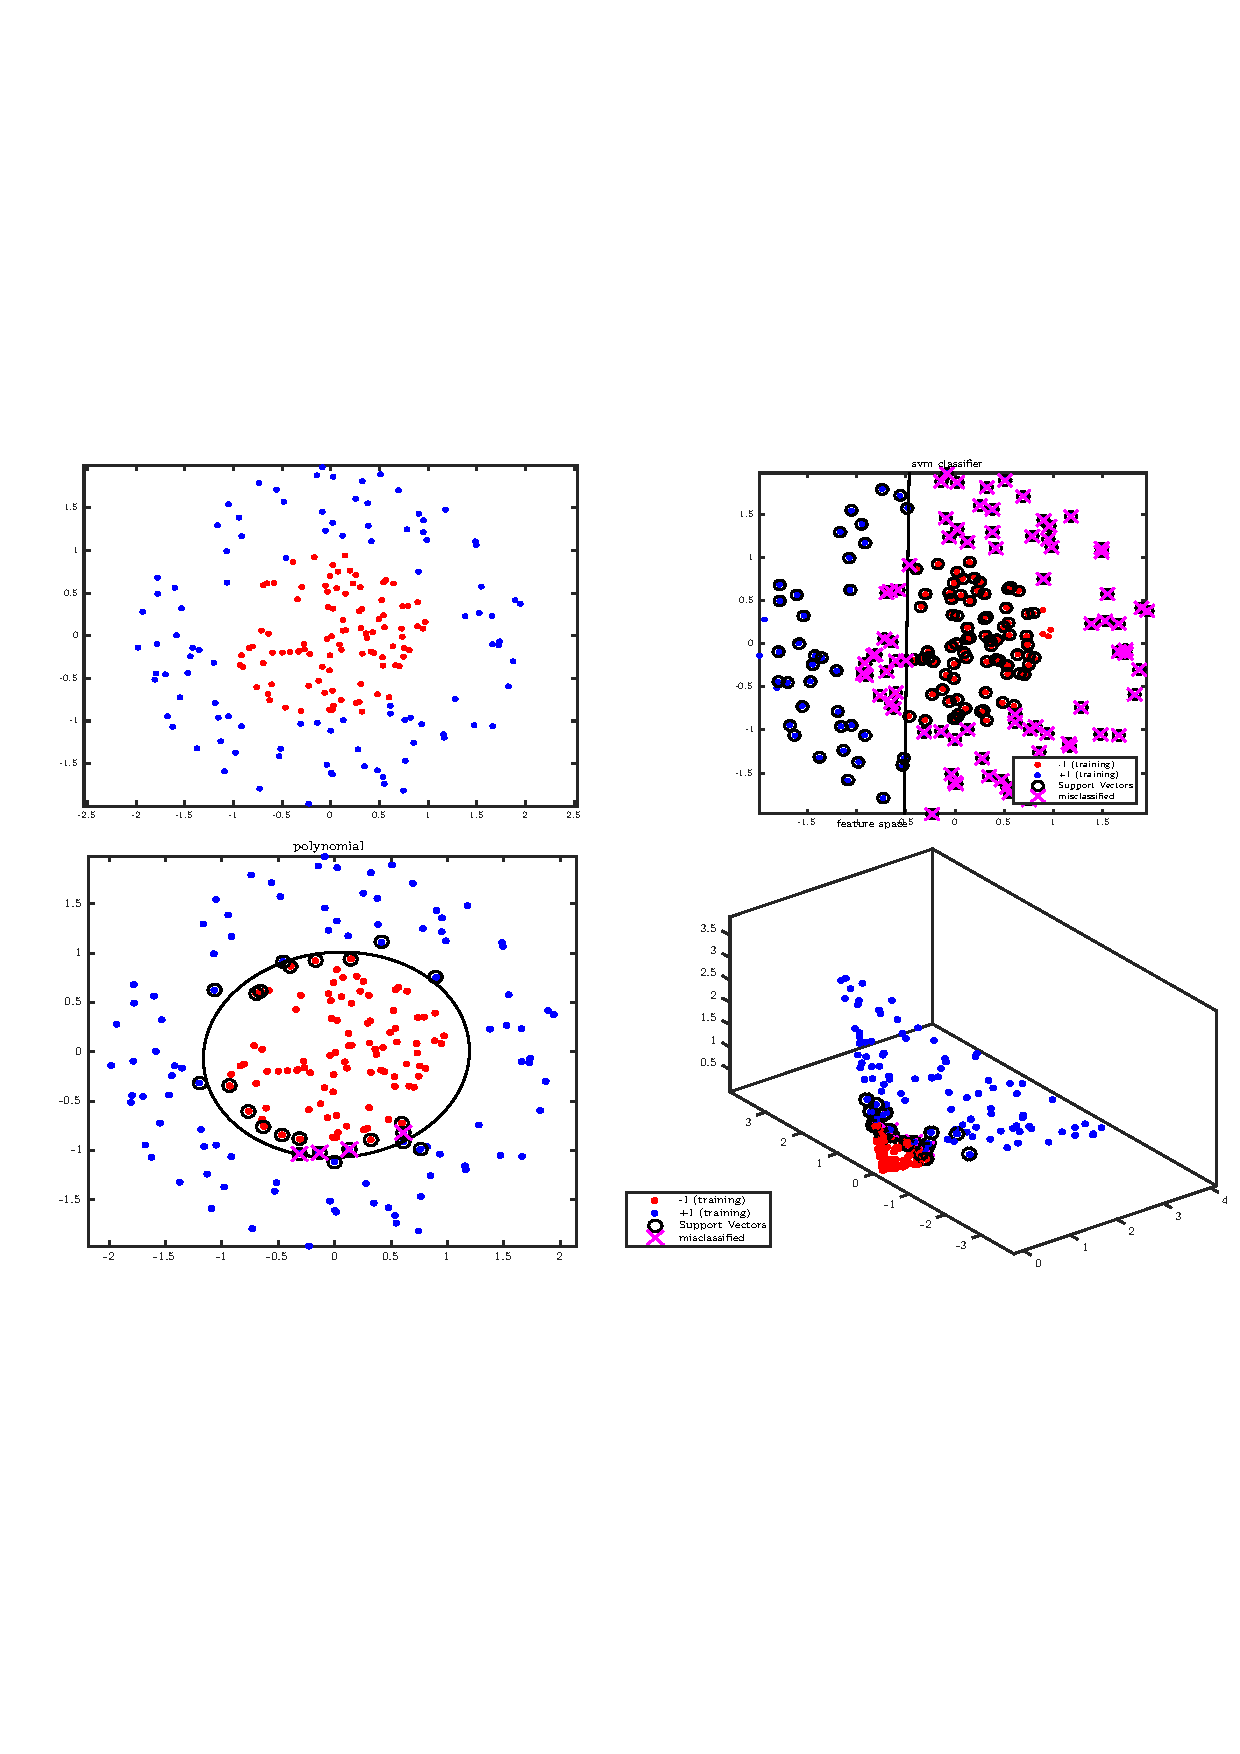
\includegraphics[width = 15cm]{figures/KernelTrick} \caption[Kernel trick]{\label{fig:trick} 
In $\mathbb{R}^{2}$, red points
cannot be separated from blue ones with a line without producing misclassified points (first row). However, embedding these points 
into $\mathbb{R}^{3}$, for instance with a polynomial kernel, can make them separable. It then suffices to push back the separating hyperplane in $\R^3$
to get a non linear separation in $\R^2$ (second row).   
%would give a positive height to disks and a null height to crosses makes the data separable, as we can now find a separating plane. 
} 
\end{figure} 

%The main idea behind the kernel trick is that, if the data is non separable, maybe it is 
%when we send it into a much bigger space---see the example in Figure~\ref{fig:trick}. 
%Suppose that we have now such a good map $\Phi:\mathcal X\rightarrow\mathcal H$, where $\mathcal H$ 
%is a Hilbert space and $\mathcal X$ is the data set (not necessarily $\R^D$). We will apply a $C$-SVM to the data $(\Phi(x_{1}),\cdots,\Phi(x_{n}))$.
%The problem now becomes: 
%$$\min_{\theta,b}\ \|\theta\|_2^{2}/2+C\sum_{i}\xi_{i}\text{ subject to }\xi_{i}\ge 0,\ \xi_{i}\ge 1-y_{i}(\langle\Phi(x_{i}),
%\theta\rangle-b)\text{ for all }1\leq i \leq n,$$ 
%and the final classifier is of the form: 
%$$c(x)=\text{sign}\ \langle\theta^{*},\Phi(x)\rangle-b^{*}=\text{sign}\ \sum_{i}\lambda^{*}_{i}y_{i}\langle\Phi(x_{i}),\Phi(x)\rangle-b^{*}.$$

%However, it can be very difficult in practice to find such a $\Phi$. 
%Since the solution and the final classifier only depend on the $\langle\Phi(x_{i}),\Phi(x_{j})\rangle$,
%the question becomes, given a similarity function (or {\em kernel}) $k$ between points, whether it is possible to find
%a Hilbert space and a map $\Phi$ such that $k(x_i,x_j)=\langle\Phi(x_i),\Phi(x_j)\rangle_{\mathcal H}$.  
%The following Theorem answers this question:

%\begin{thm}[Moore-Aronszajn~\cite{Aronszajn50}] 
%If $k$ is a symmetric positive semi-definite kernel on 
%$\mathcal X\times\mathcal X$, then there exists a Hilbert space $\mathcal H$ and 
%a feature map $\Phi:\mathcal X\rightarrow\mathcal H$ such that 
%$\forall x,x'\in\mathcal X$, $$k(x,x')=\langle \Phi (x),\Phi(x')\rangle_{\mathcal H}.$$
%\end{thm}

%Then, the classifier becomes: 
%$$c(x)=\text{sign}\ \sum_{i}\lambda^{*}_{i}y_{i}k(x_i,x)-b^{*}$$ 
%where the $\lambda^{*}_{i}$ are solutions of: 
%$$\sup_{\lambda} \sum_{i}\lambda_{i}y_{i}-\frac{1}{2}\sum_{i,j}\lambda_{i}\lambda_{j}y_{i}y_{j}k(x_{i},x_{j})\text{ subject to }
%0\leq\lambda_{i}\leq C,\ \sum_{i}\lambda_{i}y_{i}=0,\text{ for all }1\leq i \leq n.$$

%\paragraph*{Multi-Labeling.}
%We recall that in our problem, there can be more than 2 labels. 
%For instance, a human can be separated in head, legs, arms, torso... If we need 
%to treat more than 2 labels, 
%In the case of multiple labels, the most common technique is one-versus-all classifiers: 
%for each label $y$, we train a kernel $C$-SVM on the training points, where a point has 
%label $1$ if the ground truth label of this point is $y$ and $-1$ otherwise. Hence, we get 
%separating hyperplanes $(\theta_y,b_y)$ for each label $y$. 
%a vector $P_{y}$ of size the number of test points. 
%This vector has at row $k$, the posterior of $z_{k}$, normalized 
%by the maximal posterior. 
%Finally, we take as label for $x$ the label giving the maximal posterior: 
%$\text{argmax}_{y}\ \langle\theta^*_y,x\rangle-b^*_y$.

\paragraph*{Gaussian kernels.} A standard way to derive a kernel is to exponentiate the negative of a 
squared Euclidean distance. This is due to the following result of Berg et al:

\begin{thm}[Theorem 3.2.2 of~\cite{Berg84}]\label{th:berg}
%The Gaussian kernel for vectors with parameter $\sigma>0$ does follow that template approach: 
%$k_\sigma(x,y)={\rm exp}\left(-\frac{\|x-y\|^2}{2\sigma^2}\right)$. An important theorem of (, p.74) states that 
%such an approach to build kernels, namely 
Let $\sigma >0$. The Gaussian function $$k_\sigma(x,y)= {\rm exp}\left(-\frac{f(x,y)}{2\sigma^2}\right),$$
for an arbitrary function $f$, is positive semi-definite for all $\sigma>0$ 
if and only if $f$ is a \emph{conditionally negative semi-definite} function, i.e. $\sum_{i,j}a_ia_jf(x_i,x_j)\leq 0$
for any $n \in\N^*$, $x_1,\cdots,x_n \in X$, and $ a_1,\cdots,a_n \in \R$ such that $\sum_ia_i=0$.
\end{thm}

%\paragraph*{Kernels for Persistence Diagrams.}
Concerning persistence diagrams, it has been observed in Appendix~A of~\cite{Reininghaus14} that, 
unfortunately, the metrics $\distb$ or $\distw{1}$ %---see Definition~\ref{def:bottleneck}, 
are not conditionally negative semi-definite 
(it suffices to randomly sample a family of point 
clouds to observe experimentally that more often than not the inequality of negative definiteness will be violated for particular weights $a_1,\cdots,a_n$). 
In the following section, we present an approximation of $\distw{1}$ with the {\em Sliced Wasserstein distance}, which is provably 
conditionally negative semi-definite, and we use it to define a Gaussian kernel that can be easily tuned thanks to its bandwidth parameter $\sigma$.
























\section{A Gaussian Kernel for Persistence Diagrams}
\label{sec:GaussianPDs}

Several infinite dimensional kernels have been derived for persistence diagrams within the last few years.
For instance, in~\cite{Reininghaus15}, the authors use
solutions of the heat differential equation in the plane, with initial heat sources located at the persistence diagram points, and compare them
with the usual $L^2(\R^2)$ scalar product.
Differently, in~\cite{Kusano16}, the authors treat a persistence diagram as a discrete measure on the plane,
and follow by using kernel mean embeddings with Gaussian kernels---see Section~\ref{sec:expe} for precise definitions.
Both kernels are provably {\em stable}, in the sense that the metric they induce in their respective RKHS 
is bounded above by the distance between persistence diagrams. 
Although these kernels are injective, there is no evidence that their induced RKHS distances are {\em discriminative}, and thus follow 
the geometry of the bottleneck or Wasserstein distances for persistence diagrams.
In this section, we present the {\em Sliced Wasserstein} kernel for persistence diagrams, which is 
both stable and discriminative if the diagrams have bounded cardinalities. The kernel is based on a modification of
the Wasserstein distance between probability measures, that we first define. 
%present in Section~\ref{sec:wasserstein}. The
%kernel is then defined in Section~\ref{sec:SWK}, and its metric properties are studied in Section~\ref{sec:metricKernel}.
%Finally, algorithms for computation are provided in Section~\ref{sec:comput}, and experiments are done is Section~\ref{sec:expe}.


\subsection{Wasserstein distance for unnormalized measures on $\mathbb{R}$}
\label{sec:wasserstein}

%In this Section, we review the {\em 1-Wasserstein distance} for {\em probability measures}.
%We use this distance in Section~\ref{sec:SWK} to define the Sliced Wasserstein distance for persistence diagrams
%seen as nonnormalized probability measures.

We first recall the basics on measures and integration. We refer the interested reader to~\cite{Bauer01} for further details.

\begin{defin}
Let $X$ be a set. A {\em $\sigma$-algebra} on $X$ is a collection $\mathcal E$ of subsets of $X$ such
that, for any $E\in\mathcal E$ and countable family $\{E_n\}_{n\in\N}$ in $\mathcal E$:

%\begin{itemize}
\begin{tabular}{lll}\vspace{-0.5cm} 
{\rm (i)} $\emptyset\in\mathcal E$, & {\rm (ii)} $(X\setminus E)\in\mathcal E$, &
{\rm (iii)} $\bigcup_{n\in\N}E_n\in\mathcal E$.  
\end{tabular}\vspace{0.5cm} 
%\end{itemize}

The pair $(X,\mathcal E)$ is called a {\em measurable space}.
\end{defin}

Given an arbitrary family $\mathcal S$ of subsets of $X$, the {\em $\sigma$-algebra generated by $\mathcal S$} is the smallest
$\sigma$-algebra containing every element of $\mathcal S$. If $X$ is a topological space, the $\sigma$-algebra generated by
the open sets of $X$ is called the {\em Borel algebra}.

\begin{defin}
A {\em measure} on a measurable space $(X,\mathcal E)$ is a function $\mu:\mathcal E\rightarrow\R\cup\{+\infty\}$ such that,
for any $E\in\mathcal E$ and countable family of {\em pairwise disjoint sets} $\{E_n\}_{n\in\N}$ in $\mathcal E$:

\begin{tabular}{lll}\vspace{-0.5cm} 
{\rm (i)} $\mu(E)\geq 0$, &
{\rm (ii)} $\mu(\emptyset)=0$, &
{\rm (iii)} $\mu\left(\bigcup_{n\in\N}E_n\right)=\sum_{n\in\N}\mu(E_n).$
\end{tabular}\vspace{0.5cm} 

A {\em probability} measure, sometimes called {\em normalized} measure, 
is a measure that also satisfies $\mu(E)\in[0,1]$ for any $E\in\mathcal E$ and $\mu(X)=1$.
\end{defin}

\begin{defin}
Let $(X,\mathcal E)$ be a measurable space.
Let $f:X\rightarrow\R_+$ be a measurable function, i.e. $f^{-1}([t,+\infty))\in\mathcal E$ for any $t\in\R$.
Let $\mu$ be a measure on $(X,\mathcal E)$. 

We define the integral of $f$ in several steps:
\begin{itemize}
\item If $f={\bf 1}_E$ where $E\in\mathcal E$, then $\int_X f{\rm d}\mu = \mu(E)$.
The function $f$ is called an {\em indicator function}.
\item If $f=\sum_i a_i {\bf 1}_{E_i}$, where $a_i>0$ and $E_i\in\mathcal{E}$, then 
$\int_X f{\rm d}\mu = \sum_i a_i\int_X{\bf 1}_{E_i}{\rm d}\mu = \sum_ia_i\mu(E_i).$
%with the convention that $0\times +\infty=0$.
The function $f$ is called {\em simple}.
\item %If $f\geq 0$, 
In general, we define the integral of $f$ as $\int_X f{\rm d}\mu = \sup\{\int_X s{\rm d}\mu\,:\, s\text{ is simple and }s\leq f\}$.
%\item In general, we decompose $f$ as the sum of two nonnegative functions: $f=f^+-f^-$, where $f^+(x)=f(x)$ if
%$f(x)>0$ and $0$ otherwise, and where $f^-(x)=-f(x)$ if $f(x)<0$ and $0$ otherwise.
%If either $\int_Xf^+{\rm d}\mu$ or $\int_Xf^-{\rm d}\mu$ is finite, we let $\int_Xf{\rm d}\mu=\int_Xf^+{\rm d}\mu - \int_Xf^-{\rm d}\mu$.
\end{itemize}
\end{defin}

The 1-Wasserstein distance $\mathcal W$~\cite[\S6]{Villani09} is a distance between probability measures. 
For reasons that will become clear in the next section, we focus here on a variant of that distance: 
the 1-Wasserstein distance for nonnecessarily normalized measures on the real line~\cite[\S2]{Santambrogio15}. 

\begin{defin}
Let $\mu$ and $\nu$ be two measures on the real line such that 
$\mu(\mathbb{R})=\nu(\mathbb{R})=r>0$. 
The 1-Wasserstein distance between $\mu$ and $\nu$ is:
\begin{equation}\label{eq:optimal}
\distwm(\mu,\nu)=\inf_{\xi\in\Pi(\mu,\nu)} \iint_{\mathbb{R}\times\mathbb{R}} |x-y| {\rm d}\xi(x,y),
\end{equation}
where $\R^2$ is equipped with the Borel algebra and  
$\xi\in\Pi(\mu,\nu)$ is a measure on $\mathbb{R}^2$ with marginals $\mu$ and $\nu$, i.e. $\xi(\cdot,\R)=\mu$ and $\xi(\R,\cdot)=\nu$.
\end{defin}

This distance enjoys two good properties: it is {\em conditionally negative semi-definite} and {\em additive}.
To show this, let us define the two following distances:

\begin{align}
%&\distwm(\mu,\nu)=\inf_{\xi\in\Pi(\mu,\nu)} \iint_{\mathbb{R}\times\mathbb{R}} |x-y| {\rm d}\xi(x,y)\label{eq:optimal}\\
&\mathcal{Q}_r(\mu,\nu)=r \int_{[0,1]} | M^{-1}(x)- N^{-1}(x)| {\rm d}x\label{eq:quantile}\\
&\mathcal{L}(\mu,\nu)=\inf_{f\in 1\text{-Lipschitz}}\int_{\mathbb{R}} f(x) [\mu({\rm d}x)-\nu({\rm d}x)],\label{eq:Kanto}
\end{align}

where $M^{-1}$ and $N^{-1}$ are the quantile functions of the probability measures $\frac 1r \mu$ and $\frac 1r \nu$ respectively, i.e.
$M(x)=\frac 1r \mu((-\infty,x])$ and $N(x)=\frac 1r \nu((-\infty,x])$. 

\begin{prop}\label{prop:wasser1D}
We have $\mathcal{W}=\mathcal{Q}_r=\mathcal{L}$. 
Additionally:

\begin{tabular}{l}
\emph{(i)} $\mathcal{Q}_r$ is conditionally negative semi-definite on the space of measures of mass $r$; \\
\emph{(ii)} for any positive measures $\mu,\nu,\gamma$ such that $\mu(\R)=\nu(\R)$, 
we have $\mathcal{L}(\mu+\gamma,\nu+\gamma)=\mathcal{L}(\mu,\nu)$.
\end{tabular}
\end{prop}

\begin{proof} %Equation~(\ref{eq:optimal}) is the generic Kantorovich formulation of optimal transport, which is easily generalized to 
%other cost functions and spaces, the variant being that we consider an unnormalized mass by reflecting it directly 
%in the set $\Pi$. 
The equality between~(\ref{eq:optimal}) and~(\ref{eq:quantile}) is known for probability measures on the 
real line---see Proposition 2.17 in~\cite{Santambrogio15} for instance, and can be trivially generalized to unnormalized measures. 
%Because the cost function $|\cdot|$ is homogeneous, we see that the scaling factor $r$ can be removed when considering the quantile 
%function and multiplied back. 
The equality between~(\ref{eq:optimal}) and~(\ref{eq:Kanto}) is due to the well known Kantorovich duality for a distance 
cost~\cite[Particular case 5.4]{Villani09} which can also be trivially generalized to unnormalized measures, 
which proves the main statement of the proposition. 

The definition of $Q_r$ shows that the Wasserstein distance 
is the $l_1$ norm of $r M^{-1}- r N^{-1}$, and is therefore conditionally negative semi-definite (as the $l_1$ distance 
between two direct representations of $\mu$ and $\nu$ as functions $r M^{-1}$ and $r N^{-1}$), proving point (i). 
The second statement is immediate.
\end{proof}

We conclude this section with an important practical remark that concerns {\em empirical} measures. 

\begin{defin}
Let $(X,\mathcal E)$ be a measurable space.
A measure $\mu$ is said to be {\em empirical} if there exists a finite set of points $P\subset X$ such
that $\mu(E)=\card(E\cap P)$ for any $E\in\mathcal E$. In that case, we write $\mu=\sum_{p\in P}\delta_p$.
%to denote such a measure. 
Each $\delta_p$ is called a {\em Dirac measure} on $p$.
\end{defin}

\begin{rmq}\label{rq:empirical}
For two unnormalized empirical measures on the real line 
$\mu=\sum_{i=1}^n \delta_{x_i}$ and $\nu=\sum_{i=1}^n \delta_{y_i}$ of same total mass, with ordered 
$x_1\leq \cdots \leq x_{n}$ and $y_1\leq \cdots \leq y_{n}$, one has:
$$\distwm(\mu,\nu)=\sum_{i=1}^n|x_i-y_i|=\|X-Y\|_1,$$ 
where $X=(x_1,\cdots,x_n)\in\R^n$ and $Y=(y_1,\cdots,y_n)\in\R^n$.
\end{rmq}

\subsection{The Sliced Wasserstein Kernel}\label{sec:SWK}

\paragraph*{Sliced Wasserstein distance.} 
Any persistence diagram $\dg$ can be seen as an empirical measure on the plane $\mu=\sum_{p\in\dg}\delta_p$.
Hence, $\distwm$ can be computed on persistence diagrams. Since $\distwm$ is conditionally negative semi-definite 
when the measures are defined on the real line (Proposition~\ref{prop:wasser1D} and Remark~\ref{rq:empirical}), 
the idea of the Sliced Wasserstein distance of~\cite{Rabin11} is
to slice the plane with lines passing through the origin, to
project the measures onto these lines where $\mathcal W$ is computed, 
and to integrate the distances between the projected measures over all possible lines. 
 
%We now define a new kernel between persistence diagrams, called the {\em Sliced Wasserstein} (SW) kernel, 
%based on the Sliced Wasserstein metric . The idea underlying this
%metric is, when the persistence diagrams are seen as empirical measures,  Formally:

\begin{defin}  
Given $\theta\in\R^2$ with $\|\theta\|_2=1$, let $L(\theta)$ denote the line $\{\lambda\theta : \lambda\in\R\}$, and
let $\pi_\theta:\R^2\rightarrow L(\theta)$ be the orthogonal projection onto $L(\theta)$.
Let $\dg_1,\dg_2$ be two persistence diagrams, and let $\mu_1^\theta=\sum_{p\in \dg_1}\delta_{\pi_\theta(p)}$ and 
$\mu_{1\Delta}^\theta=\sum_{p\in \dg_1}\delta_{\pi_\theta\circ\pi_\Delta(p)}$,
and similarly for $\mu_2^\theta$, where $\pi_\Delta$ is the orthogonal projection onto the diagonal $\Diag$.
Then, the {\em Sliced Wasserstein distance} 
is defined as:
$$\SW(\dg_1,\dg_2)=\frac{1}{2\pi}\int_{\mathbb{S}_1} \mathcal W(\mu_1^\theta+\mu_{2\Delta}^\theta,\mu_2^\theta+\mu_{1\Delta}^\theta){\rm d}\theta.$$
\end{defin} 

We added the projections $\mu_{1\Delta}^\theta$ and $\mu_{2\Delta}^\theta$ because $\dg_1$ and $\dg_2$ may have different number of points,
Moreover, $\Delta$ counts for nothing in $\distb$ and $\distw{1}$.

Note that, by symmetry, one can restrict on the half-circle $[-\frac\pi2,\frac\pi2]$ and normalize by $\pi$ instead of $2\pi$.
Since $\mathcal W$ is conditionally negative semi-definite,
we can deduce that this is also true for $\SW$ itself. %is conditionally negative semi-definite:

\begin{lem}\label{lem:nd}
%Let $\SpfbD$ be the set of bounded and finite persistence diagrams. Then, 
$\SW$ is conditionally negative semi-definite on $\SpfbD$.
\end{lem}

%\begin{lem}\label{prop:p.d.}
%Let $X$ be a set of bounded and finite PDs.
%Then, $\SW$ is negative semi-definite on $X$.
%\end{lem} 



\begin{proof}

Let $n\in\mathbb{N}^*$, $a_1,...,a_n\in\R$ such that $\sum_ia_i=0$ and $\dg_1,...,\dg_n\in \SpfbD$.
Given $1\leq i\leq n$, we let 
$\tilde\mu_i^\theta=\mu_i^\theta + \sum_{q\in \dg_k,k\neq i}\delta_{\pi_\theta\circ\pi_\Delta(q)}$, 
$\tilde\mu_{ij\Delta}^\theta=\sum_{p\in \dg_k,k\neq i,j}\delta_{\pi_\theta\circ\pi_\Delta(p)}$ and
$d=\sum_i \card(\dg_i)$.
Then:
\begin{align}
&\sum_{i,j} a_ia_j \mathcal W(\mu_i^\theta+\mu_{j\Delta}^\theta,\mu_j^\theta+\mu_{i\Delta}^\theta)
=\sum_{i,j} a_ia_j\mathcal L(\mu_i^\theta+\mu_{j\Delta}^\theta,\mu_j^\theta+\mu_{i\Delta}^\theta)\nonumber \\
&=\sum_{i,j} a_ia_j\mathcal L(\mu_i^\theta+\mu_{j\Delta}^\theta+\mu_{ij\Delta}^\theta,\mu_j^\theta+\mu_{i\Delta}^\theta+\mu_{ij\Delta}^\theta)\nonumber\\
&= \sum_{i,j} a_ia_j\mathcal L(\tilde\mu_i^\theta,\tilde\mu_j^\theta)
= \sum_{i,j} a_ia_j\mathcal Q_d(\tilde\mu_i^\theta,\tilde\mu_j^\theta)\leq 0\nonumber
\end{align}  
The result follows by linearity of integration.


\end{proof}

Hence, Theorem~\ref{th:berg}
allows us to define a valid kernel on $\SpfbD$ with: 
%
\begin{equation}\label{eq:kSW}
\kSW(\dg_1,\dg_2)={\rm exp}\left(-\frac{\SW(\dg_1,\dg_2)}{2\sigma^2}\right).
\end{equation}



\subsection{Metric Preservation}\label{sec:metricKernel}


We now give the main theoretical result concerning the Sliced Wasserstein distance, 
which states that $\kSW$, in addition to be stable
and injective, preserves the metric between persistence diagrams, which should
intuitively lead to an improvement of the classification power. 
%$\SW$ is {\em equivalent} to $\distw{1}$.  
This has to be compared with~\cite{Reininghaus15} and~\cite{Kusano16}, which
only prove stability and injectivity. 
%Our equivalence result states that 
This intuition is illustrated in Section~\ref{sec:expe} and
Figure~\ref{fig:Airplanedistances}, where we show an improvement of
classification accuracies on several benchmark applications.

\paragraph*{Stability.} 
We first give an upper bound on the Sliced Wasserstein distance.

\begin{thm}\label{th:stab}
%Let $X$ be the set of bounded and finite PDs.
%Then, 
$\SW$  is stable with respect to $\distw{1}$ on $\SpfbD$, i.e.
for any $\dg_1,\dg_2\in \SpfbD$, one has: $$\SW(\dg_1,\dg_2)\leq 2\sqrt{2}\distw{1}(\dg_1,\dg_2).$$
\end{thm}

\begin{proof}
Let $\theta\in\R^2$ be such that $\|\theta\|_2=1$. Let $\dg_1,\dg_2\in \SpfbD$, and
let $\dg_1^\theta = \{\pi_\theta(p):p\in \dg_1\}\cup\{\pi_\theta\circ\pi_\Delta(q):q\in \dg_2\}$ and 
$\dg_2^\theta=\{\pi_\theta(q):q\in \dg_2\}\cup\{\pi_\theta\circ\pi_\Delta(p):p\in \dg_1\}$. % and $\mu_i,\mu_j$ be the corresponding signed empirical measures.
Let $\gamma^*$ be the one-to-one bijection between $\dg_1^\theta$ and $\dg_2^\theta$
induced by $\mathcal W(\mu_1^\theta+\mu_{2\Delta}^\theta,\mu_2^\theta+\mu_{1\Delta}^\theta)$, and
let $\gamma$ be the 
one-to-one bijection between $\dg_1\cup\pi_\Delta(\dg_2)$ and $\dg_2\cup\pi_\Delta(\dg_1)$
induced by the partial bijection achieving $\distw{1}(\dg_1,\dg_2)$.
%optimal partial bijection that achieves $d_1(\dg_i,\dg_j)$
%$\mathcal W(\mu_1^\theta+\mu_{2\Delta}^\theta,\mu_2^\theta+\mu_{1\Delta}^\theta)$. %which is well-defined since $D_i$ and $D_j$ have finite supports. 
Then $\gamma$ naturally induces a one-to-one matching $\gamma_\theta$
between $\dg_1^\theta$ and $\dg_2^\theta$ with:
$$\gamma_\theta=\{(\pi_\theta(p),\pi_\theta(q)):(p,q)\in\gamma\}\cup
\{(\pi_\theta\circ\pi_\Delta(p),\pi_\theta\circ\pi_\Delta(q)):(p,q)\in\gamma,\ p,q\not\in{\rm im}(\pi_\Delta)\}.$$

Now, one has the following inequalities:
\begin{align}
&\mathcal W(\mu_1^\theta+\mu_{2\Delta}^\theta,\mu_2^\theta+\mu_{1\Delta}^\theta) = \sum_{(x,y)\in\gamma^*} |x-y|\nonumber\\
%\|\pi_\theta(\mu_i)-\pi_\theta(\mu_j)\|_K
&\leq \sum_{(\pi_\theta(p),\pi_\theta(q))\in\gamma_\theta} |\langle p,\theta\rangle-\langle q,\theta\rangle|
{\rm\ since\ }
\gamma_\theta{\rm\ is\ not\ the\ optimal\ matching\ between\ }\dg_1^\theta{\rm\ and\ }\dg_2^\theta\nonumber\\
&\leq \sum_{(\pi_\theta(p),\pi_\theta(q))\in\gamma_\theta} \|p-q\|_2\text{ by the Cauchy-Schwarz inequality since }\|\theta\|_2=1\nonumber\\
&\leq \sqrt{2}\sum_{(\pi_\theta(p),\pi_\theta(q))\in\gamma_\theta} \|p-q\|_\infty{\rm\ since\ }\|\cdot\|_2\leq\sqrt{2}\|\cdot\|_\infty\nonumber\\
&\leq 2\sqrt{2}\sum_{(p,q)\in\gamma} \|p-q\|_\infty{\rm\ since\ }\|\pi_\Delta(p)-\pi_\Delta(q)\|_\infty \leq \|p-q\|_\infty\nonumber\\
&= 2\sqrt{2}\distw{1}(\dg_1,\dg_2)\nonumber
\end{align}

Hence, we have
$\SW(\dg_1,\dg_2)\leq 2\sqrt{2}\distw{1}(\dg_1,\dg_2)$.
\end{proof}







\paragraph*{Discriminativity.}
We now prove the discriminativity of $\SW$.
For this, we need a stronger assumption on the persistence diagrams, namely that their cardinalities have to be not only finite, but also 
uniformly bounded by some $N\in\mathbb{N}^*$.
%We now give a lower bound on the Sliced Wasserstein distance.

\begin{thm}\label{th:discr}
%Let $\SpND$ be the set of bounded persistence diagrams with cardinalities bounded by $N\in\mathbb{N}^*$.
%Then, 
$\SW$  is {\em discriminative} with respect to $\distw{1}$ on $\SpND$, i.e.
for any $\dg_1,\dg_2\in\SpND$, one has: $$\frac{1}{2M}\distw{1}(\dg_1,\dg_2)\leq \SW(\dg_1,\dg_2),$$
where $M=1+2N(2N-1)$. 
\end{thm}

\begin{proof}
Let $\dg_1,\dg_2\in\SpND$. %, and $\mu_i,\mu_j$ be the two corresponding signed empirical measures.
Let $\mathbb{S}^+_1\subseteq\mathbb{S}_1$ be the subset of the circle delimited by the angles $\left[-\frac{\pi}{2},\frac{\pi}{2}\right]$.
Let us consider the following set:
$$\Theta_1 = \left\{\theta\in \mathbb{S}^+_1\,:\,\exists p_1,p_2\in \dg_1{\rm\ :\ }\langle\theta,p_2-p_1\rangle=0\right\},$$
and similarly:
$$\Theta_2 = \left\{\theta\in \mathbb{S}^+_1\,:\,\exists q_1,q_2\in \dg_2{\rm\ :\ }\langle\theta,q_2-q_1\rangle=0\right\}.$$
Now, we let $\Theta=\Theta_1\cup\Theta_2\cup\left\{-\frac{\pi}{2},\frac{\pi}{2}\right\}$ be the union of these sets, 
and sort $\Theta$ in decreasing order.
One has $\card(\Theta)\leq 2N(2N-1)+2=M+1$ since a vector $\theta$ that is orthogonal to a line defined by a specific pair of 
points $(p_1,p_2)$ appears exactly once in $\mathbb{S}_1^+$.

For any $\theta$ that is between two consecutive $\theta_k,\theta_{k+1}\in\Theta$, the order of the projections 
onto $L(\theta)$ of the points of both $\dg_1$ and $\dg_2$ remains the same. Given any point $p\in \dg_1\cup\pi_\Delta(\dg_2)$, 
we let $\gamma(p)\in \dg_2\cup\pi_\Delta(\dg_1)$ be its matching point according 
to the matching given by $\mathcal W(\mu_1^\theta+\mu_{2\Delta}^\theta,\mu_2^\theta+\mu_{1\Delta}^\theta)$.
Then, one has the following equalities:

\begin{align}
\int_{\theta_k}^{\theta_{k+1}}&\mathcal W(\mu_1^\theta+\mu_{2\Delta}^\theta,\mu_2^\theta+\mu_{1\Delta}^\theta)\ {\rm d}\theta\nonumber\\
&=\int_{\theta_k}^{\theta_{k+1}}\underset{p\in \dg_1\cup\pi_\Delta(\dg_2)}{\sum}|\langle p-\gamma(p),\theta\rangle|\ {\rm d}\theta\nonumber\\
&=\underset{p\in \dg_1\cup\pi_\Delta(\dg_2)}{\sum}\|p-\gamma(p)\|_2\int_0^{\theta_{k+1}-\theta_k}|{\rm cos}\left(\alpha_p+\beta\right)
|\ {\rm d}\beta{\rm\ where\ }\alpha_p=\angle(p-\gamma(p),\theta_k)\nonumber
\end{align}


\begin{figure}\begin{center} 
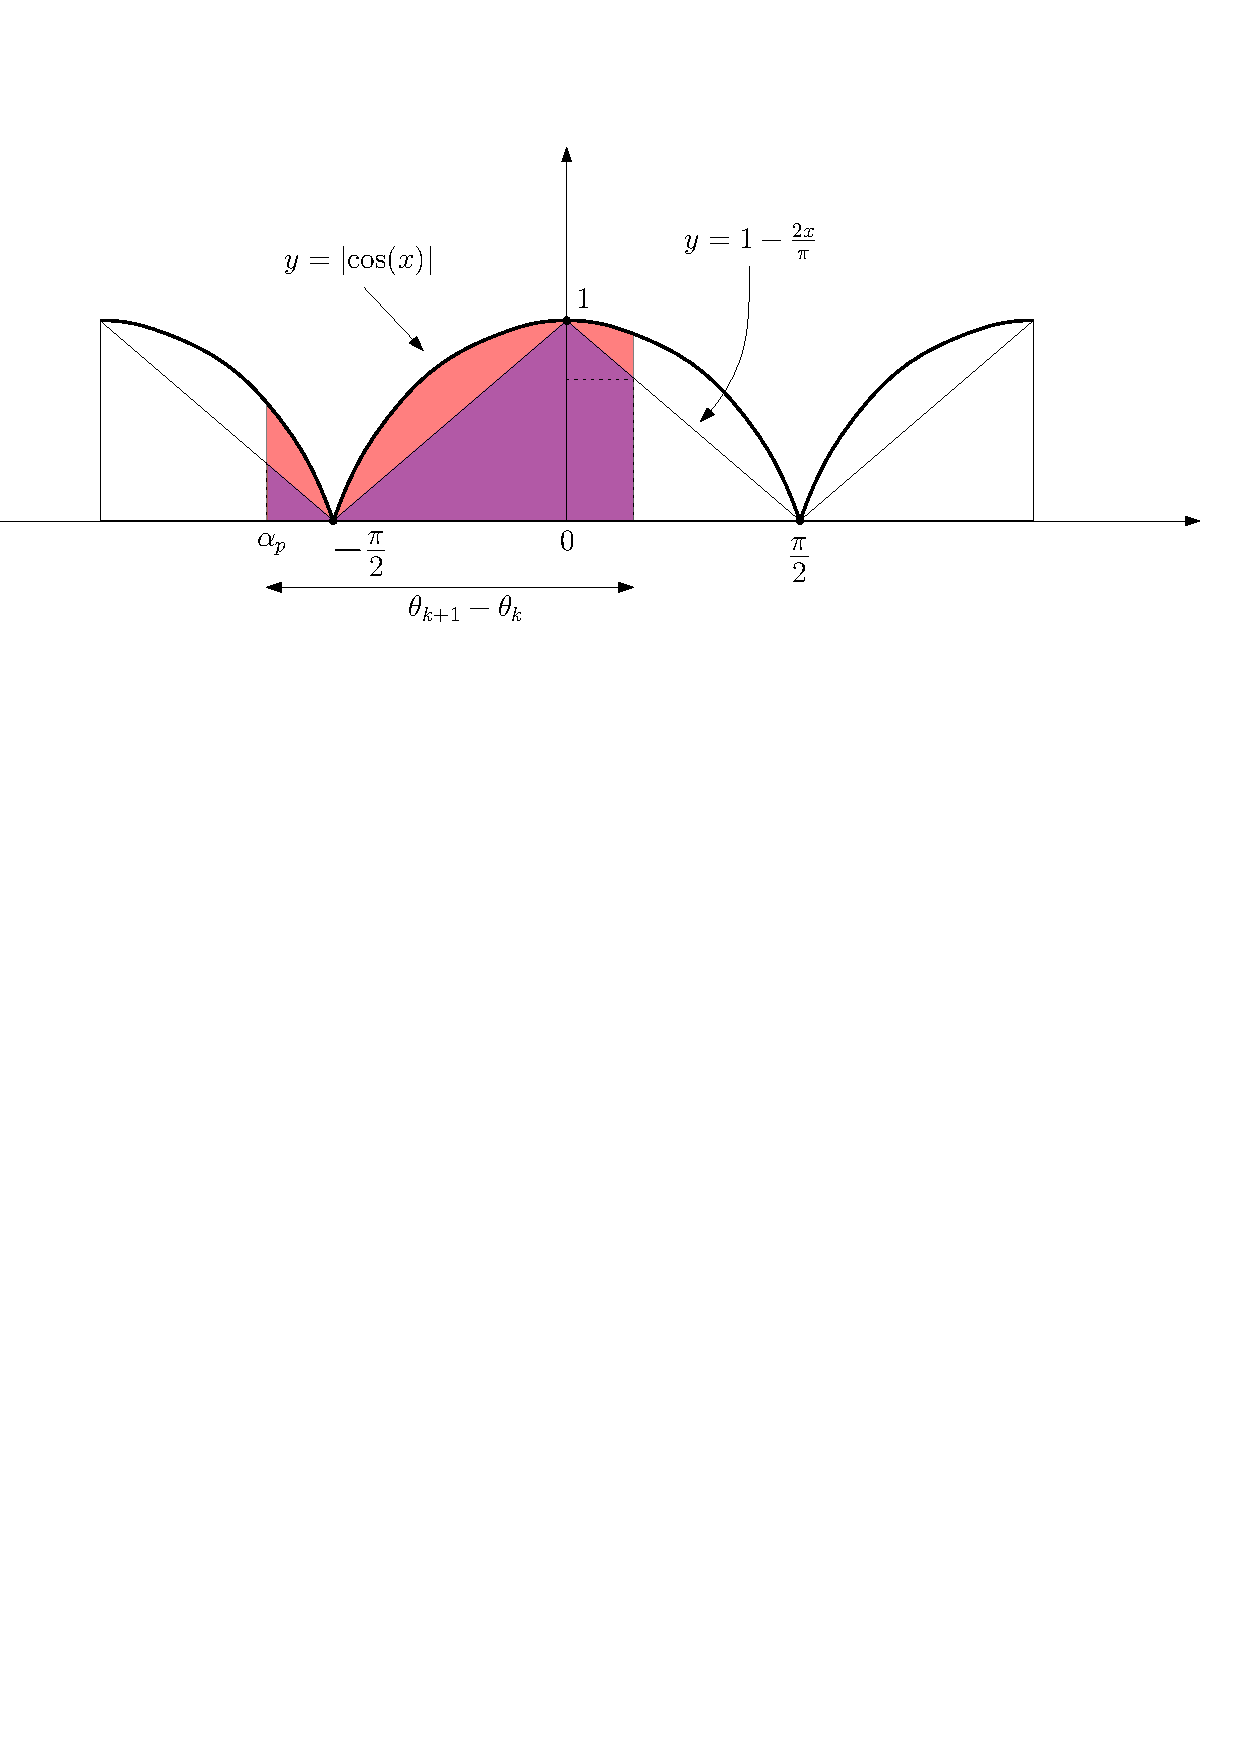
\includegraphics[width=15cm]{figures/cosineConcavity}
\caption[Concavity argument]{\label{fig:cosineConc}
The integral of $|{\rm cos}(\cdot)|$ has a lower bound that depends on the length of the integral support.
In particular, when $\theta_{k+1}-\theta_k\leq\pi$, this integral is more than $\frac{\left(\theta_{k+1}-\theta_k\right)^2}{2\pi}$ 
by the Cauchy-Schwarz inequality.}
\end{center}\end{figure}

We need to lower bound $\int_0^{\theta_{k+1}-\theta_k}|{\rm cos}\left(\alpha_p+\beta\right)|d\beta$.
Since $\theta_{k+1}-\theta_k\leq\pi$, one can show that this integral cannot be less than $\frac{\left(\theta_{k+1}-\theta_k\right)^2}{2\pi}$ 
using cosine concavity---see Figure~\ref{fig:cosineConc}. 
Hence, we now have the following lower bound:
 
\begin{align}
\int_{\theta_k}^{\theta_{k+1}} &\mathcal W(\mu_1^\theta+\mu_{2\Delta}^\theta,\mu_2^\theta+\mu_{1\Delta}^\theta)\ {\rm d}\theta
\geq \frac{\left(\theta_{k+1}-\theta_k\right)^2}{2\pi}\underset{p\in \dg_1\cup\pi_\Delta(\dg_2)}{\sum}\|p-\gamma(p)\|_2\nonumber\\
&\geq \frac{\left(\theta_{k+1}-\theta_k\right)^2}{2\pi}\underset{p\in \dg_1\cup\pi_\Delta(\dg_2)}{\sum}\|p-\gamma(p)\|_\infty\geq\
\frac{\left(\theta_{k+1}-\theta_k\right)^2}{2\pi}\underset{\substack{ p\notin \pi_\Delta(\dg_2) \\ {\rm\ or\ }\gamma(p)\notin\pi_\Delta(\dg_1)} }{\sum}\|p-\gamma(p)\|_\infty\nonumber\\
&\geq \frac{\left(\theta_{k+1}-\theta_k\right)^2}{2\pi}\distw{1}(\dg_1,\dg_2).
\nonumber
\end{align}

Let $\Theta=\left\{\theta_1=-\frac{\pi}{2},\theta_2,...,\theta_{|\Theta|}=\frac{\pi}{2}\right\}$. Then, one has:

\begin{align}
\SW&(\dg_1,\dg_2)=\frac{1}{\pi}\int_{-\frac{\pi}{2}}^{\frac{\pi}{2}} \mathcal W(\mu_1^\theta+\mu_{2\Delta}^\theta,\mu_2^\theta+\mu_{1\Delta}^\theta)\ {\rm d}\theta\nonumber\\
&=\frac{1}{\pi}\sum_{k=2}^{\card(\Theta)}\int_{\theta_{k-1}}^{\theta_{k}} \mathcal W(\mu_1^\theta+\mu_{2\Delta}^\theta,\mu_2^\theta+\mu_{1\Delta}^\theta)\ 	{\rm d}\theta\nonumber\\
&\geq \left(\sum_{k=2}^{\card(\Theta)}\left(\theta_{k}-\theta_{k-1}\right)^2\right)\frac{\distw{1}(\dg_1,\dg_2)}{2\pi^2} \nonumber\\
&\geq \frac{\pi^2}{\card(\Theta)-1}\frac{\distw{1}(\dg_1,\dg_2)}{2\pi^2}\text{ by the Cauchy-Schwarz inequality} \nonumber\\
&\geq \frac{\distw{1}(\dg_1,\dg_2)}{2M}
\nonumber
\end{align}

Hence, $\SW$ is discriminative.
\end{proof}

Theorems~\ref{th:stab} and~\ref{th:discr} allow us to show that $d_{\kSW}$, the distance induced by $\kSW$ in its RKHS,
is also equivalent to $\distw{1}$ in a broader sense: there exist continuous, positive and nondecreasing functions $g,h$ such that $g(0)=h(0)=0$
and $h\circ \distw{1}\leq d_{\kSW}\leq g\circ \distw{1}$.
 
\paragraph*{A weaker assumption.} The condition on the cardinalities of the persistence diagrams can be relaxed. 
Indeed, one can prove that the feature map $\Phi_{\kSW}$ induced by $\kSW$ 
is injective when the persistence diagrams are only assumed to be finite and bounded:

\begin{prop}\label{prop:inj}
%Let $X$ be the set of bounded and finite PDs.
The feature map $\Phi_{\kSW}$ %associated to $\kSW$ 
is continuous and injective with respect to $\distw{1}$ on $\SpfbD$.
\end{prop}	

\begin{proof}
Note that if the persistence diagrams have bounded cardinalities, Proposition~\ref{prop:inj} 
is an immediate consequence of Theorem~\ref{th:discr}.
One has that $\Phi_{\kSW}$ is continous since $d_{\kSW}$ is stable (cf Theorem~\ref{th:stab}).
Now, let $\dg_1,\dg_2\in \SpfbD$. %and $\mu_i,\mu_j$ be the two corresponding signed empirical measures
such that  $d_{\kSW}(\dg_1,\dg_2)=\|\Phi_{\kSW}(\dg_1)-\Phi_{\kSW}(\dg_2)\|=0$. 
We necessarily have $\SW(\dg_1,\dg_2)=0$.
Assume that $\distw{1}(\dg_1,\dg_2)>0$. 
Then, there must be a point $p$ in $\dg_1$ 
that is not in $\dg_2$.
The Sliced Wasserstein distance being $0$, there must be, for every $\theta\in\mathbb{S}_1$, 
a point $q_\theta$ in $\dg_2$ 
that has the same projection onto $L(\theta)$ as $p$: $\pi_\theta(q_\theta)=\pi_\theta(p)$, i.e. 
$q_\theta\in(\pi_\theta(p),p)$, the line defined by the pair $\pi_\theta(p),p$. 
All these lines $(\pi_\theta(p),p)$ intersect at $p\neq q_\theta$.
Thus, $q_{\theta_1}\neq q_{\theta_2}$ for any $\theta_1\neq \theta_2$, hence $\dg_2$
includes an infinite number of points,
which is impossible since $\dg_2\in\SpfbD$. Thus, $\distw{1}(\dg_1,\dg_2)=0$ and $\Phi_{\kSW}$ is injective. 
\end{proof}

In particular, $\kSW$ can be turned into a universal kernel by considering ${\rm exp}(\kSW)$  (cf Theorem~1 in~\cite{Kwitt15}).
This can be useful in a variety of tasks, including tests on distributions of persistence diagrams.
%Note also that $\kSW$ is not additive.

\subsection{Computation}
\label{sec:comput}

\paragraph*{Approximate computation.} In practice, $\kSW$ can be approximated in $O(N{\rm log}(N))$
time using Algorithm~\ref{alg:aksw}. This algorithm first samples $M$ directions
in the half-circle $\mathbb{S}^+_1$; it then computes, for
each sample $\theta_i$ and for each persistence diagram $\dg$, the scalar
products between the points of $\dg$ and $\theta_i$, and then sorts them in a
vector $V_{\theta_i}(\dg)$. Finally, the $\ell_1$-norm between the vectors 
%gives the 
%1D Wasserstein distance $w_\infty^1$ along $L(\theta_i)$; 
%this value 
is averaged over the sampled directions:
%\begin{align*}
$\SW_M(\dg_1,\dg_2)%&:=\frac 1M \sum_{i=1}^M w_\infty^1 (\dg_1^{\theta_i},\dg_2^{\theta_i})\nonumber \\
%&
=\frac 1M \sum_{i=1}^M \|V_{\theta_i}(\dg_1)-V_{\theta_i}(\dg_2)\|_1.$
%\nonumber
%\end{align*}
Note that one can easily adapt the proof of Lemma~\ref{lem:nd} to show that $\SW_M$ 
%this approximation 
is conditionally negative semi-definite
%:={\rm e}\left(-\frac{{\rm SW}_M(\dg_1,\dg_2)}{2\sigma^2}\right)$ 
by using the linearity of the sum. Hence, this approximation remains a kernel.
%If there are $M$ samples of $\mathbb{S}_1^+$ and 
If the two persistence diagrams have cardinalities bounded by $N$,
then the running time of this procedure is $O(MN{\rm log}(N))$. This approximation of $\kSW$  
is useful since, as shown in Section~\ref{sec:expe}, we can observe empirically that just a 
few directions are sufficient to get good classification accuracies.

\begin{algorithm}
\caption{Approximate computation of $\SW$}
\label{alg:aksw}
\begin{algorithmic}
\STATE {\bfseries Input:} $\dg_1=\{p^1_1,\cdots,p^1_{N_1}\}$, $\dg_2=\{p^2_1,\cdots,p^2_{N_2}\}, M$.
\STATE Add $\pi_\Delta(\dg_1)$ to $\dg_2$ and vice-versa.
\STATE Let $\SW=0$; $\theta=-\pi/2$; $s=\pi/M$;
\FOR{$i=1,\cdots,M$}
	\STATE Store the products $\langle p_k^1,\theta\rangle$ in an array $V_1$;
	\STATE Store the
 products $\langle p_k^2,\theta\rangle$ in an array $V_2$;
	\STATE Sort $V_1$ and $V_2$ in ascending order;
	\STATE $\SW=\SW+s \|V_1-V_2\|_1$;
	\STATE $\theta= \theta + s$;
\ENDFOR
\STATE {\bfseries Output:} $(1/\pi)\SW$;
\end{algorithmic}
\end{algorithm}  

\paragraph*{Exact computation.} A persistence diagram is said to be in {\em general position} if it has no triple of aligned points.  
If the persistence diagrams have cardinalities bounded by $N$, then the exact kernel computation for persistence diagrams in general 
position can be done in $O(N^2{\rm log}(N))$ time with 
Algorithm~\ref{alg:ksw}. In practice, given $\dg_1$ and $\dg_2$, we slightly modify them with infinitesimally small random perturbations, so that
the resulting persistence diagrams 
$\tilde{\dg}_1$ and $\tilde{\dg}_2$ are in general position. We then approximate 
$\kSW(\dg_1,\dg_2)$ arbitrarily well with $\kSW(\tilde{\dg}_1,\tilde{\dg}_2)$.	

\begin{algorithm}
\caption{Exact computation of $\SW$}\label{alg:ksw}
%\KwIn{$\dg_1=\{p^1_1\ ...\ p^1_{N_1}\}$, % with $\card(\dg_1)=N_1$, 
\KwIn{$\dg_1=\{p^1_1,\cdots,p^1_{N_1}\}$ with $|\dg_1|=N_1$, $\dg_2=\{p^2_1,\cdots,p^2_{N_2}\}$ with $|\dg_2|=N_2$}
Let $\Theta^1=[],\Theta^2=[],V_1=[],V_2=[]$, $B_1=[[]\ ...\ []]$, $B_2=[[]\ ...\ []]$, $\SW=0$;\\
\For{$i=1,\cdots,N_1$}{
    Add $p^2_{N_2+i}=\pi_\Delta(p^1_i)$ to $\dg_2$;
  }
\For{$i=1,\cdots,N_2$}{
    Add $p^1_{N_1+i}=\pi_\Delta(p^2_i)$ to $\dg_1$;
  }
\For{$i=1,2$}{
  \For{$j=1,\cdots,N_1+N_2-1$}{
    \For{$k=j+1,\cdots,N_1+N_2$}{
      Add $\angle \left[p^i_j-p^i_k\right]^\perp \in \left[-\frac{\pi}{2},\frac{\pi}{2}\right]$ to $\Theta^i$;
    }
  }
  Sort $A^i$ in ascending order;\\
  \For{$j=1,\cdots,N_1+N_2$}{
    Add $\langle p_j^i,[0,-1]\rangle$ to $V_i$;
  }
  Sort $V_i$ in ascending order;\\
  Let $f_i:p^i_j\mapsto{\rm position\ of\ }\left(p_j^i,-\frac{\pi}{2}\right){\rm\ in\ }V_i$; \\
  \For{$j=1,\cdots,(N_1+N_2)(N_1+N_2-1)/2$}{
    Let $k_1,k_2$ such that $\Theta^i[j]=\angle \left[p^i_{k_1}-p^i_{k_2}\right]^\perp$;\\
    Add $\left(p^i_{k_1},\Theta^i[j]\right)$ to $B_i\left[f_i(p^i_{k_1})\right]$; Add $\left(p^i_{k_2},\Theta^i[j]\right)$ to $B_i\left[f_i(p^i_{k_2})\right]$;\\
    Swap $f_i(p^i_{k_1})$ and $f_i(p^i_{k_2})$;
  }
  \For{$j=1,\cdots,N_1+N_2$}{
    Add $\left(p^i_j,\frac{\pi}{2}\right)$ to $B_i\left[f_i(p_j^i)\right];$
  }
}
\For{$i=1,\cdots,N_1+N_2$}{
  Let $k_1=0$, $k_2=0$;\\
  Let $\theta_m=-\frac{\pi}{2}$ and $\theta_M={\rm min}\{B_1[i][k_1]_2,B_2[i][k_2]_2\}$;\\
  \While{$\theta_m\neq \frac{\pi}{2}$}{
  $\SW = \SW+\|B_1[i][k_1]_1-B_2[i][k_2]_1\|_2\int_{0}^{\theta_M-\theta_m}{\rm cos}(\angle\left(B_1[i][k_1]_1-B_2[i][k_2]_1,\theta_m\right)+\theta){\rm d}\theta$;\\
  $\theta_m=\theta_M$;\\
  {\bf{\text if }} $\theta_M==B_1[i][k_1]_2$ {\bf {\text then }}$k_1=k_1+1$; {\bf{\text else }}$k_2=k_2+1$;\\
  $\theta_M={\rm min}\{B_1[i][k_1]_2,B_2[i][k_2]_2\}$;
  }
}
{\bf{\text return }}$\frac{1}{\pi}\SW$;
\end{algorithm}  



\subsection{Experiments}
\label{sec:expe}

In this section, we compare $\kSW$ to $\kPSS$ and $\kPWG$ on 
several benchmark applications for which persistence diagrams have been proven useful. 
We compare these kernels in terms of classification 
accuracies and computational cost. We review first our experimental setting, and review these tasks one by one.

\paragraph*{Experimental setting.}
We implemented and used C++ code to compute kernel values in the Gudhi C++ library~\cite{gudhi:Kernels}. These values are then handled with the LIBSVM~\cite{Chang01} implementation of $C$-SVM, and results are averaged over 10 runs
on a 2.4GHz Intel Xeon E5530 Quad Core.
The cost factor $C$ is cross-validated in the following grid: $\{0.001, 0.01,0.1, 1,10,100,1000\}$.
Table~\ref{table:sum} summarizes the properties of the datasets we consider, namely number of labels, as well as training and test instances 
for each task. Figure~\ref{fig:taskltm} and \ref{fig:task2} illustrate how we use persistence diagrams to represent complex data.
We first describe the two baselines we considered, along with their parameterization, followed by our proposal.

\begin{table}[t]
\vskip 0.15in
\begin{center}
\begin{small}
\begin{sc}
\begin{tabular}{|l|c|c|c|}
\hline
 Task &        Training &                               Test &                       Labels \\
\hline
Orbit &        175 &                                    75 &                         5  \\
Texture &      240 &                                    240 &                        24  \\
Human &        415 &                                    1618 &                       8 \\
Airplane &     300 &                                    980 &                        4 \\
Ant &          364 &                                    1141 &                       5 \\
Bird &         257 &                                    832 &                        4 \\
FourLeg &      438 &                                    1097 &                       6 \\
Octopus &      334 &                                    1447 &                       2 \\
Fish &         304 &                                    905 &                        3 \\
\hline          
\end{tabular}
\end{sc}
\end{small}
\caption{\label{table:sum} Number of instances in the training set, the test set and number of labels.}
\end{center}
\vskip -0.1in
\end{table}

\begin{table}[t]
\vskip 0.15in
\begin{center}
\begin{small}
\begin{sc}

\begin{tabular}{|l|lll|}
\hline 
Task &         $\kPSS$ ($10^{-3}$)&    $\kPWG$ (1000) &                   $\kSW$ (6)                                  \\
\hline 
Orbit &        $63.6\pm1.2$ &          $77.7\pm1.2$ &                     ${\bf 83.7}\pm0.5$                           \\        
Texture &      ${\bf 98.8}\pm 0.0$ &   $95.8\pm0.0$ &                     $96.1\pm0.4$                          \\                                           
\hline 
Task &         $\kPSS$ &               $\kPWG$ &                          $\kSW$                           \\
\hline 
Human &        $68.5\pm2.0$ &          $64.2\pm1.2$ &                     ${\bf 74.0}\pm0.2 $ \\
Airplane &     $65.4\pm2.4$ &          $61.3\pm2.9$ &                     ${\bf 72.6}\pm0.2$  \\
Ant &          $86.3\pm1.0$ &          $87.4\pm0.5$ &                     ${\bf 92.3}\pm0.2$  \\
Bird &         $67.7\pm1.8$ &          ${\bf72.0}\pm1.2$ &                $67.0\pm0.5$  \\
FourLeg &      $67.0\pm2.5$ &          $64.0\pm0.6$ &                     ${\bf73.0}\pm0.4$ \\
Octopus &      $77.6\pm1.0$ &          $78.6\pm1.3$ &                     ${\bf85.2}\pm0.5$  \\
Fish &         $76.1\pm1.6$ &          ${\bf79.8}\pm0.5$ &                $75.0\pm0.4$ \\
\hline                                                            
\end{tabular}
\end{sc}
\end{small}

\caption{\label{table:Acc} Classification accuracies (\%) for the benchmark applications.}
\end{center}
\vskip -0.1in
\end{table}

\begin{table}[t]
\vskip 0.15in
\begin{center}
\begin{small}
\begin{sc}
\begin{tabular}{|l|llll|}
\hline 
Task &         $\kPSS$ ($10^{-3}$) &  $\kPWG$ (1000) &    $\kSW$ (6) &         \\
\hline 
Orbit &        $N(124\pm8.4)$ &       $N(144\pm14)$ &     $415\pm7.9+NC$ &                     \\        
Texture &      $N(165\pm27)$ &        $N(101\pm9.6)$ &    $482\pm68+NC$ &                      \\                                           
\hline 
Task &         $\kPSS$ &              $\kPWG$ &           $\kSW$ &           $\kSW$ (10) \\
\hline 
Human &        $N(29\pm0.3)$ &        $N(318\pm22)$ &     $2270\pm336+NC$ &  $107\pm14+NC$ \\
Airplane &     $N(0.8\pm0.03)$ &      $N(5.6\pm0.02)$ &   $44\pm5.4+NC$ &    $10\pm1.6+NC$ \\
Ant &          $N(1.7\pm0.01)$ &      $N(12\pm0.5)$ &     $92\pm2.8+NC$ &    $16\pm0.4+NC$ \\
Bird &         $N(0.5\pm0.01)$ &      $N(3.6\pm0.02)$ &   $27\pm1.6+NC$ &    $6.6\pm0.8+NC$ \\
FourLeg &      $N(10\pm0.07)$ &       $N(113\pm13)$ &     $604\pm25+NC$ &    $52\pm3.2+NC$ \\
Octopus &      $N(1.4\pm0.01)$ &      $N(11\pm0.8)$ &     $75\pm1.4+NC$ &    $14\pm2.1+NC$ \\
Fish &         $N(1.2\pm0.004)$ &     $N(9.6\pm0.03)$ &   $72\pm4.8+NC$ &    $12\pm1.1+NC$ \\
\hline                                                            
\end{tabular}

\end{sc}
\end{small}
\caption{\label{table:Gram} Gram matrices computation time (s) for the benchmark applications.
As explained in the text, $N$ represents the size of the set of possible parameters, and we have $N=13$ for $\kPSS$, 
$N=5\times5\times5=125$ for $\kPWG$ and $N=3\times5=15$ for $\kSW$. $C$ is a constant that depends only on the
training size. In all our applications, it is less than $0.1$s.}
\end{center}
\vskip -0.1in
\end{table}

\begin{figure*}[t] 
\centering
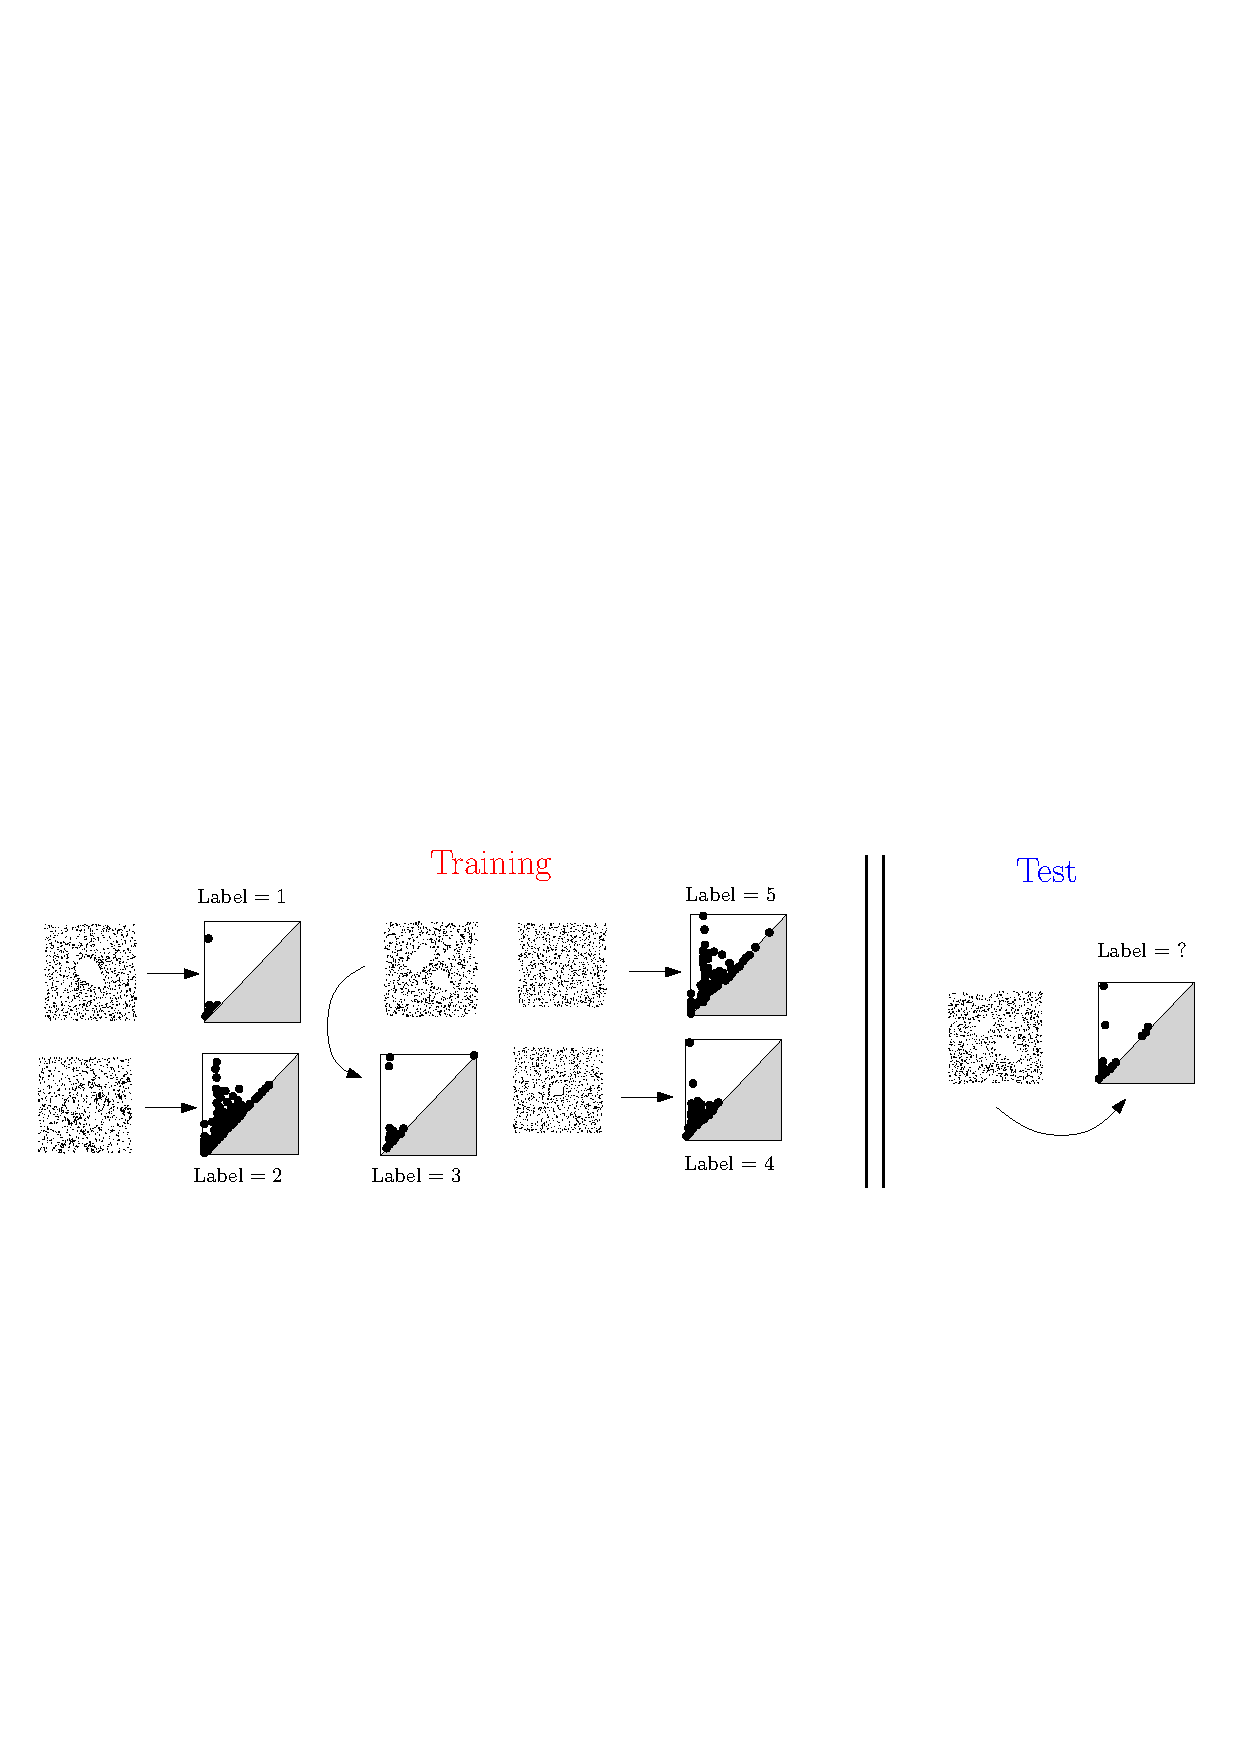
\includegraphics[width=0.98\textwidth]{figures/ltm/taskltm}
\caption[Orbit recognition]{\label{fig:taskltm} Sketch of the orbit recognition task. Each parameter $r$ in the 5 possible choices
leads to a specific behavior of the orbit. 
The goal is to recover parameters from the persistent homology of orbits in the test set.}
\end{figure*}

\begin{figure*}[t] 
\centering
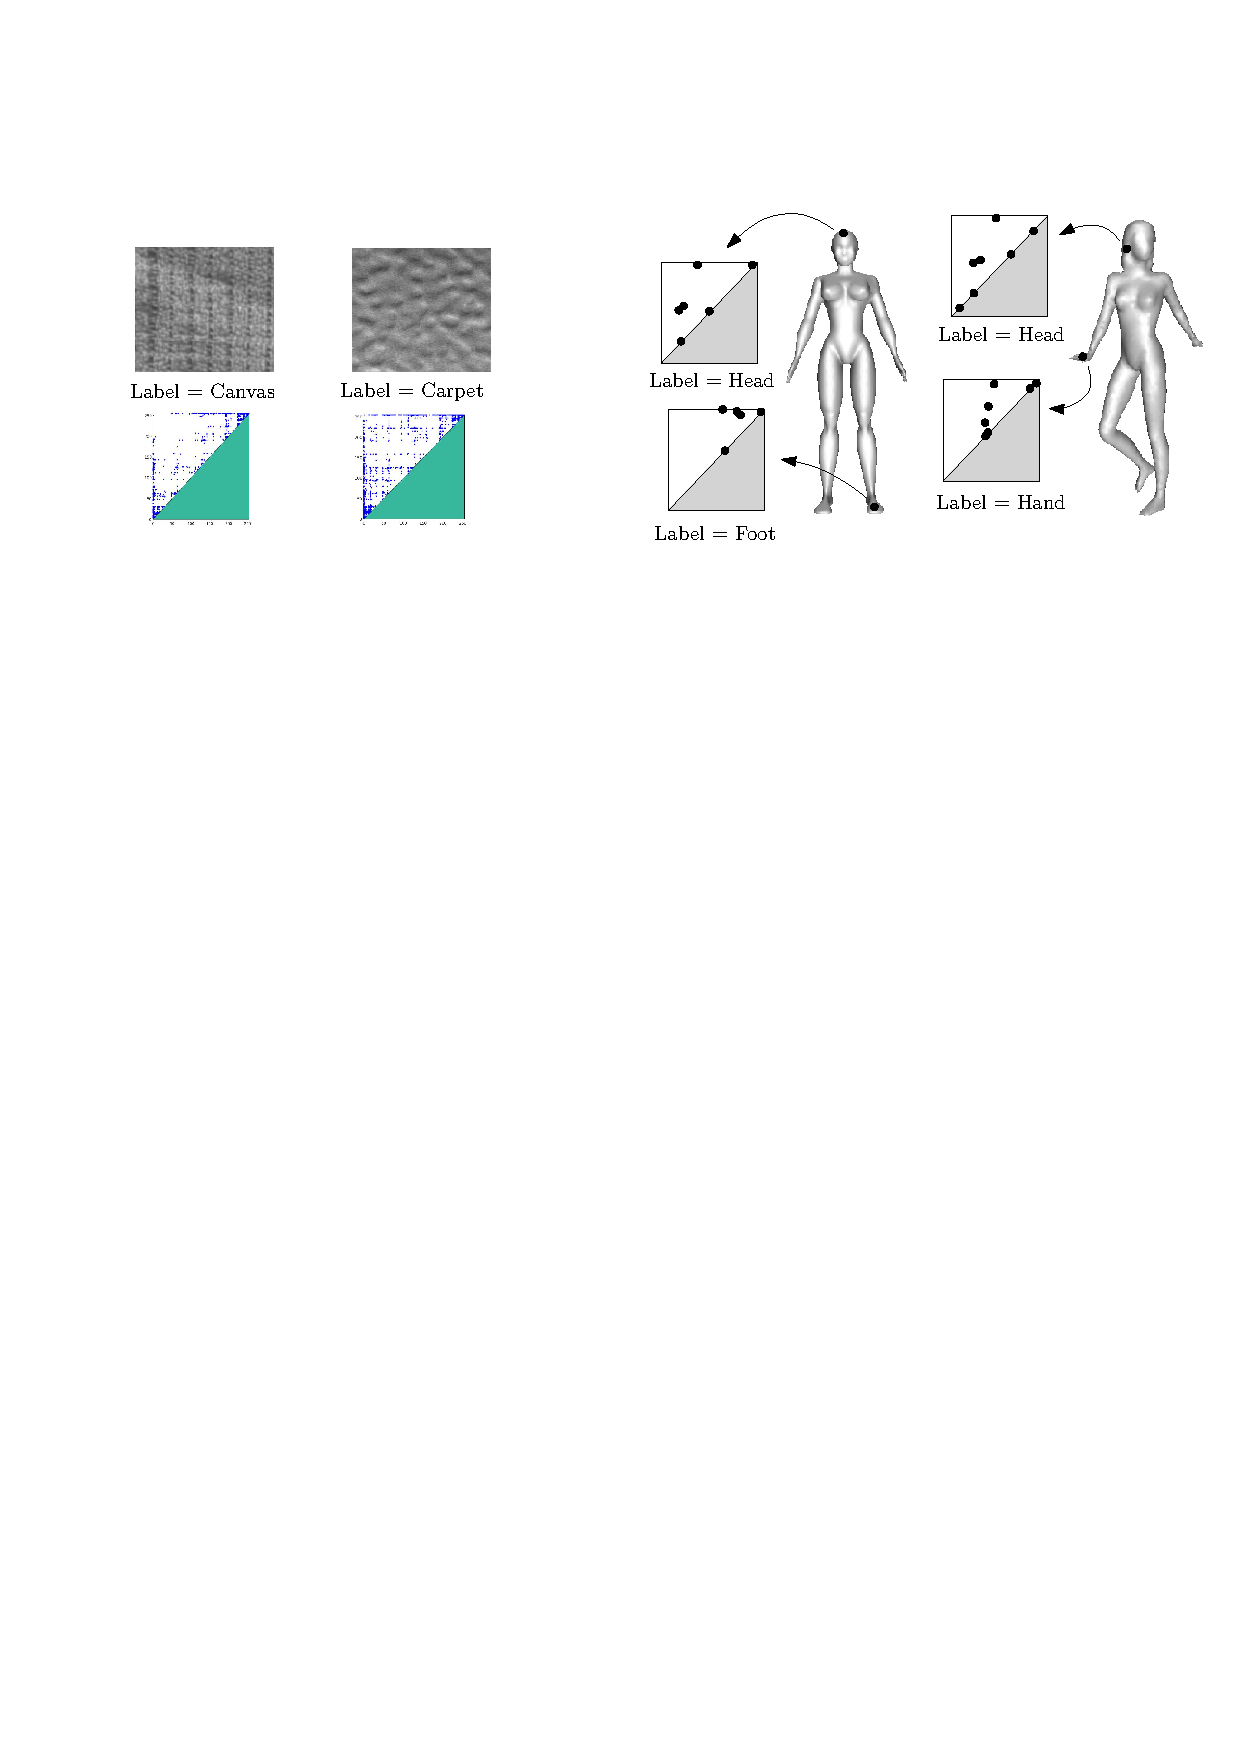
\includegraphics[width=0.98\textwidth]{figures/task2}
\caption[Texture and 3D point classification]{\label{fig:task2} Examples of persistence diagrams computed on texture images from the \emph{OUTEX00000} dataset
and persistence diagrams computed from points on 3D shapes. One can see that corresponding points in different shapes have
similar persistence diagrams.}
\end{figure*}

\begin{figure}\centering
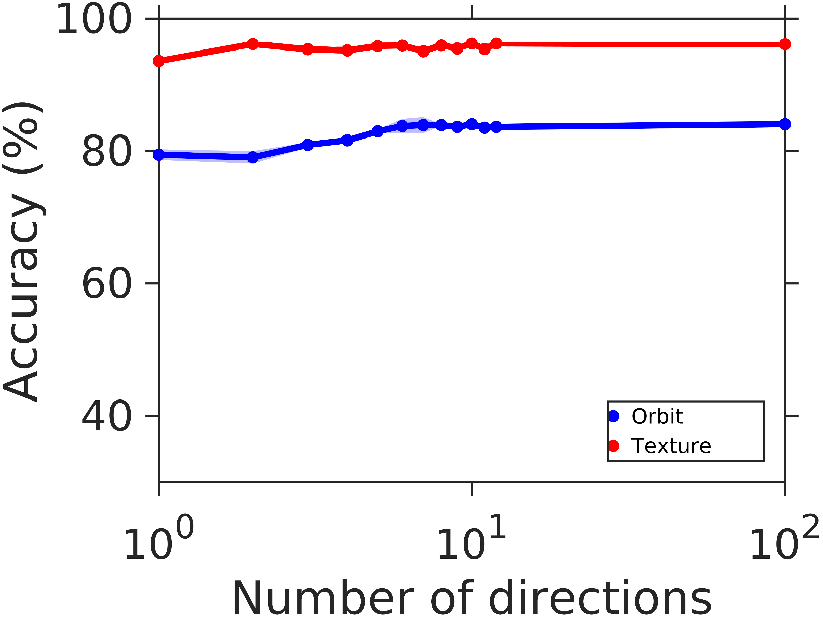
\includegraphics[width=7.5cm]{figures/accVSdir.pdf}\ \ 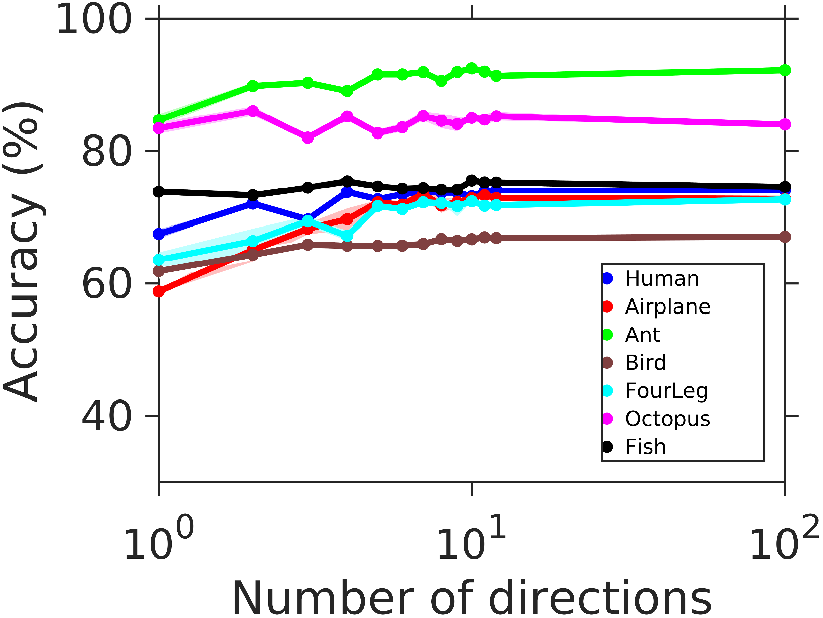
\includegraphics[width=7.5cm]{figures/accVSdirprinceton.pdf} \\
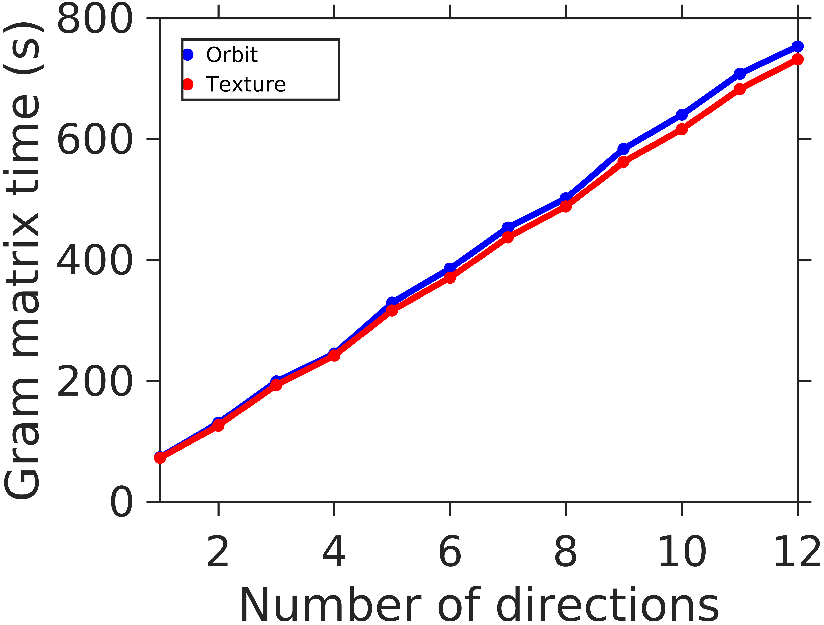
\includegraphics[width=7.5cm]{figures/timeVSdir.pdf} \ \ 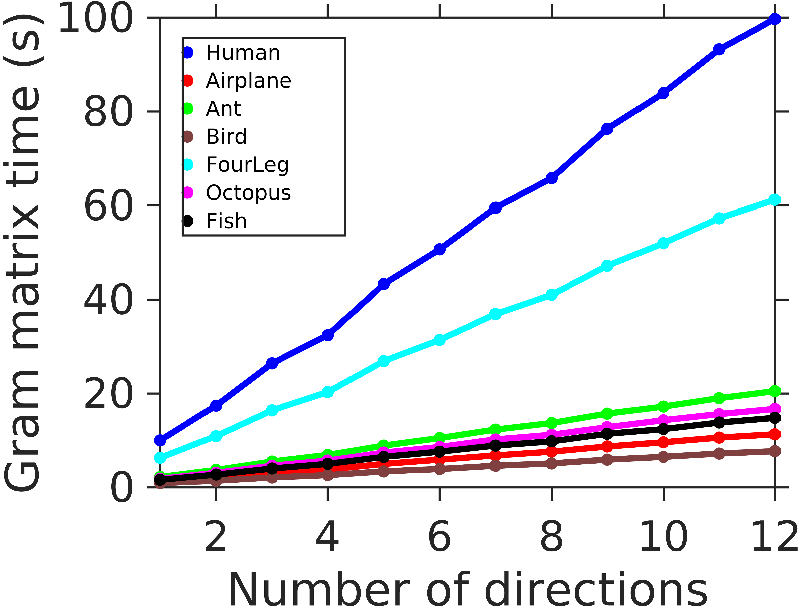
\includegraphics[width=7.5cm]{figures/timeVSdirprinceton.pdf} \\
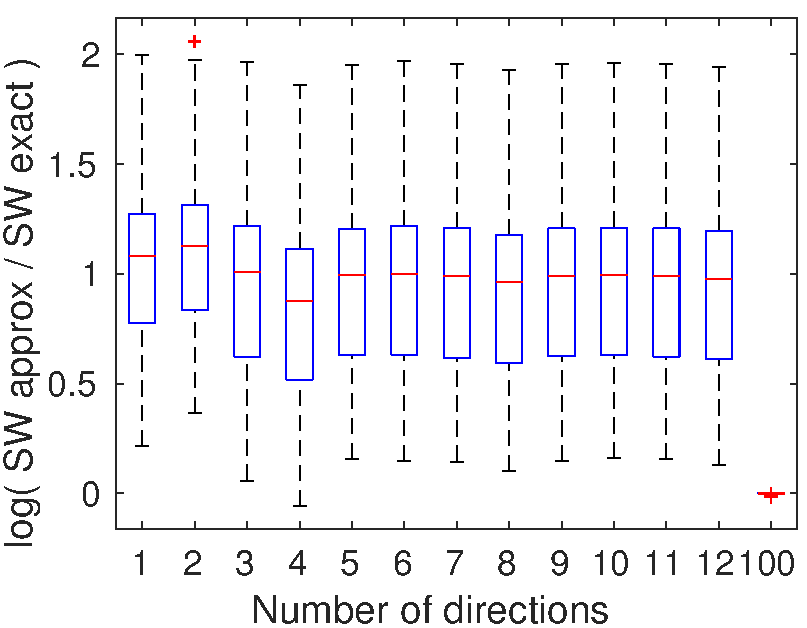
\includegraphics[width=7.5cm]{figures/ratiooutex.pdf}\ \ 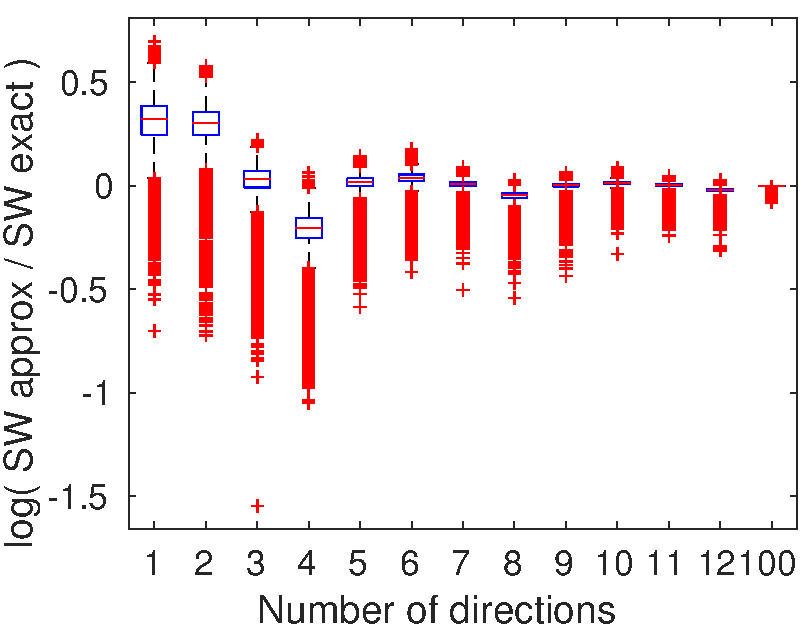
\includegraphics[width=7.5cm]{figures/ratioprinceton.pdf}
\caption[Accuracy and training time dependences on direction number]{\label{fig:plots} The first column corresponds to the orbit recognition and the texture classification while the second
column corresponds to 3D shape segmentation. 
On each column, the first row shows the dependence of the accuracy on the number of directions,
the second row shows the dependence of a single Gram matrix computation time, and the third row
shows the dependence of the ratio of the approximation of $\SW$ and the exact $\SW$.
Since the box plot of the ratio for orbit recognition is very similar to that of 3D shape segmentation,
we only give the box plot of texture classification in the first column. }
\end{figure}


\paragraph*{PSS.} The {\em Persistence Scale Space} kernel $\kPSS$~\cite{Reininghaus15} is
defined as the scalar product of the two solutions of the heat diffusion equation
with initial Dirac sources located at the points of the persistence diagram. It has the following closed form expression:
$$\kPSS(\dg_1,\dg_2)=\frac{1}{8\pi t}\sum_{p\in \dg_1}\sum_{q\in \dg_2} {\rm exp}\left(-\frac{\|p-q\|^2}{8t}\right) 
- {\rm exp}\left(-\frac{\|p-\bar q\|^2}{8t}\right),$$
where $\bar q=(y,x)$ is the symmetric of $q=(x,y)$ along the diagonal.
Since there is no clear heuristic on how to tune $t$, this parameter is chosen in the applications 
by ten-fold cross-validation with random 50\%-50\%
training-test splits and with the following set of $N_{\rm PSS}=13$ values: $0.001$, $0.005$, $0.01$, $0.05$, 
$0.1$, $0.5$, $1$, $5$, $10$, $50$, $100$, $500$ and $1000$. 

\paragraph*{PWG.} Let $K,p>0$ and $\dg_1$ and $\dg_2$ be two persistence diagrams.
Let $k_\rho$ be the Gaussian kernel with parameter $\rho >0$.
Let $\mathcal{H}_\rho$ be the RKHS associated to $k_\rho$.
Let $\mu_1=\sum_{x\in D_1}{\rm arctan}(K{\rm pers}(x)^p)k_\rho(\cdot,x)\in\mathcal{H}_\rho$ 
be the kernel mean embedding of $\dg_1$ weigthed by the diagonal distances.
Let $\mu_2$ be defined similarly. Let $\tau >0$.
The {\em Persistence Weighted Gaussian} kernel $\kPWG$~\cite{Kusano16, Kusano17} is
defined as the Gaussian kernel with parameter $\tau$ on $\mathcal{H}_\rho$:
$$\kPWG(\dg_1,\dg_2)={\rm exp}\left(-\frac{\|\mu_1-\mu_2\|_{\mathcal{H}_\rho}}{2\tau^2}\right).$$
The authors in~\cite{Kusano16} provide heuristics to compute $K$, $\rho$ and $\tau$
and give a rule of thumb to tune $p$. Hence, in the applications we select $p$ according to the rule of thumb, and
 we use ten-fold cross-validation with random 50\%-50\% training-test splits to chose $K$, $\rho$ and $\tau$. 
The ranges of possible values is obtained 
by multiplying the values computed with the heuristics
with the following range of $5$ factors: $0.01$, $0.1$, $1$, $10$ and $100$,
leading to $N_{\rm PWG}=5\times 5\times 5=125$ different sets of parameters.

\paragraph*{Parameters for $\kSW$.} The kernel we propose has only one parameter, the bandwidth $\sigma$ in Eq.~\ref{eq:kSW}, 
which we choose
using ten-fold cross-validation with random 50\%-50\% training-test splits. 
The range of possible values is obtained by computing the squareroot of the median, the first and the last deciles 
of all $\SW(\dg_i,\dg_j)$ in the training set,
then by multiplying these values by the following range of $5$ factors: $0.01$, $0.1$, $1$, $10$ and $100$, 
leading to $N_{\rm SW}=5\times 3= 15$ possible values. 


\paragraph*{Parameter Tuning.} The bandwidth of $\kSW$ is, in practice, easier to tune than the parameters of its two competitors
when using grid search. Indeed, as is the case for all infinitely divisible kernels, the Gram matrix does not need to be 
recomputed for each choice of $\sigma$, since it only suffices to compute all the Sliced Wasserstein distances between persistence diagrams
in the training set once. On the contrary, neither $\kPSS$ nor $\kPWG$ share this property, and require recomputations for each hyperparameter choice.
Note however that this improvement may no longer hold if one uses other methods to tune parameters.  
For instance, using $\kPWG$ without cross-validation is possible with the heuristics given by the authors in~\cite{Kusano16}, 
and leads to smaller training times, but also to worse accuracies. 



\paragraph*{3D shape segmentation.}
Our first task is the same as in Section~\ref{sec:VectorExpe}, namely we produce point classifiers for 3D shapes.
%follows that presented in~\cite{Carriere15a}.

{\bf Data.}  We use some categories of the mesh segmentation benchmark of Chen et al.~\cite{Chen09},
which contains 3D shapes classified in several categories (``airplane'', ``human'', ``ant''...).
For each category, our goal is to design a classifier that can assign, to each point in the shape,
a label that describes the relative location of that point in the shape. For instance, possible labels are, for the human category, 
``head'', ``torso'', ``arm''...
To train classifiers, we compute a persistence diagram per point using the geodesic distance function 
to this point---we give more details on this persistence diagram in Section~\ref{sec:VectorExpe}.
%We use 1-dimensional persistent homology (0-dimensional would not be informative since the shapes are connected,
%leading to solely one point with coordinates $(0,+\infty)$ per PD). 
For each category, the training set contains one hundredth of the points of the first five 3D shapes,
and the test set contains one hundredth of the points of the remaining shapes in that category. Points in
training and test sets are evenly sampled. See Figure~\ref{fig:task2}.
Here, we focus on comparison between persistence diagrams, and not
on achieving state-of-the-art results. We show in Section~\ref{sec:VectorExpe} that 
persistence diagrams bring complementary information
to classical descriptors in this task, hence reinforcing their discriminative power with appropriate kernels is of great interest.
Finally, since data points are in $\R^3$, we set the $p$ parameter of $\kPWG$ to $5$. 

{\bf Results.} Classification accuracies are given in Table~\ref{table:Acc}.
For most categories, $\kSW$ outperforms competing kernels by a significant margin.
The variance of the results over the run is also less than that of its competitors. 
However, training times are not better in general. 
Hence, we also provide the results for an approximation of $\kSW$ with $10$ directions.
As one can see from Table~\ref{table:Acc} and from Figure~\ref{fig:plots}, this approximation leaves the accuracies almost unchanged, 
while the training times become comparable with the ones of the other competitors. Moreover, 
according to Figure~\ref{fig:plots}, using even less directions
would slightly decrease the accuracies, but still outperform the competitors performances,
while decreasing even more the training times. 


\paragraph*{Orbit recognition.}
In our second experiment, we use synthetized data.
The goal is to retrieve parameters of dynamical system orbits,
following an experiment proposed in~\cite{Adams17}.

{\bf Data.} We study the {\em linked twist map}, a discrete dynamical system modeling
fluid flow. It was used in~\cite{Hertzsch07} to model flows in DNA microarrays.
Its orbits can be computed given a parameter $r>0$ and
initial positions $(x_0,y_0)\in[0,1]\times[0,1]$ as follows:

\[\left\{\begin{array}{l} x_{n+1} = x_n + ry_n(1-y_n)\ \ \ \ \ \ \ \ \ \ \ {\rm mod}\ 1 \\ y_{n+1} = y_n + rx_{n+1}(1-x_{n+1})\ \ \ {\rm mod}\ 1 \end{array}\right.\]

Depending on the values of $r$, the orbits may exhibit very different behaviors. For instance,
as one can see in Figure~\ref{fig:taskltm}, when $r$ is 3.5, there seems to be no interesting topological features
in the orbit, while voids form for $r$ parameters around 4.3.
Following~\cite{Adams17}, we use 5 different parameters $r=2.5,3.5,4,4.1,4.3$, that act as labels.
For each parameter, we generate 100 orbits with 1000 points and random initial positions. We then compute
the persistence diagrams of the distance functions to the point clouds with the Gudhi C++ library~\cite{gudhi:PersistentCohomology} and we use them (in all homological dimensions) 
to produce an orbit classifier
that predicts the parameter values, by training over a 70\%-30\% training-test split of the data.
Since data points are in $\R^2$, we set the $p$ parameter of $\kPWG$ to $4$.

{\bf Results.} Since the persistence diagrams contain thousands of points, we use kernel approximations
to speed up the computation of the Gram matrices.
In order for the approximation error to be bounded by $10^{-3}$, 
we use an approximation of $\kSW$ with $6$ directions (as one can see from Figure~\ref{fig:plots}, 
this has a small impact on the accuracy), we approximate $\kPWG$ with $1000$ random Fourier features~\cite{Rahimi08},
and we approximate $\kPSS$ using Fast Gauss Transform~\cite{Morariu09}
with a normalized error of $10^{-10}$. 
One can see from Table~\ref{table:Acc} that the accuracy is increased a lot with $\kSW$.
Concerning training times, there is also a large improvement since we tune the parameters with grid search. 
Indeed, each Gram matrix needs not be recomputed for each parameter when using $\kSW$.

\paragraph*{Texture classification.}
Our last experiment is inspired from~\cite{Reininghaus15} and~\cite{Li14}. 
We use the OUTEX00000 data base~\cite{Ojala02} for texture classification. 

{\bf Data.} Persistence diagrams are obtained for each texture image by computing first the sign component of CLBP descriptors~\cite{Guo10} 
with radius $R=1$ and $P=8$ neighbors for each image,
and then compute the persistent homology of this descriptor using the Gudhi C++ library~\cite{gudhi:CubicalComplex}. 
See Figure~\ref{fig:task2}.
Note that, contrary to the experiment of~\cite{Reininghaus15}, we do not downsample the images to $32\times 32$ images,
but keep the original $128\times128$ images. 
Following~\cite{Reininghaus15}, we restrict the focus to 0-dimensional persistent homology.
We also use the first 50\%-50\% training-test split given in the database to produce classifiers. 
Since data points are in $\R^2$, we set the $p$ parameter of $\kPWG$ to $4$. 

{\bf Results.} We use the same approximation procedure as in the previous experiment.
According to Figure~\ref{fig:plots}, even though the approximation of $\SW$ is rough,
this has again a small impact on the accuracy, while reducing the training time by a significant margin.
As one can see from Table~\ref{table:Acc}, 
using $\kPSS$ leads to almost state-of-the-art results~\cite{Ojala02, Guo10},
closely followed by the accuracies of $\kSW$ and $\kPWG$.
The best timing is given by $\kSW$, again because we use grid search. 
Hence, $\kSW$ almost achieves the best result, and its training time is
better than the ones of its competitors, due to the grid search parameter tuning.




\paragraph*{Metric Distortion.} 
To illustrate the equivalence theorem, we also show in Figure~\ref{fig:Airplanedistances} 
a scatter plot where each point represents the comparison of two persistence diagrams taken from the Airplane segmentation data set. 
Similar plots can be obtained with the other datasets considered here.
For all points, the x-axis quantifies the 1-Wasserstein distance $\distw{1}$ for that pair,
while the y-axis is the logarithm of the RKHS distance induced by either $\kSW$, $\kPSS$, $\kPWG$ 
or a Gaussian kernel directly applied to $\distw{1}$, to obtain comparable quantities. 
We use the parameters given by the cross-validation procedure described above.
One can see that the distances induced by $\kSW$ are less spread than the others,
suggesting that the metric induced by $\kSW$ is more discriminative.
Moreover the distances given by $\kSW$ and the Gaussian kernel on $\distw{1}$ exhibit the same behavior, 
suggesting that $\kSW$ is the best natural equivalent of a Gaussian kernel for persistence diagrams. 

\begin{figure}\centering
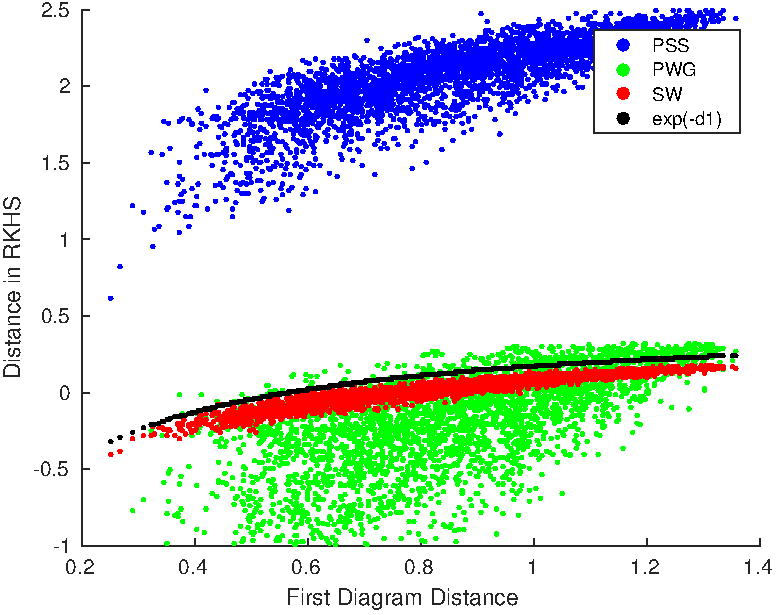
\includegraphics[width=8cm]{figures/distance/distances.pdf}
\caption[Metric distortion]{\label{fig:Airplanedistances} Distortion of the metric $\distw{1}$.
Each point represents a pair of persistence diagrams and its abscissae is the distance $\distw{1}$ between them. 
Depending on the point color, its ordinate is the logarithm of the distance in the RKHS induced by either
$\kPSS$ (blue points), $\kPWG$ (green points), $\kSW$ (red points) and a Gaussian kernel on $\distw{1}$ (black points).  }
\end{figure}




































\section{Vectorization of Persistence Diagrams}
\label{sec:VectorPDs}

We now turn the focus on finding a stable embedding into a finite dimensional Euclidean space,
which may be required in a variety of tasks, such as visualization.  
As for infinite dimensional embeddings, a series of recent contributions have proposed vectorization 
methods for persistence diagrams.
One can, for instance, compute and sample functions extracted from
persistence diagrams~\cite{Adams17,Bubenik15,Robins16}, or treat the
points in the persistence diagrams as roots of a complex polynomial, whose coefficients are
concatenated~\cite{diFabio15}.

In this section, we propose a third possibility, by sorting the entries of
the distance matrices of the persistence diagrams.
We first present this method %in Section~\ref{sec:Vectors}, and we 
and prove its stability. %in Section~\ref{sec:StabVect}.
%Finally, we show an application of this method in 3D shape processing in Section~\ref{sec:VectorExpe}, where explicit feature maps are required,
%hence forbidding the use of infinite-dimensional kernels.


\subsection{Mapping Persistence Diagrams to Euclidean vectors}
\label{sec:Vectors}


\paragraph*{Persistence diagrams as metric spaces.} 
To map the persistence diagrams to $\R^D$, we treat the diagrams themselves as finite metric spaces, 
and consider their distance matrices. To be oblivious to the row and column orders, 
we look at the distribution of the pairwise distances 
%(similar to the well-known D2 signature in graphics), 
between the points in each diagram. For stability purposes, we also compare these pairwise distances 
with distance-to-diagonal terms and sort the final values.
%\paragraph*{Coordinates of the vectorization.} 
%Our mapping is then done by computing a value for every pair of points
%in the persistence diagram. This value takes the pairwise distance between $x$ and $y$ but also 
%their distances to the diagonal into account. 
Formally:
%Given two points $x$ and $y$, we compute the minimum $m(x,y)$
%between the distance that separates them and their respective
%distances to the diagonal~$\Delta$:
%
%\[
%m(x,y) = \min\{\|x-y\|_\infty,\; d_\infty(x,\Diag), d_\infty(y,\Diag)\},
%\]
% 
%We then sort these values in decreasing order in a vector. 

\begin{defin}\label{def:MappingSeq}
Let $\dg\in\SpfD$, and let
$S=\{\min\{\|p-q\|_\infty,d_\infty(p,\Diag), d_\infty(q,\Diag)\}\,:\,p,q\in\dg\}.$
%where $p_\Delta(\cdot)$ denotes the distance (with the infinity norm) to the diagonal.
The {\em topological map} $\Phi:\SpfD\rightarrow \ell_\infty$ %R^{|S|}$ $V\in$ 
maps $\dg$ to the sequence of finite support whose first $\card(S)$ values are the elements of $S$
sorted by decreasing order. 
%
If there is only one point in $\dg$, then we arbitrary set $\Phi(\dg)=0_{\ell_\infty}$.
\end{defin}

%Since two persistence diagrams may not have the same number of points, 
%leading to vectors of different dimensions, we give every vector the size 
%of the largest vector by adding null coordinates. 
See Figure~\ref{fig:Mapping} for an illustration of $\Phi$.

\begin{figure}[h] 
\begin{center} 
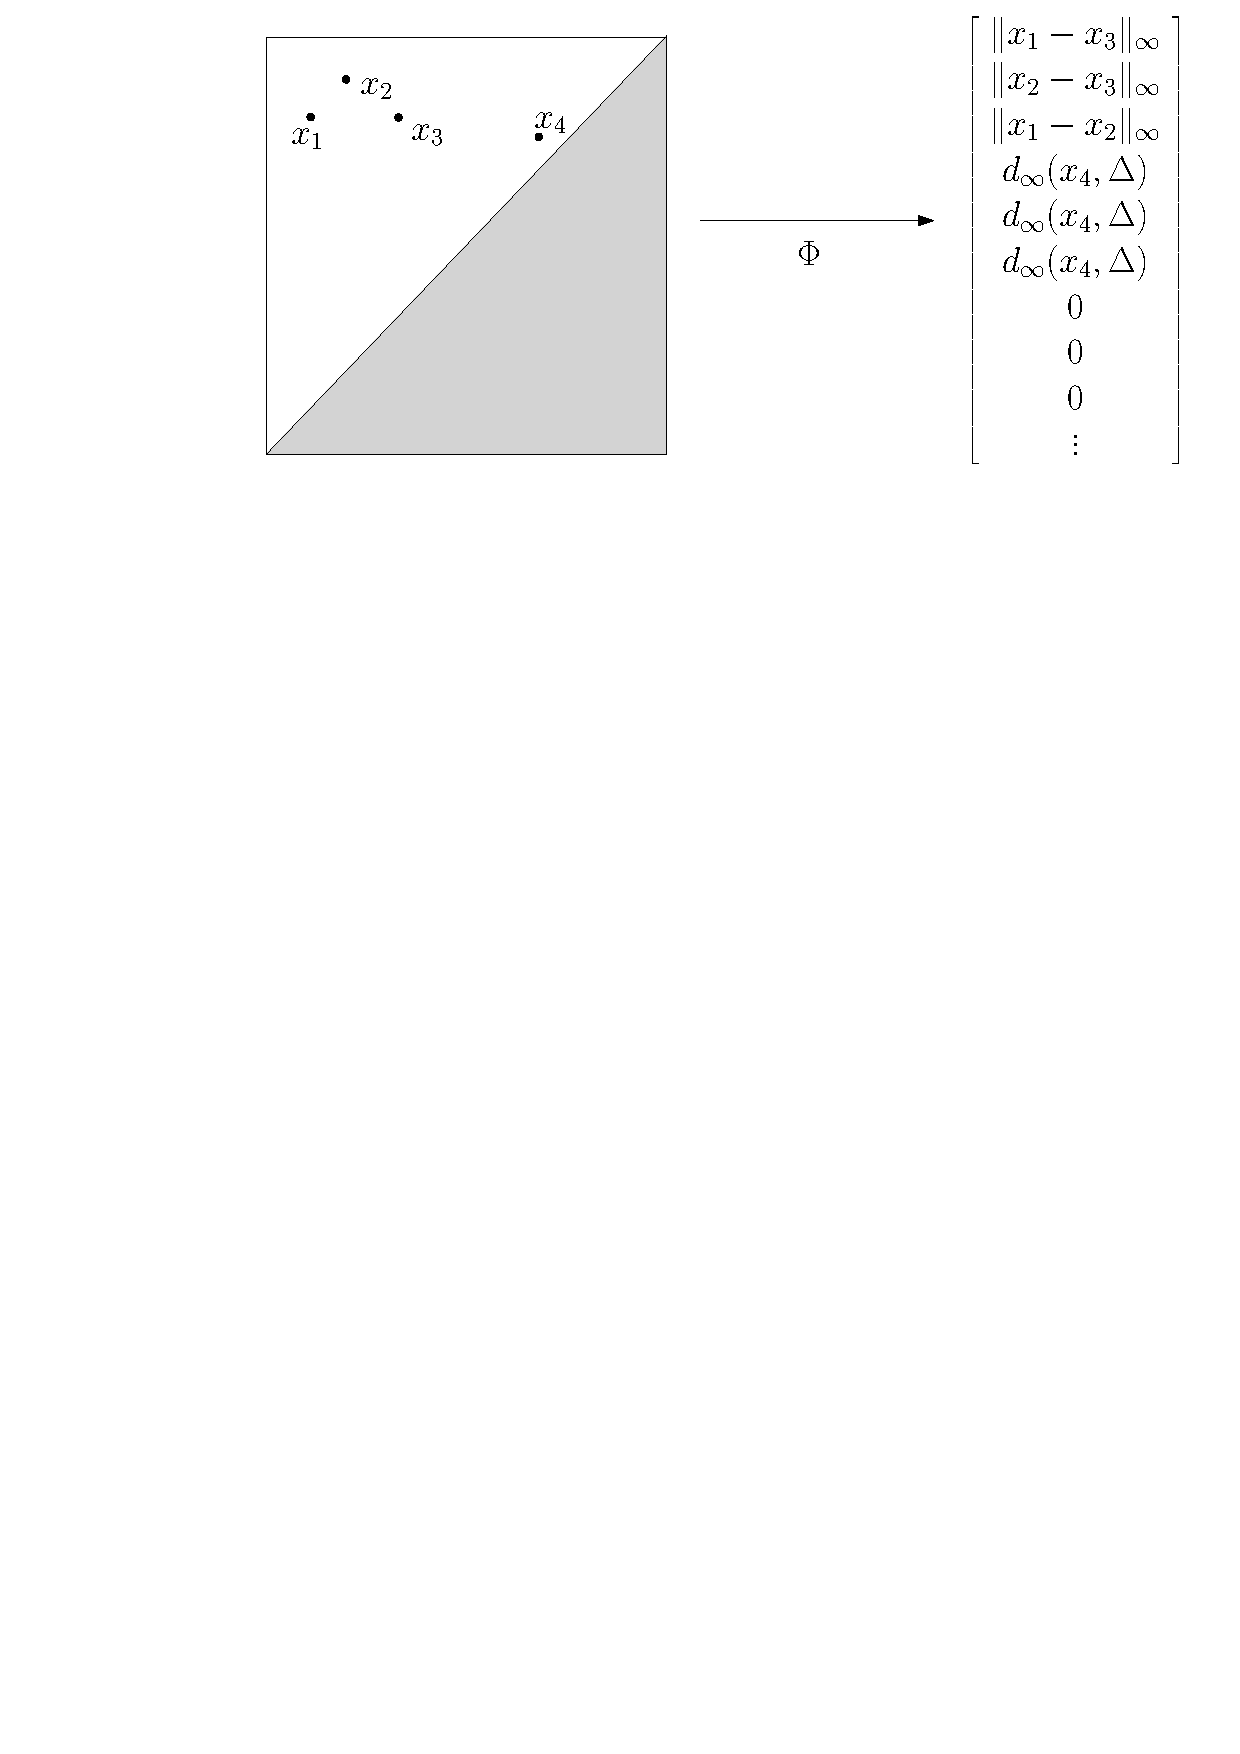
\includegraphics[width = 9cm]{figures/Mapping} 
\caption{\label{fig:Mapping}
Mapping of a persistence diagram to a sequence with finite support. %vector. %, where $d_{\Delta}(\cdot)$ denotes the distance to the diagonal $\Delta$.\vspace{-3mm}
} 
\end{center} 
\end{figure}

\paragraph*{Distances to the diagonal.} 
Another solution is to keep only the sorted distances to the diagonal.
Indeed, this also leads to a stable vectorization that has a significant meaning
since points in persistence diagrams represent topological features---see 
Section~\ref{sec:dictionary} and~\ref{sec:VectorExpe}. 
%On the contrary, pairwise terms in the distance matrix cannot be easily related to intuitive 
%geometric quantities in the data space. 
However, this vector alone lacks discriminative power 
as shown in Figure~\ref{fig:diagpts}. Hence, we concatenate the two vectors in practice.
%
\begin{figure}[h] 
\begin{center} 
%\includegraphics[width = 5cm]{figures/CEBar}
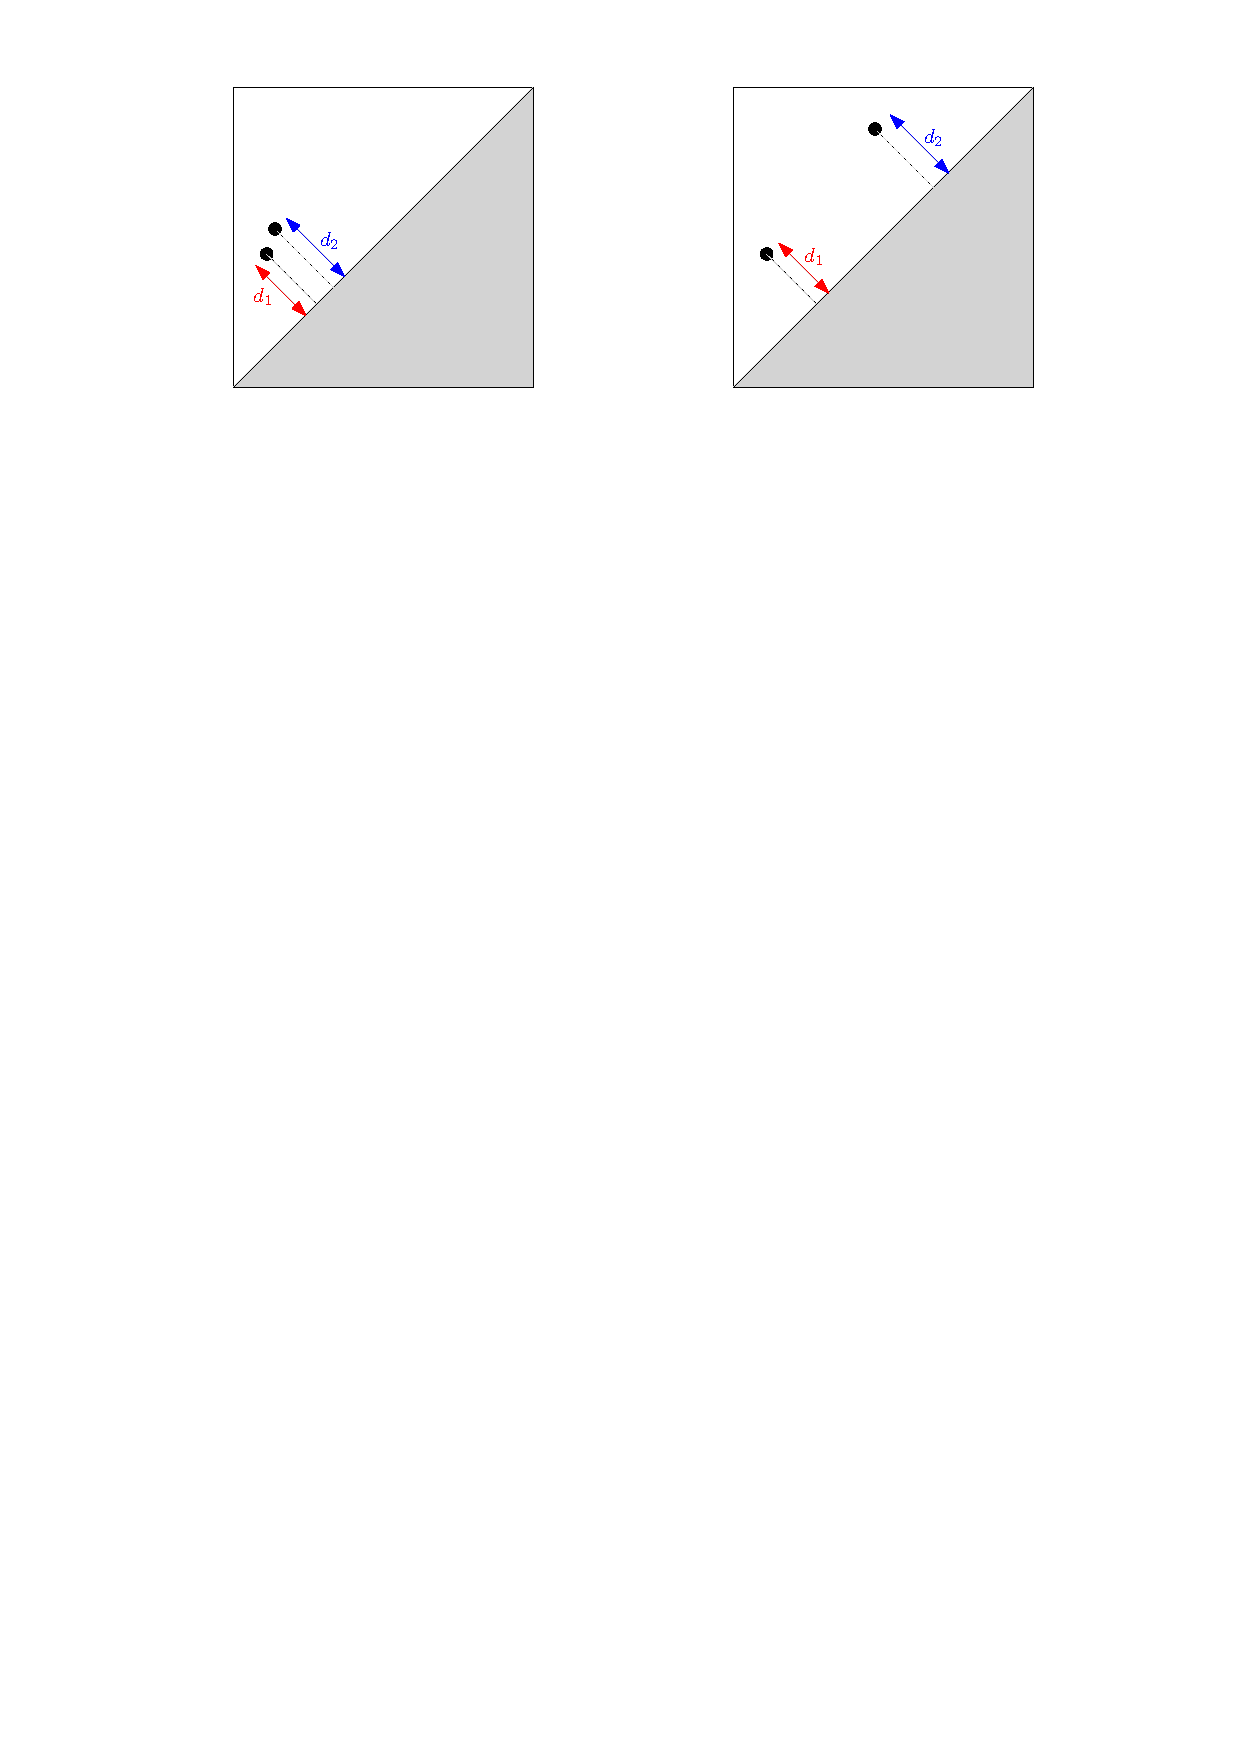
\includegraphics[width = 9cm]{figures/CounterExampleBarPD}
\caption[Distances to diagonal]{\label{fig:diagpts}
%We consider two source points on a synthetic example and their corresponding PDs.
Clearly, keeping only the sorted distances to the diagonal would not
discriminate the two persistence diagrams whereas looking at the distribution
of the distances would allow to successfully distinguish them.} 
\end{center} 
\end{figure}



\paragraph*{Truncation.}
In practice, we want to deal with finite-dimensional vectors of prescribed lengths, so we have to truncate the sequences. 
Since the size of the support of $\Phi(\dg)$ can be quadratic in the number of points in $\dg$, we often
%thus quadratic in the number of points in the shape in 
%the worst practical case of triangle mesh inputs. %We can then try to find ways to reduce the dimension without losing too much information. 
get rid of the last nonzero values, which are also the lowest ones. Note that this is equivalent to getting rid of 
pairwise terms which include either a point very close to the diagonal
or two points which are very close to each other. Thus, by truncation, 
we either get rid of topological noise or get rid of too small distances. In the second case, it does not mean that we do not consider anymore 
the two points as only their mutual distance is removed while their distances to the other points are kept. In practice, we 
truncate the sequences according to some estimated upper bound on the number of relevant topological features in the dataset---see
Section~\ref{sec:VectorExpe} for instance. 

\subsection{Stability of the topological vectors.}\label{sec:StabVect}

In this section, we prove the following stability result:

\begin{thm}
\label{sign}
%Let $(\X,d_\X)$ and $(\Y,d_\Y)$ be two metric spaces. Let $x\in\X$ and $y\in\Y$.
Let $\dg_1,\dg_2\in\SpfD$ be two finite persistence diagrams. %and $\Phi(\dg_1)$ and $V_y$ be their associated topological signatures. 
Let $N_1=\card(\dg_1)>0$, $N_2=\card(\dg_2)>0$ and $N=\max\{N_1,N_2\}$. Let $D=\frac{N(N-1)}{2}$.
Then:
$$C(N)\|\Phi(\dg_1)-\Phi(\dg_2)\|_2\leq\|\Phi(\dg_1)-\Phi(\dg_2)\|_\infty\leq 2\distb(\dg_1,\dg_2),$$
where $C(N)=D^{-\frac 12}$ and $\Phi(\dg_1),\Phi(\dg_2)\in\R^D$.
\end{thm}

\begin{proof}
Let $\e=\distb(\dg_1,\dg_2)$.
As the problem is symmetric in $\dg_1$ and $\dg_2$, 
assume without loss of generality that $N_1<N_2$. 
We consider one of the matchings $\gamma^*$ 
realizing the bottleneck distance between $\dg_1$ and $\dg_2$---such matchings exist since
$N_1,N_2<+\infty$. 
We also call $N_{1,\gamma}$ and $N_{1,\Diag}$ the number of points of $\dg_1$ 
which are mapped by $\gamma^*$ to an element 
of $\dg_2$ and to the diagonal respectively. We have $N_{1,\gamma}+N_{1,\Diag}=N_1$. 
Moreover, $N_{1,\gamma}$ points of $\dg_2$ are mapped to points of $\dg_1$,
$N_{1,\Diag}$ points are mapped to the diagonal, and the $N_2-N_1$ other points of $\dg_2$ 
are also mapped to the diagonal. 
We introduce a bijective mapping 
$\psi:\dg_1\rightarrow\dg_2$ which coincides with $\gamma^*$ 
on the $N_{1,\gamma}$ points of $\dg_1$ which are not mapped to the diagonal  
and which arbitrarily associates the remaining $N_{1,\Diag}$ elements of 
$\dg_1$ to  $N_{1,\Diag}$ remaining  points of $\dg_2$. 
%- here the points associated by $\psi$ were initially mapped to the diagonal by the bottleneck matching. \\

Let $V_1=\Phi(\dg_1)$ and $V_2=\Phi(\dg_2)$.
By definition, we have 
%$$V_1=\left[\ \min\ \{\|p_i-p_j\|_\infty,d_\infty(p_i,\Diag),d_\infty(p_j,\Diag)\}\ \right]_{1\leq i,j\leq N_1}$$
$V_1[i]\geq V_1[i+1],\ \forall 1\leq i \leq N_1(N_1-1)/2$ and $V_1[i]=0$, $\forall i>N_1(N_1-1)/2$,
where $V_1[i]$ denotes the $i$th coordinate of $V_1$.
Now, let $\hat{V}_2$ be the sorted vector of all
%$$\hat{V}_2=[\ 
$\min\ \{\|\psi(p_i)-\psi(p_j)\|_\infty,d_\infty(\psi(p_i),\Diag),d_\infty(\psi(p_j),\Diag)\}$,
where $1\leq i,j\leq N_1$.
We also add the remaining pairwise terms of $\dg_2$ in $\hat{V}_2$ 
%and we also fill $V_1$ with null values until its length is $N_2(N_2-1)/2$
so that $\hat V_2$ has dimension $N_2(N_2-1)/2$. \\

We now show that $\|V_1-\hat{V}_2\|_\infty\leq 2\e$.
Fix a coordinate $i$. Either $i>N_1(N_1-1)/2$, and then
$V_1[i]=0$ and $\hat{V}_2[i]=\min\{\|y_{i,1}-y_{i,2}\|_\infty,d_\infty(y_{i,1},\Diag),d_\infty(y_{i,2},\Delta)\}$, 
for some $y_{i,1},y_{i,2}\in\dg_2$, or  $i\leq N_1(N_1-1)/2$, and then 
$V_1[i]=\min\{\|x_{i,1}-x_{i,2}\|_\infty,d_\infty(x_{i,1},\Diag),d_\infty(x_{i,2},\Diag)\}$, 
and $\hat{V}_2[i]=\min\{\|\psi(x_{i,1})-\psi(x_{i,2})\|_\infty,d_\infty(\psi(x_{i,1}),\Diag),d_\infty(\psi(x_{i,2}),\Delta)\}$,
for some $x_{i,1},x_{i,2}\in\dg_1$. 
We have three different cases to treat here:
\begin{itemize}
\item (a) $i\leq \frac{N_1(N_1-1)}{2}$ and the two pairs of points are matched by $\gamma^*$,

\item (b) $i\leq \frac{N_1(N_1-1)}{2}$ and at least one point of each pair is matched to $\Delta$,

\item (c) $i>\frac{N_1(N_1-1)}{2}$, and then $V_1[i]=0$.
\end{itemize}

Case (c). In this case, at least one of the points of the pairwise term in $\hat{V}_2[i]$, 
say $y_{i,1}$, is matched to the diagonal. Thus, we have
$$|V_1[i]-\hat{V}_2[i]|=|\hat{V}_2[i]|\leq |d_\infty(y_{i,1},\Diag)|\leq\e\leq 2\e.$$

Case (b). In this case, at least one point of the pairwise term in $V_1[i]$, 
say $x_{i,1}$, and one of the pairwise term in $\hat{V}_2[i]$, 
say $y_{i,1}$, are mapped to the diagonal, the other two terms
being either mapped together or to the diagonal. Then
$$|V_1[i]-\hat{V}_2[i]|\leq |d_\infty(x_{i,1},\Diag)|+|d_\infty(y_{i,1},\Diag)|\leq 2\e.$$

Case (a). In this case, we have 
$\gamma^*(x_{i,1})=y_{i,1}$ and $\gamma^*(x_{i,2})=y_{i,2}$. 
Three different subcases come out:
 
\begin{itemize}
\item (i) The minimum is in both cases the distance between the points. Then we have 
$$|V_1[i]-\hat{V}_2[i]|=|\|x_{i,1}-x_{i,2}\|_\infty-\|y_{i,1}-y_{i,2}\|_\infty|\leq 2\e.$$

\item (ii) The minimum is in both cases the distance of a point to the diagonal. 
Then either $$|V_1[i]-\hat{V}_2[i]|=|d_\infty(x_{i,1},\Diag)-d_\infty(y_{i,1},\Diag)|,$$
in which case the bound is immediate as the points are mapped by $\gamma^*$,
or $$|V_1[i]-\hat{V}_2[i]|=|d_\infty(x_{i,1},\Diag)-d_\infty(y_{i,2},\Diag)|,$$
in which case we have the following inequalities:
\begin{itemize}
\item $\eta_x=d_\infty(x_{i,2},\Diag)-d_\infty(x_{i,1},\Diag)\geq 0$,
\item $\eta_y=d_\infty(y_{i,1},\Diag)-d_\infty(y_{i,2},\Diag)\geq 0$,
\item $d_\infty(y_{i,1},\Diag)=d_\infty(x_{i,1},\Diag)+\alpha_1$ with $|\alpha_1|\leq\e$ and
\item $d_\infty(y_{i,2},\Diag)=d_\infty(x_{i,2},\Diag)+\alpha_2$ with $|\alpha_2|\leq\e.$
\end{itemize}

Thus $\e\geq\alpha_1=\eta_x+\eta_y+\alpha_2\geq\alpha_2+\eta_x\geq-\e+\eta_x\geq-\e$ and 
$$|V_1[i]-\hat{V}_2[i]|=|d_\infty(x_{i,1},\Diag)-d_\infty(y_{i,2},\Diag)|=|\eta_x+\alpha_2|\leq\e\leq 2\e.$$

\item (iii) The minimum is the distance of a point to the diagonal for one term 
and the distance between the points for the other, say 
$$\|x_{i,1}-x_{i,2}\|_\infty\leq \min\{d_\infty(x_{i,1},\Diag),d_\infty(x_{i,2},\Diag)\}$$
$$d_\infty(y_{i,1},\Diag)\leq \min\{\|y_{i,1}-y_{i,2}\|_\infty,d_\infty(y_{i,2},\Diag)\}$$ 
Then $|V_1[i]-\hat{V}_2[i]|=|\|x_{i,1}-x_{i,2}\|_\infty-d_\infty(y_{i,1},\Diag)|$. 
As $d_\infty(y_{i,1},\Diag)\geq d_\infty(x_{i,1},\Diag)-\e$, we have 
$$\|x_{i,1}-x_{i,2}\|_\infty-d_\infty(y_{i,1},\Diag)\leq\e+(\|x_{i,1}-x_{i,2}\|_\infty-d_\infty(x_{i,1},\Diag))\leq\e\leq 2\e$$
We also have 
$$d_\infty(y_{i,1},\Diag)\leq \|y_{i,1}-y_{i,2}\|_\infty\leq \|x_{i,1}-x_{i,2}\|_\infty+2\e,$$
and thus
$$|V_1[i]-\hat{V}_2[i]|\leq 2\e.$$ 
\end{itemize}

Finally, $\|V_1-\hat{V}_2\|_\infty\leq 2\e$. 
Now we prove and use the following lemma to conclude:

\begin{lem}\label{interm}
Let $D\in\N$ and $U,\hat V\in\R^D$. 
Assume that $U$ is {\em non-increasing}: $\forall i,j\in \{1\ ...\ n-1\}$, $i\leq j \Rightarrow U[i]\geq U[j]$.
Let $V\in\R^D$ be the image of $\hat V$ by a coordinate permutation $\sigma$ which 
makes it non-increasing: $\forall i,j\in \{1,\cdots,n-1\}$, $V[\sigma(i)]=\hat V[i]$ and 
$i\leq j \Rightarrow V[i]\geq V[i+1]$. Then:
$$\|U-V\|_\infty\leq\|U-\hat V\|_\infty.$$ 
\end{lem}

\begin{proof}
Let $\alpha=\|U-\hat V\|_\infty$.
%Since $\|U-V\|_{\infty}=\alpha$, we can always bound $v_i:=V[i]$ between 
%$U[i]-\alpha$ and $U[i]+\alpha$. \\ 
Let $i\in\{1,\cdots,n\}$ and $\hat v_i=\hat V[i]= U[i] + x_i$, 
where $-\alpha\leq x_i\leq\alpha$. 
Let $\sigma$ be the coordinate permutation between $V$ and $\hat V$, i.e. $\hat v_i=V[\sigma(i)]$.
%When computing the infinite norm of $U-\tilde{V}$, we have to estimate the position $\sigma(i)$ of $v_i$ in $\tilde{V}$, i.e.
%the integer $l_i$ such that $\tilde{V}[l_i]=v_i$.
Let $m(i),M(i)\in\N$ be defined as:
$$M(i)=\min\ \{t\,:\,U[t]+\alpha<\hat v_i\}$$
(or $M(i)=n+1$ if the set is empty) and
$$m(i)=\max\ \{t\,:\,U[t]-\alpha> \hat v_i\}$$
(or $m(i)=0$ if the set is empty). Note that $m(i)<i<M(i)$ by definition.
Since $t\leq m(i)\Rightarrow \hat V[t]>\hat V[i]$ and  $t\geq M(i)\Rightarrow \hat V[t]<\hat V[i]$,
there are at least $m(i)$ terms in $\hat V$ that are strictly larger than $\hat v_i$, and $D-M(i)+1$
that are strictly smaller. Since $V$ is non-increasing, it follows that:
$$m(i)+1\leq \sigma(i) \leq M(i)-1.$$

Using the definition of $m(i)$, the fact that $U$ is non-increasing and the equality $\hat v_i=U[i]+x_i$, we have 
%$U[m(i)+1]-U[i]\geq U[\sigma(i)]-U[i]$. Moreover, by definition: $U[m(i)+1]\leq v_i+\alpha$, and thus 
$U[\sigma(i)]-U[i]\leq U[m(i)+1]-U[i]\leq\alpha+x_i$.
Since $U[\sigma(i)]-V[\sigma(i)]=U[\sigma(i)]-\hat V[i]=U[\sigma(i)]-U[i]-x_i$, it follows that
$$U[\sigma(i)]-V[\sigma(i)]\leq\alpha.$$

Similarly, we have $U[\sigma(i)]-U[i]\geq U[M(i)-1]-U[i]\geq x_i-\alpha$, and thus
$$U[\sigma(i)]-V[\sigma(i)]\geq-\alpha.$$

Finally, we have $|U[\sigma(i)]-V[\sigma(i)]|\leq\alpha.$
This inequality being true for all $i$, it is also true for the vectors in the infinite norm and the proof is complete.
\end{proof}

We can finally conclude : $\|V_1-V_2\|_\infty\leq \|V_1-\hat V_2\|_\infty\leq 2\e$.
\end{proof}


\paragraph*{Analysis of the stability bound.}
The dependence on $N$ can lead to very small constants $C(N)$ in the worst case, which is
not desireable as in practice.
%, the vectors have sizes varying between 50 and 500.
However, two remarks are worth considering at this point.
Firstly, this constant disappears using the infinity norm, which is useful when using e.g. kNN classifiers.
Secondly, this constant can be reduced by truncating the vectors, as stability is preserved whatever the 
number of components kept. In return, the vectors are less discriminative, so a trade-off has to be made in practice.
%, but we show this loss 
%is acceptable in our application. 
%We recall that truncation is an important feature for two reasons: first, because by reducing the dimension of the
%vectors we actually reduce the constant $C(N)$ in the previous
%equation; second, because entries of the vectors that include points
%close to the diagonal may not be significant and descriptive
%at all, so we can get rid of them without compromising the stability.

\subsection{Application to 3D shape processing}
\label{sec:VectorExpe}

In this section, we detail an application of persistence diagrams and corresponding
 topological vectors  in 3D shape processing, 
in which descriptors are required to be Euclidean vectors.
More precisely, we use persistence diagrams as {\em point descriptors}
for {\em 3D shape segmentation}.  

\paragraph*{Notation.}
We use {\em shape} as a shorthand for a compact smooth surface in $\R^3$.

\paragraph*{Persistence diagrams as point descriptors.}
In order to provide a multiscale description of the structure of a shape $X$ from the 
point of view of a single point $x\in X$, 
we consider the filtration induced by growing a geodesic ball
centered at $x$, with radius $r$ going from $0$ to $+\infty$, i.e. the filtration induced by 
the sublevel sets of the distance function $f_x(\cdot)=d(x,\cdot)$---see
Figures~\ref{fig:geodesic-ball1} and~\ref{fig:geodesic-ball2}. We then encode the evolution of the ball's homology
in the corresponding persistence diagram.
%including its connected components (dimension 0), holes (dimension 1), and enclosed voids (dimension 2). 
Since we are dealing with surfaces, the 0-dimensional persistent homology is always trivial, whereas the 
2-dimensional persistent homology has
limited information (there is just one enclosed void, namely the surface itself).
%as mentioned in Section~\ref{sec:Duality}. 
%Therefore, we can restrict ourselves to the first persistence diagram only. 
Hence, in practice, we compute the 1-dimensional persistence diagram and we add an extra point
representing the unique 2-dimensional homological feature of the shape.
%an extra point to its corresponding PD,
%which has a null abscissa and an infinite ordinate equal to the radius for which the geodesic ball
This extra point has an infinite ordinate and an abscissa equal to
the eccentricity of the source point.
%the radius for which the geodesic ball
%centered on the source point is the shape itself.
%As this extra point coordinates correspond to 0D and 2D persistence,
%Adding it does not affect Theorem~\ref{sign}, which is stated in any dimension.
In particular, this allows distance-to-diagonal terms to naturally appear
in the topological vector---see Definition~\ref{def:MappingSeq}. 
Finally, we also add  the distance to the diagonal 
of this extra point in the topological vector since 
%this quantity is related to the eccentricity and, 
this does not affect its stability.

%The number of such holes, given a specific radius, is exactly 
%the so-called {\em Betti number}~$\beta_1$. Intuitively, a hole is either 
%a boundary component of the ball, or a handle or tunnel (like in the torus) included in it. 
%Another interpretation is to consider the shape as a geographic
%landscape. Then every boundary hole that appears during the
%growing process is associated to a specific bump, or mountain, of the landscape.
%Thus, a good idea to start with would be the computation of $\beta_1$,
%or even the Euler characteristic $\chi$ of the geodesic ball, for
%every radius. This would give us an integer-valued function defined
%over the radii for every center point $x$.  However, it turns out that
%such functions, in addition to being difficult to store, are not
%stable as a slight variation in the position of the center point $x$,
%or a slight perturbation of the shape, would induce big differences in
%infinity norm between them. Even if we turn these integer-valued
%functions into real-valued vectors by storing the radii for which
%\beta_1$ changes, they are actually still not stable as jumps can
%still occur.


%
\begin{figure*}[t!] 
\begin{center} 
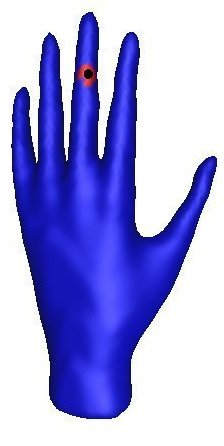
\includegraphics[height = 3.3cm]{figures/dist1} 
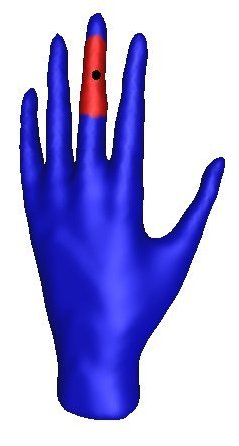
\includegraphics[height = 3.3cm]{figures/dist2} 
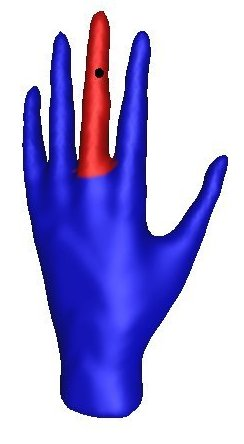
\includegraphics[height = 3.3cm]{figures/dist3}
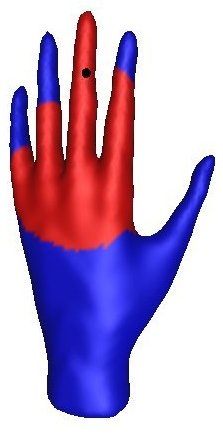
\includegraphics[height = 3.3cm]{figures/dist4} 
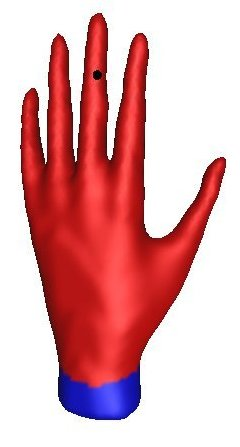
\includegraphics[height = 3.3cm]{figures/dist5} 
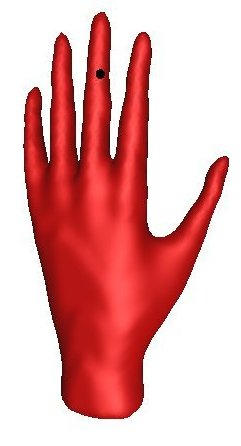
\includegraphics[height = 3.3cm]{figures/dist6}
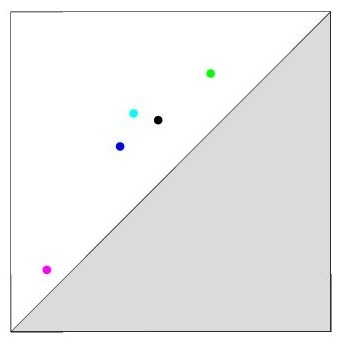
\includegraphics[height = 3.5cm]{figures/PD3}  
\caption[Geodesic balls]{\label{fig:geodesic-ball1} Geodesic balls centered at the
  black point are displayed in red. The persistence diagram
  corresponding to this family is shown in the far right. Note that each
  point can be easily associated with a shape part. The pink, blue,
  light blue, black and green points correspond to the middle, index,
  ring, pinky and thumb respectively. As the center point is close to
  the tip of the middle finger, one can see that its point in the persistence diagram
  is much closer to the diagonal than the other fingers. Note that
  for this shape, there are no essential holes.}
\end{center}
\end{figure*}

%
\begin{figure*}[t!] 
\begin{center} 
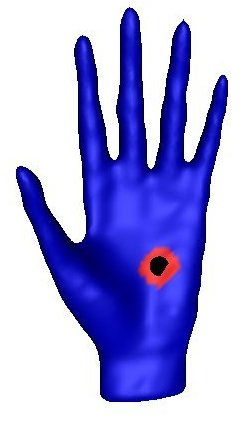
\includegraphics[height = 3.3cm]{figures/dist7} 
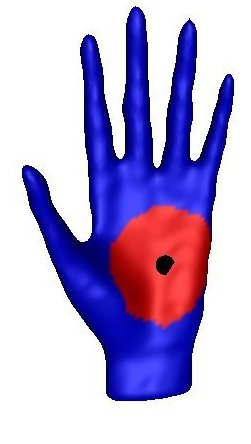
\includegraphics[height = 3.3cm]{figures/dist8} 
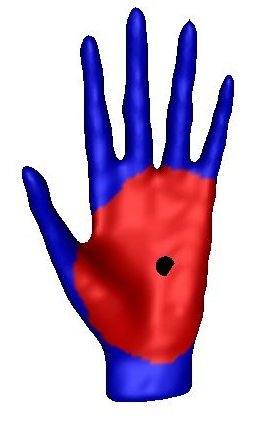
\includegraphics[height = 3.3cm]{figures/dist9}
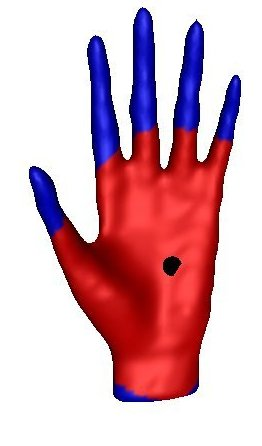
\includegraphics[height = 3.3cm]{figures/dist10} 
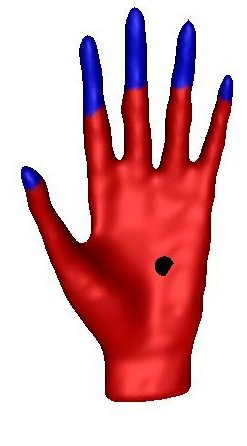
\includegraphics[height = 3.3cm]{figures/dist11} 
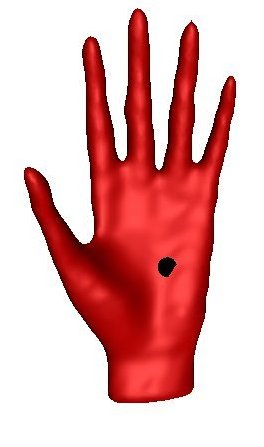
\includegraphics[height = 3.3cm]{figures/dist12}
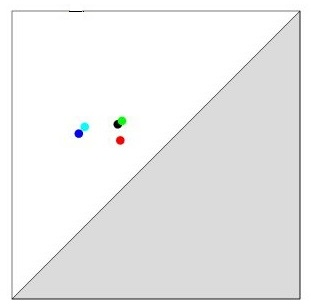
\includegraphics[height = 3.5cm]{figures/PD2}  
\caption[Geodesic balls]{\label{fig:geodesic-ball2} Same process as
  Figure~\ref{fig:geodesic-ball1} but with a different center
  point. Note the difference in the persistence diagram (far
  right). The colors in the diagram correspond to the same parts of
  the hand as in Figure~\ref{fig:geodesic-ball1}. There is, however a
  new point in red, which corresponds to the hand base (palm), which
  was not present in the persistence diagram of the previous shape.}
\end{center} 
\end{figure*}




%This is why our tracking is a little bit different and adds more
%information.  
%\paragraph*{Interpretation of the persistence diagram.} 
%We informally recall that computing 1-dimensional persistent homology in this context 
%can be performed by computing the values of the radius
%$r$ for which the number of holes in the ball changes, and by pairing
%the values corresponding to the same hole. More precisely, to each
%hole are associated two values: the one at which it appears, called
%the {\em birth value}, and the one at which it gets filled in, called the {\em death value}.
%or merged into another one, called the {\em death value}. To decide which
%%one of the two holes dies after a merge, we use the so-called {\em
%%elder rule}, which states that the hole that disappears is the
%%younger one, meaning the one that appeared for the larger value of $r$.  
%When a hole does not eventually get filled in, it is called an {\em essential hole} because it is a
%topological feature of the entire shape $X$, and as such its death
%value is set to $+\infty$. 
%Given a base point $x$, we can therefore store the 1-dimensional topological
%information associated to the growing family of geodesic balls
%$\{B(x,r)\,:\,r\in\R_+\}$ in the first persistence 
%diagram. In this diagram, every hole has two coordinates, the
%abscissa being the birth value and the ordinate being the death
%value. This diagram is thus a multi-set of points, that are all above the diagonal
%$\Diag$ in the extended plane $\overline{\R}^2$. Note
%that we need to give multiplicities to the points as different holes can
%appear and disappear at the same radii. 

%We refer the reader to Chapter~\ref{chap:backgroundHomologyPersistence} for more details
%on persistent homology.

\paragraph*{Distance to the diagonal.} We also recall that the distance to the diagonal has a specific meaning. Indeed,
if a point is very close to or is on the diagonal, it means that the corresponding hole was filled in quickly after
being born in the growing process. In the case of 3D shape processing, this can be interpreted as
a bump of small topographic prominence for instance, which can be considered as topological noise. The vertical
distance of a point to the diagonal is exactly the prominence of the corresponding bump.
On the contrary, the more salient a bump, the longer its prominence and thus the further away from the diagonal its point.


\paragraph*{Example.}
We illustrate two such trackings for two different black center points in
Figures~\ref{fig:geodesic-ball1} and ~\ref{fig:geodesic-ball2}.  The growing process is shown from
left to right with geodesic balls colored in red. If we consider Figure~\ref{fig:geodesic-ball1}, we
can see that in the first (left-most) image, the geodesic ball has no non-contractible cycles
(holes) as it is simply connected.  In the second image, the geodesic ball contains one inessential
hole (at the tip of the middle finger). In the third one, there are no non-contractible holes again
as the previous one is now filled in.  In the fourth image, there are three inessential holes (the
three other fingers). In the fifth one, there are no holes (notice that the thumb created a
hole that was born and filled in between the fourth and fifth images).  In the last image, the
geodesic ball contains the entire shape, which has spherical topology and, as such, contains no
essential holes. Therefore, the persistence diagram contains no points at infinity. Note that since
the black base point is close to the tip of the middle finger, one of the points in the
persistence diagram is both born and dead significantly earlier than the other ones.
%As the center point is close to the tip of the middle finger, one can see that
%its point in the PD is much closer to the diagonal than the other fingers.

%As illustrated in Figures ~\ref{fig:geodesic-ball1} and ~\ref{fig:geodesic-ball2}, persistence
%diagrams characterize the topology of the shape centered around a point at multiple scales. 

%\paragraph*{Properties.}
%Persistence diagrams are intrinsic, as they only use geodesic distances on the shape (as opposed to other descriptors which
%use the ambient Euclidean metric in $\R^3$) and as such are invariant to both intrinsic
%and extrinsic isometries. Moreover, they are also stable with respect to small
%non-isometric perturbations of the shapes---see Section~\ref{sec:Stability}.  In particular, the
%diagrams remain close to each other for slight variations of the center point or of the shape.

\paragraph*{Truncation level.}
%To sum up, for every point in the shape, we compute its persistence diagram and then we derive a descriptor by taking
%a truncation of the sorted sequence given by $\Phi$---see Definition~\ref{def:MappingSeq}. 
%Thus, each shape leads to a collection of vectors
%of possibly different sizes.  
The truncation level (or equivalently the dimension of the topological vectors) is driven by the prominent holes of each category
(for instance this number would be 5 for a human shape---two legs, two arms and the head---thus we would 
only keep around 5(5-1)/2=10 components in the vectors).
In order to make the vectors independent of the scale, we
consider the diagrams in log-scale (meaning that we apply the function $\log(1+\cdot)$ 
on every birth and death value). 
%during the computation of the signatures. 
%As we are storing only the
%1D topological information (holes), we refer to these
%diagrams as 1D persistence diagrams.


\paragraph*{MDS and kNN.} As an illustration, Figure~\ref{fig:MDS} shows the
topological vectors of all the points of a specific shape, plotted as points in
$\R^3$ after a MultiDimensional Scaling (or MDS) on their
distance matrix. The color of each vector is given by a
ground truth segmentation provided with the input data set. Two
remarks are in order at this stage: first, note that there is some
continuity between vectors with identical labels, which suggests that the
topological vectors vary continuously along the shape; second, and consequently, there is no natural grouping of the
vectors into clusters, so unsupervised segmentation using
traditional clustering algorithms such as k-means is likely to be
ineffective. These observations suggest rather to use supervised
learning algorithms in segmentation applications.
We also show how such a kNN segmentation 
allows to achieve reasonable performance in Figure~\ref{fig:kNN}, 
even though the use of more elaborate algorithms like SVM leads to better results.
%It is interesting as such a simple task would be impossible with , as explained in Section~\ref{sec:Vectors}.


\begin{figure}[h] 
\centering 
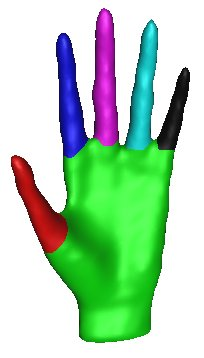
\includegraphics[width = 3cm] {figures/hand_mds}
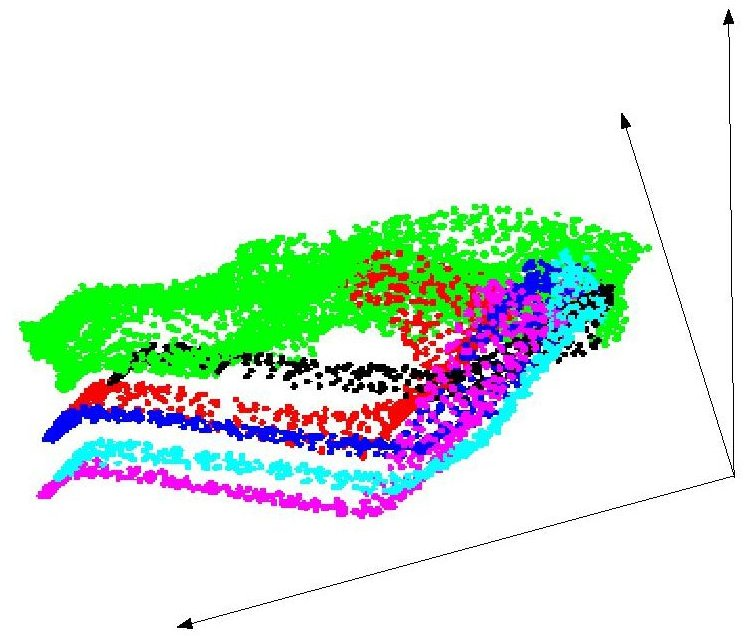
\includegraphics[width = 7.5cm] {figures/mdshand3}
\caption[MDS on topological vectors]{\label{fig:MDS}
Example of MDS. One can easily observe the continuity between vectors of different labels.
The color of each point refers to the same label as the colors displayed on the hand shape.} 
\end{figure}

\begin{figure}[t!] 
\begin{center} 
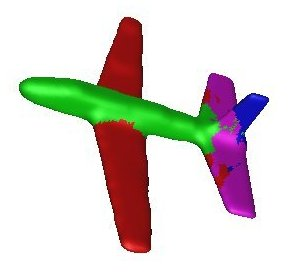
\includegraphics[height = 4cm]{figures/kNN1} 
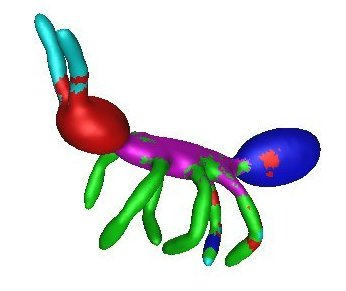
\includegraphics[height = 4cm]{figures/kNN2}
\caption[kNN on topological vectors]{\label{fig:kNN} We compute the most common
	label for each face in a set of 100 nearest neighbors computed from
	a training set. No smoothing is applied but the segmentations on this pair of shapes are still reasonable
	(around 80 percent accuracy). However, this accuracy can decrease to 60 percent
	in other categories, thus we need a more elaborate algorithm for segmentation.}
\end{center}
\end{figure}




%\paragraph*{Signature for metric spaces.} Finally, note that the definition of our signature 
%holds more generally for compact metric spaces, so our signature can
%be used on a much wider class of spaces than 3D shapes, and in
%potentially many applications. In particular, our
%mapping of persistence diagrams to vectors could be used on the global
%signatures of~\cite{Chazal09c}, or even for characterizing objects of
%different nature, like images as in~\cite{Li14}. Moreover, note that our family of growing balls
%can be seen as the sublevel sets of a distance function to the base point. Indeed, one could also
%compute PDs with sublevel sets of other functions, leading to a high modularity of our signature.
%In Section~\ref{sec:PD-computation}, we give the algorithm to compute persistence diagrams
%from the sublevel sets of an arbitrary function.



\paragraph*{Stability.}
The main advantage of considering 
the persistence diagrams is that they enjoy stability properties, meaning that
the difference between two diagrams cannot be too large if the
they are computed from nearby points or on nearby shapes.  
This stability is a key feature in applications. It is stated formally in~\cite{Carriere15b}.
%Recall that the construction of our signature proceeds in two
%stages. Below we present the stability theorems of each stage
%independently.  We begin by stating the stability of the constructed
%PDs, which requires to introduce their natural metric called the
%\textit{bottleneck distance} $d_b^\infty$. 
%Stability is expressed in
%terms of perturbations of the center point and of the overall shape,
%as measured by metric distortions of correspondences. 

%We then state
%the stability of the derived vectors in the Euclidean and
%$\ell^\infty$-norms, in terms of perturbations of the PDs in the
%bottleneck distance. Note that this second stability result holds
%generally, in particular when our mapping from PDs to vectors would be
%applied to the global signatures, such as the ones defined
%in~\cite{chazal2009gromov}.
%The statements given in full generailty and their proofs
%are provided in~\cite{proofs}. Here, we only mention their simplest versions,
%which are sufficient for our purposes.

%\paragraph*{Stability for PDs.} 


%Intuitively, if we perturb two shapes by modifying the metric distortion
%of their correspondences, it will also perturb the locations of the prominent
%bumps, leading to coordinate changes for the points in their corresponding PDs.
%In practice, our inputs are finite metric spaces and come from triangle mesh 
%samplings of the manifolds and an associated graph distance (such as the shortest path along edges).
%As the proof of the theorem does not use the triangulation of the shape, 
%goes through the analysis of PDs derived from finite samplings of the shapes, 
%one can easily extend Theorem~\ref{th:stabilityPD} to these finite metric spaces 
%approximating the shapes in the Gromov-Hausdorff distance~\cite{Burago01}.
%Furthermore, the proof holds more generally 
%for a broad class of functions, of which distance functions are but a small excerpt---then, 
%the general statement involves an extra term depending 
%on the so-called \textit{functional distortion} of spaces,
%and also for smooth compact Riemannian manifolds and persistence diagrams of arbitrary dimensions.
%We refer the interested reader to~\cite{Carriere15b} for formal statements and proofs.
%for the formal statement and proof.

%\paragraph*{Illustration of the stability.}
As an illustration of this stability property, we display components
of topological vectors on shapes in various poses 
%(relatively to the Gromov-Hausdorff distance~\cite{burago2001}) 
in Figure~\ref{fig:preserv}. 
Theorem%~\ref{th:stabilityPD} %and
~\ref{sign}  
ensure that corresponding points have similar vectors. 
%Although it is hard to intuitively guess where large and small values of the components of our signature are located on the shape,
Note that the components of the topological vectors characterize parts of the shape that are difficult to relate to 
the other classical descriptors in the literature---apart from the first component, which roughly corresponds to the eccentricity---see
the second paragraph of this section. 
%Nevertheless, this is not too much of an issue, 
%as our primary goal is to derive a stable and powerful descriptor
%without placing importance on its interpretation.

\begin{figure}[t!] 
\begin{center}
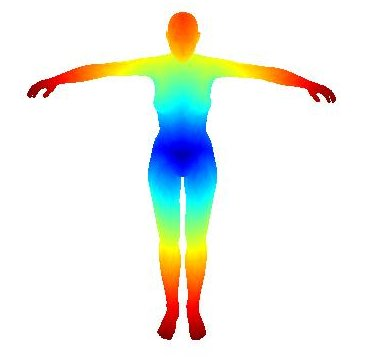
\includegraphics[height = 3.5cm]{figures/stab13}\ \ \ \ 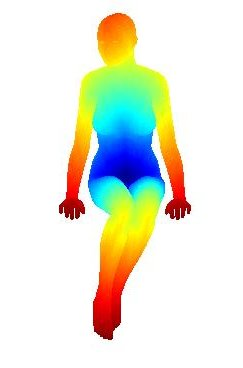
\includegraphics[height = 3.5cm]{figures/stab14}\ \ \ \ 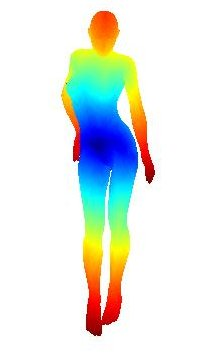
\includegraphics[height = 3.5cm]{figures/stab15}

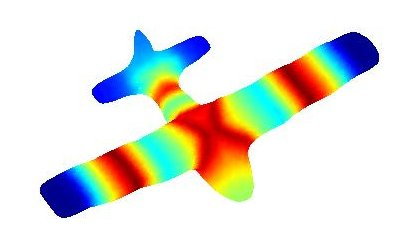
\includegraphics[height = 2.5cm]{figures/stab7}
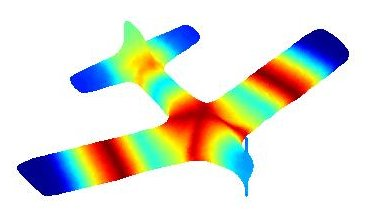
\includegraphics[height = 2.5cm]{figures/stab8}
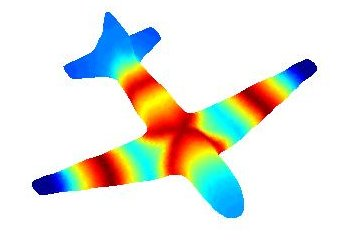
\includegraphics[height = 2.5cm]{figures/stab9}

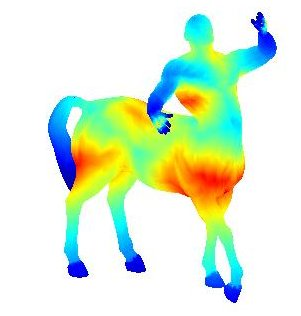
\includegraphics[height = 3cm]{figures/stab10}
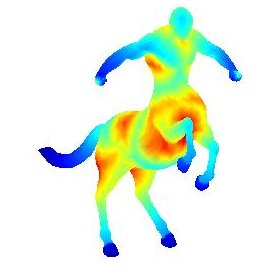
\includegraphics[height = 3cm]{figures/stab11}
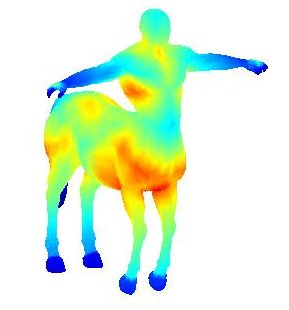
\includegraphics[height = 3cm]{figures/stab12}  
\caption[Stability of topological vectors]{\label{fig:preserv} Topological vectors are computed on
nearly isometric shapes. The first component is shown on the human shape,
the second component is shown on the planes and the third one is shown on the centaurs.
One can see that it respects the 
correspondence due to its stability.}
\end{center}
\end{figure} 






\paragraph*{Computation.}
Unfortunately, 1-dimensional persistence is costly to compute in general. %~\cite{Morozov08}. 
%and persistence diagrams 
%are not naturally amenable to standard learning algorithms as there is no simple way to compare the diagrams
%associated with two different points. This is an important problem as signature comparison is a key
%and recurring step in many shape processing and analysis algorithms. In the rest of the paper, we
%show how both these issues can be addressed. 
%We now show that by using duality theorems, the
%computation of 1-dimensional persistence can be reduced to the zero-dimensional case, which is significantly
%easier to deal with in practice. %(Section~\ref{sec:Duality}). 
%As mentioned earlier, computing the complete 1D persistence of shapes is costly. 
Indeed, if the shape is given by a triangle mesh with $O(m)$ edges and faces, the worst-case running time is
of the order of $O(m^3)$~\cite{Morozov08}. Note that this running time is the same for every
center point.
%In particular, if the input is a point cloud sampling of the shape, the algorithm complexity for 1D-persistence 
%is cubic in the number of points in the worst case. 
To overcome this difficulty in the case of 2D surfaces, we use Theorem~\ref{th:EPsym},
%theorems~\cite{Cohen09,deSilva11}. 
%These theorems establish the
%correspondence between $k$-dimensional persistence, for $k\in\{0,1,2\}$. 
which states
the equivalence between the inessential holes of the family of balls, i.e. points in $\Ord_1(f_x)$ and the inessential connected
components (0-dimensional persistence) of the family of complements of these balls, i.e. points in $\Ord_0(-f_x)$. This means that, within
every geodesic ball, every hole is associated to a connected component of the ball's complement. As
connected components are much easier to track than holes (the complexity of computing 0-dimensional persistence
diagrams is nearly linear), it is preferable to use them instead. Notice that, as we study the
family of complements, the birth values are now bigger than the death ones (as the radius is
decreasing), leading to points under the diagonal. As an illustration,
consider the family of the complements in Figure~\ref{fig:geodesic-ball1} (displayed in blue).
Connected components of the blue sets are related to the holes of the red ones.
%As an illustration, consider the family of the complements in Figure~\ref{fig:geodesic-ball1}
%(displayed in blue).  The evolution is now from right to left.  In the first picture, there are no
%connected components (cc).  In the second one, there is only the essential cc.  In the third one,
%there are three inessential cc and the essential one.  In the fourth one, there is only the
%essential cc again .  In the fifth one, there is one inessential cc and the essential one.  Finally,
%in the last one, there is only the essential cc.  The hand base (in red) is associated to the
%essential cc while all the fingers represent inessential cc and thus inessential holes.
%Thus, PDs computed from 0D-persistence of the ball complements give information on both 1D and 2D-persistence, 
%in the sense that to every point in the PD which is not located at the infinity (thus inessential) is associated an 
%inessential hole and to the point located at the infinity (there is one as our shapes are connected) is associated 
%the cavity at the interior of the shape.
However, note that Theorem~\ref{th:EPsym} for essential holes, i.e. points in $\Ext_1(f_x)$, only associates them with essential
holes of the complements, i.e. points in $\Ext_1(-f_x)$.  
The essential connected components of the family of complements of balls, i.e. points in $\Ext_0(f_x)$,
are associated with the essential enclosed voids (2-dimensional topology) of the family of balls, i.e. points in $\Ext_2(-f_x)$, (see Figure~\ref{fig:dual}).
Thus, we cannot get access to the essential holes (the global loops or handles
on the shape) with 0-dimensional persistence. This means that, although we gain a significant speedup in
computational complexity, we lose some information when using duality, and in particular we do
not track essential holes of 1-dimensional persistence.  

%
\begin{figure*}[t!] 
\begin{center}
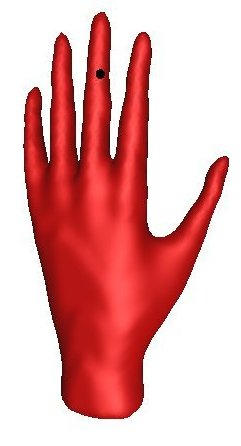
\includegraphics[height = 3cm]{figures/dist6}\hspace{3mm}
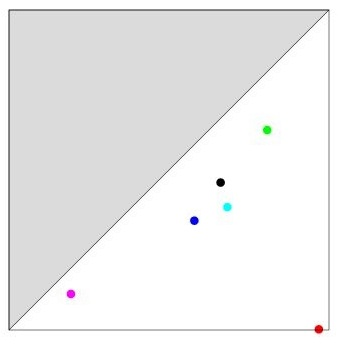
\includegraphics[height = 3.3cm]{figures/PD1} 
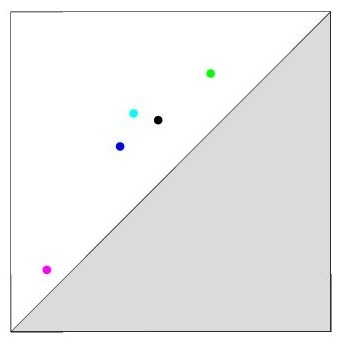
\includegraphics[height = 3.3cm]{figures/PD3} 
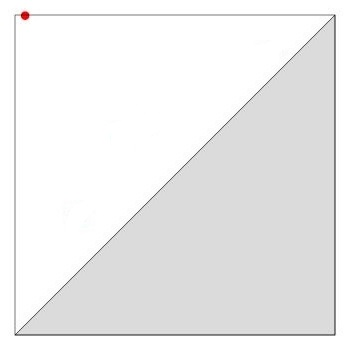
\includegraphics[height = 3.3cm]{figures/PD4}  
\caption[Symmetry]{\label{fig:dual} Left: base point shown in black. Middle: the 0, 1 and 2-dimensional
  persistence diagrams of the family of complements (0-dimensional) and the family of geodesic balls (1-dimensional and
  2-dimensional).  The symmetry theorem establishes the correspondence between the inessential points of the 0-dimensional
  and 1-dimensional persistence diagrams. They also match the essential point of the left-most persistence diagram (in red) with the
  essential point of the right-most persistence diagram. On this example, the 1-dimensional persistence diagram has no essential
  point, but if it had one, we would not be able to capture it in the 0-dimensional persistence diagram.}
\end{center} 
\end{figure*}

\paragraph*{3D shape segmentation.}
%To demonstrate the performance of this descriptor, 
In this paragraph, we use the topological vectors for supervised 3D
shape segmentation and labeling.
We use the Princeton benchmark~\cite{Chen09} for both training and test shapes. This benchmark
contains several different ground truth segmentations for each shape. On each shape that we use in
the training set, we use the same ground truth segmentation as Kalogerakis et
al.~\cite{Kalogerakis10}. 
%(that is the segmentation with lowest average 
%Rand Index to all other segmentations for that shape). 
To show the improvement obtained when using our vector, we first consider the segmentation
produced by using the method with 5 training shapes per category and the subset of
features used in~\cite{Kalogerakis10}. Table \ref{tab:RI} (second column) shows an error percentage (computed with the Rand Index, 
%given as a percentage
which measures the segmentation quality as defined in~\cite{Chen09}, lower is better) obtained without using the topological vectors. 
In the same table (third column, S5+PDs) 
we report the error obtained by using the same
pipeline, but augmented with the topological vectors, which on average has 15-20 dimensions.
We recall---see the paragraph on symmetry---that the topological vectors cannot get access to essential hole (handles).
This explains why the improvement is low in categories for which the segmentation characterizes handles (e.g. Cups).
Other algorithms can be used to compute the full 1-dimensional homology~\cite{Morozov08} but they are more costly.
We also believe that the bad result in the Glasses category is due to the fact that there are no
prominent bumps on the Glasses shapes leading to nearly equal topological vectors almost everywhere that fool
the classifier in the training process.
Apart from that, note that in 18 out of 19 categories, we obtain an often significant improvement in the results. We also compare
these results with the method of~\cite{Kalogerakis10}, which uses 6 and 19 training shapes (S6
and S19, respectively fourth and fifth columns of Table \ref{tab:RI}). Note that in 12 out of 19
categories our results are better than S6 and in 4 out of 19 categories better than S19, even though we
used fewer training shapes, fewer features in each training shape, and no expensive penalty matrix optimization.  
Overall, this table shows that we can get close to the optimal results (where all-but-one shapes are used for training,
leading to a huge amount of running time) with 
less data and features and demonstrate that topological vectors provides complementary information to the
existing descriptors, and can potentially be useful in shape segmentation and labeling scenarios.

\begin{table}[t!]
\begin{center}
\begin{tabular}{|c|c|c|c|c|c|}
  \hline
   & S5 & S5+PDs & S6 & S19\\
  \hline
  Human & 21.3 & \textit{\textbf{11.3}} & 14.3 & 11.9 \\ 
%-10.0
\hline
  Cup & 10.6 & \textit{10.1} & 10.0 & \textbf{9.9} \\
%-0.5
\hline
  Glasses & 21.8 & \textit{25.0} & 14.1 & \textbf{13.7} \\
%+3.2
\hline
  Airplane & 18.7 & \textit{9.3} & 8.0 & \textbf{7.9} \\
%-9.4
\hline
  Ant & 9.7 & \textit{\textbf{1.5}} & 2.3 & 1.9 \\
%-8.2
\hline
  Chair & 15.1 & \textit{7.3} & 6.1 & 5.4 \\
%-7.8
\hline
  Octopus & 5.5 & \textit{3.4} & 2.2 & 1.8 \\
%-2.1
\hline
  Table & 7.4 & \textit{\textbf{2.5}} & 6.4 & 6.2 \\
%-2.2
\hline
  Teddy & 6.0 & \textit{3.5} & 5.3 & \textbf{3.1} \\
%-1.6
\hline
  Hand & 21.1 & \textit{12.0} & 13.9 & \textbf{10.4} \\
%-0.1
\hline
  Plier & 12.3 & \textit{9.2} & 10.0 & \textbf{5.4}\\
%-3.1
\hline
  Fish & 20.9 & \textit{\textbf{7.7}} & 14.2 & 12.9 \\
%-4.2
\hline
  Bird & 24.8 & \textit{13.5} & 14.8 &  \textbf{10.4} \\
%-11.3
\hline
  Armadillo & 18.4 & \textit{ 8.3} & 8.4 &  \textbf{8.0} \\
%-10.1
\hline
  Bust & 35.4 & 22.0 & 33.4 & \textbf{21.4} \\
%+0.6
\hline
  Mech & 22.7 & \textit{ 17.0} & 12.7 & \textbf{10.0} \\
%-5.7
\hline
  Bearing & 25.0 & \textit{ 11.2} & 21.7 & \textbf{9.7} \\
%-4.8
\hline
  Vase & 26.4 & \textit{ 17.8} & 19.9 & \textbf{16.0} \\
%-0.6
\hline
  FourLeg & 25.6 & \textit{ 15.8} & 14.7 & \textbf{13.7} \\
%-9.8
  \hline
\end{tabular}
\end{center}
\caption{\label{tab:RI} Rand Indices computed over the segmentation benchmark. 
Results obtained with 5 training shapes without topological vectors (S5), and with them
(S5+PDs), compared to results of Kalogerakis et al.~\cite{Kalogerakis10} using significantly
larger training sets (see text for details).}

\end{table}




\paragraph*{3D shape correspondence.}
We also use the topological vectors for shape matching. 
%as this application allows to demonstrate
%how the main property of our signature, stability, can be used in practice.
Since these vectors can be seen as a multivariate field defined on shapes, we decide to
use the framework of functional map~\cite{Ovsjanikov12}, and in particular the supervised learning approach.
The exact procedure is fully described in~\cite{Corman14}.
We use 4 training shapes for several categories of the shape matching
benchmark TOSCA~\cite{Bronstein08} and compute optimal descriptor
weights following the procedure described in~\cite{Corman14}. We then
use these weights to compute the optimal functional map on test shape
pairs, by using 300 eigenvalues of the Laplace-Beltrami operator. 
%
We run this procedure two times to end up with
two functional maps: one computed with the original set of classical probe functions (which includes all of the classical descriptors
described in~\cite{Kalogerakis10} plus more recent ones like HKS and WKS) and the other computed with the same set plus the 
topological vectors. We obtain large positive weights for the vectors, which indicates that it strongly influences the induced optimal functional map.
Once the map is computed, it is also interesting to look at the induced correspondence. Figure~\ref{fig:improvements} displays three
error curves for every category. These plots represent, given an unnormalized radius $r$, the percentage $y$ of the points that are mapped by the correspondence 
at a distance at most $r$ from their ground-truth image. One can see how the topological vectors strongly improve these error rates in all categories.
We also show in Figure~\ref{fig:improvementsonshape} the shape parts on which points get closer to their
ground-truth image after adding the vectors.
One can see that they correspond to flat, `feature-less' parts of the shape, that are very difficult to characterize 
with classical descriptors whereas the multiscale definition of the topological vectors allows the corresponding 
probe functions to be much more discriminative.



\begin{figure*}[t!] 
\begin{center}
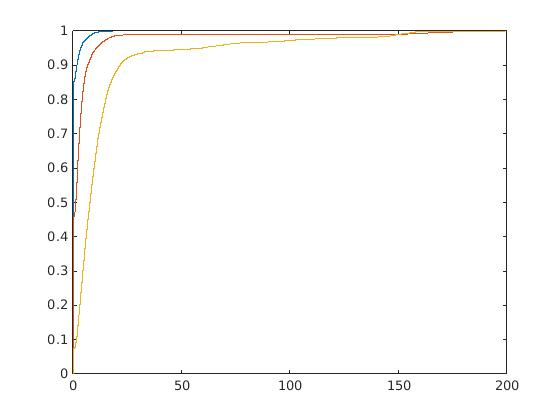
\includegraphics[height = 3cm]{figures/horse910_200.jpg}
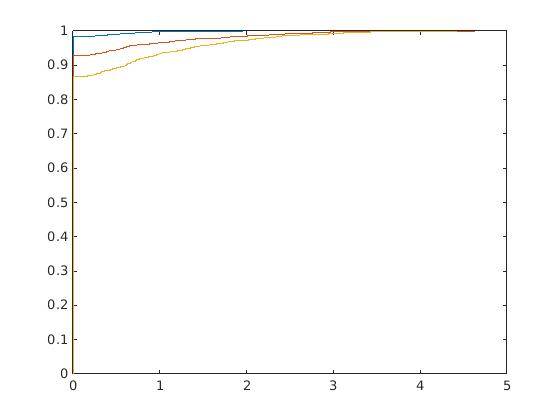
\includegraphics[height = 3cm]{figures/wolf2_200.jpg}
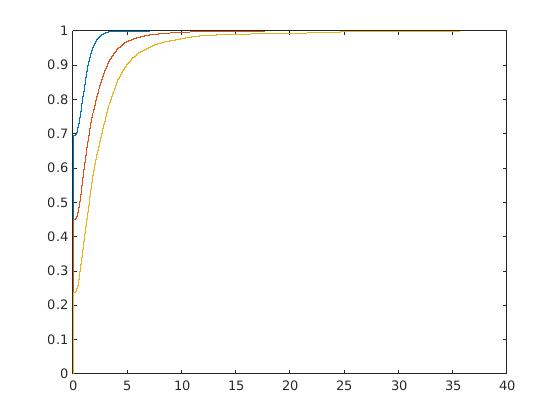
\includegraphics[height = 3cm]{figures/dog1105_200.jpg}
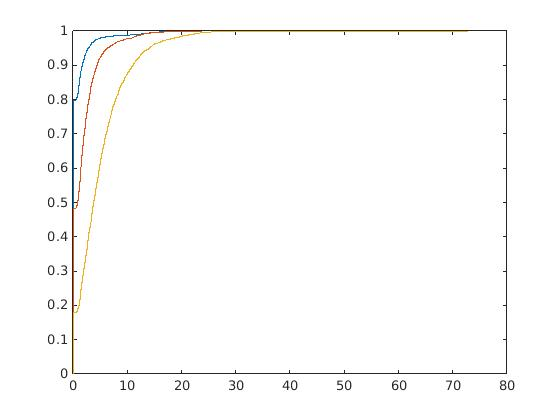
\includegraphics[height = 3cm]{figures/cat5_100.jpg}
\includegraphics[height = 3cm]{figures/human1407_200.jpg}  
\includegraphics[height = 3cm]{figures/centaur704_200.jpg} 
\caption[Improvements measured with functional maps]{\label{fig:improvements} The blue curve represents the correspondence induced by the ground-truth functional map. The yellow one
		represents the correspondence induced by the optimal functional map without the topological vectors and the red one 
		represents the correspondence induced by the optimal functional map with the vectors. 
		The categories are, from left to right and top to bottom: horse, wolf, dog, cat, human and centaur.}
\end{center}
\end{figure*}



\begin{figure*}[t!] 
\begin{center} 
\includegraphics[height = 2cm]{figures/imprhorse910}
\includegraphics[height = 2cm]{figures/imprwolf2}  
\includegraphics[height = 2cm]{figures/imprdog1105}  
\includegraphics[height = 2cm]{figures/imprcat7}  
\includegraphics[height = 2cm]{figures/imprhuman1407}
\includegraphics[height = 2cm]{figures/imprcentaur704}  

\caption[Improvements measured directly on shapes]{\label{fig:improvementsonshape} Yellow parts are the ones which are the most improved with the topological vectors. 
        Dark blue means no improvement. For every shape, it is clear: firstly that there is a positive improvement almost everywhere
	      and secondly that the best improvements are obtained on the flat parts of the shapes.}
\end{center}
\end{figure*}


\section{Conclusion}

In this chapter, we introduced the {\em Sliced Wasserstein kernel} and the {\em topological vectors},
which are two possible kernels for persistence diagrams that are provably {\em stable} with respect to $\distw{1}$,
the Sliced Wasserstein kernel being even equivalent to it for persistence diagrams with bounded cardinalities.
%to the first diagram distance between persistence diagrams. 
We provided algorithms for computation,
and we showed on several datasets substantial improvements in accuracy and training times 
(when tuning parameters is done with grid search) over competing kernels. 
%A particularly appealing property of that kernel is that it is infinitely divisible, 
%substantially facilitating the tuning of parameters through cross validation.

\paragraph*{Metric properties of embeddings.}
Even though the Sliced Wasserstein kernel is provably equivalent to $\distw{1}$, the lower bound
depends on the number of diagram points, and converges to zero when the number of points increases.
Our intuition is that this is the case for any mapping of persistence diagrams, i.e. either the upper or the lower bound
depends on the number of points, and either converges to $+\infty$ (for the upper bound) or $0$ (for the lower bound) when the number
of points increases. Hence, we believe that a study about quantifying the metric distortion of a general mapping of persistence diagrams
into a (possibly infinite dimensional) Hilbert space is possible and worth considering. 


%\bibliographystyle{plain}
%\bibliography{biblio}
